%For DESY PC
\documentclass[xcolor=dvipsnames,compress,DESYcyan,9pt,unknownkeysallowed]{beamer}

\newcommand{\logopath}{../Logos}


\usepackage{blindtext}
% \usepackage[utf8,latin1]{inputenc}
\usepackage[T1]{fontenc}
\usepackage[english]{babel}
\usepackage{amsmath, amscd} %amscd for commutative diagrams
\usepackage{mathtools}
\usepackage{amssymb}
\usepackage{array}
\usepackage{blkarray}
\usepackage{color}
\usepackage{enumerate}
\usepackage{fancybox}
\usepackage{float}
\usepackage[hang]{footmisc}
\usepackage{graphicx}
\usepackage{listings}
\usepackage{lmodern}
\usepackage{multirow}
\usepackage{pifont}
\usepackage{rotating}
\usepackage[small, sl, SL,sf, SF, bf, hang, raggedright]{subfigure}
\usepackage{tabularx}
\usepackage{tcolorbox}
\usepackage{textpos}
\usepackage{textcomp}
\usepackage{tikz}
\usepackage{upgreek}
\usepackage{appendixnumberbeamer}
\usepackage{courier} % For programming style font

\definecolor{DESYcyan}{RGB}{0,166,235}
\definecolor{DESYorange}{RGB}{242,142,0}
\definecolor{DESYgray}{RGB}{119,119,119}
\definecolor{bjetpurple}{RGB}{117,112,179}

\usepackage[font=footnotesize,labelfont={color=DESYorange,footnotesize}]{caption}

\usepackage{xcolor}
\definecolor{light-gray}{gray}{0.8}
\usepackage{relsize}
\renewcommand*{\UrlFont}{\ttfamily\smaller\relax}
\usepackage{hyperref}
\hypersetup{
	colorlinks=true,
	linkcolor=black,
	filecolor=black,
	urlcolor=black,%light-gray,
	breaklinks=true
}



\usepackage[compat=1.1.0]{tikz-feynman}
\usepackage{contour}

\usetikzlibrary{arrows,shapes,positioning}
\usetikzlibrary{decorations.markings}
\usetikzlibrary{decorations.pathmorphing}
\usetikzlibrary{decorations.pathreplacing}
\usetikzlibrary{patterns}
\usetikzlibrary{plotmarks}
\usetikzlibrary{shadows}

\tcbuselibrary{skins}

% \tikzstyle arrowstyle=[scale=1.5]
% \tikzstyle directed=[postaction={decorate,decoration={markings,
%    mark=at position .55 with {\arrow[arrowstyle]{stealth}}}}]
% \tikzstyle reverse directed=[postaction={decorate,decoration={markings,
%    mark=at position .55 with {\arrowreversed[arrowstyle]{stealth};}}}]
% \tikzset{
%    boson/.style={decorate, decoration={snake}, draw=black},
%    fermion/.style={draw=black, postaction={decorate},
%        decoration={markings,mark=at position .6 with {\arrow[arrowstyle]{stealth}}}},
%    fbar/.style={draw=black, postaction={decorate},
%        decoration={markings,mark=at position .6 with {\arrowreversed[arrowstyle]{stealth}}}},
%    gluon/.style={decorate, draw=black,
%        decoration={coil,amplitude=4pt, segment length=5pt}},
% }

\newcommand*\at{{\fontfamily{ptm}\selectfont @}}


%%%%%%%%%%%%%%%%%%%%%%%%%%%%%%%%%%%%%%%%%%%%%%%%%%%%%%%%%%%%%%%%%%%%%%%%%%%%%%%
% Code:

\usepackage{ulem} %for underline, crossing our, etc...

\lstset{
%backgroundcolor=\color{lbcolor},
    tabsize=2,
%   rulecolor=,
    language=[GNU]C++,
    % linewidth=0.9\textwidth,
    xleftmargin=.1\textwidth,
        basicstyle=\scriptsize,
        upquote=true,
        aboveskip={1.5\baselineskip},
        columns=fixed,
        showstringspaces=false,
        extendedchars=false,
        breaklines=true,
        prebreak = \raisebox{0ex}[0ex][0ex]{\ensuremath{\hookleftarrow}},
        frame=single,
        % numbers=left,
        showtabs=false,
        showspaces=false,
        showstringspaces=false,
        identifierstyle=\ttfamily,
        keywordstyle=\color[rgb]{0,0,1},
        commentstyle=\color[rgb]{0.026,0.112,0.095},
        stringstyle=\color[rgb]{0.627,0.126,0.941},
        numberstyle=\color[rgb]{0.205, 0.142, 0.73},
%        \lstdefinestyle{C++}{language=C++,style=numbers}’.
    texcl=true,
}

% \usepackage{filecontent}

\newsavebox\mybox

%%%%%%%%%%%%%%%%%%%%%%%%%%%%%%%%%%%%%%%%%%%%%%%%%%%%%%%%%%%%%%%%%%%%%%%%%%%%%%%


\setlength\footnotemargin{10pt}

\let\beginoldtabular=\tabular
\let\endoldtabular\endtabular
\renewenvironment{tabular}
{
	\def\arraystretch{1.5}
	\beginoldtabular
}
{
	\endoldtabular
}

\newcolumntype{C}{>{\centering\arraybackslash}X}
\let\beginoldtabularx=\tabularx
\let\endoldtabularx\endtabularx
\renewenvironment{tabularx}
{
	\def\arraystretch{1.5}
	\beginoldtabularx
}
{
	\endoldtabularx
}


\usepackage{beamerthemesplit}



% \usetheme{CambridgeUS}
\usefonttheme[onlymath]{serif}
\usecolortheme[named=DESYcyan]{structure}
\useoutertheme{infolines}
% \useoutertheme{default}


\setbeamercolor{palette primary}{bg=white}
\setbeamercolor{section in head/foot}{bg=DESYcyan, fg=white}
\setbeamercolor{frametitle}{fg=DESYcyan,bg=white}
\setbeamerfont{frametitle}{series=\bfseries, size=\LARGE}
\setbeamercolor{framesubtitle}{fg=DESYorange,bg=white}
\setbeamerfont{framesubtitle}{series=\bfseries}
\addtobeamertemplate{headline}{\hypersetup{linkcolor=white}\vspace*{0.7em}}{\vspace*{-0.2em}}
% \setbeamertemplate{headline}{\leavevmode \hypersetup{linkcolor=white} }

\setbeamercolor{item}{fg=DESYorange}
\setbeamercolor{subitem}{fg=DESYcyan}
\setbeamercolor{subsubitem}{fg=DESYgray}

\setbeamertemplate{navigation symbols}{}
\setbeamertemplate{footline}{}
\setbeamertemplate{bibliography item}[text]


% \addtobeamertemplate{footline}{}{
% \begin{textblock*}{1cm}[1,1](12.6cm,-0.1cm)  %(5cm,5cm)
% 
\includegraphics[height=1cm]{\logopath/DESY-logo.jpg}
% \end{textblock*}
% }

\addtobeamertemplate{footline}{}{
\begin{textblock*}{0.9\textwidth}[-0.1,1](-0.5cm, -0.3cm)  %(5cm,5cm)
\textbf{\textcolor{DESYcyan}{DESY}\textcolor{DESYorange}{.}} ~$|$ \insertshorttitle ~$|$ \insertshortauthor ~$|$ \insertdate ~$|$ \hfill Page \insertframenumber/\inserttotalframenumber
\end{textblock*}
\begin{textblock*}{0.9\textwidth}[-0.1,1](5cm,5cm)
\end{textblock*}
}

 \newenvironment{mydesybox}[2]
 {
 	\begin{minipage}{#1}
	\begin{tcolorbox}[beamer,enhanced, colback=DESYcyan!2!white, colframe=DESYcyan, boxrule=0.5mm, title=#2]
}
{
	\end{tcolorbox}
	\end{minipage}
}

\newenvironment{mydesyinlinebox}[2]
{\begin{tcolorbox}[beamer,enhanced, colback=DESYcyan!2!white, colframe=DESYcyan, boxrule=0.5mm, title=#2]  }
{\end{tcolorbox}}

\tcbset{colframe=DESYcyan, colback=DESYcyan!2!white, colupper=black, fonttitle=\bfseries,nobeforeafter,center title}


\setbeamercolor{title}{fg=DESYcyan}
\setbeamerfont{title}{series=\bfseries, size=}
\setbeamercolor{subtitle}{fg=DESYorange}


\setbeamertemplate{title page}
{
  \vbox{}
\vfill
  \begin{flushleft}
    \begin{beamercolorbox}[sep=8pt, size=\Huge]{title}%,center]{title}
      \usebeamerfont{title}%
			{\Huge\inserttitle}\par%
      \ifx\insertsubtitle\@empty%
      \else%
        \vskip0.25em%
        {\usebeamerfont{subtitle}\usebeamercolor[fg]{subtitle}\insertsubtitle\par}%
      \fi%
    \end{beamercolorbox}%
    \vskip1em\par
    \begin{beamercolorbox}[sep=8pt]{author}%,center
      \usebeamerfont{author}\insertauthor
    \end{beamercolorbox} \vspace{-0.7em}
    \begin{beamercolorbox}[sep=8pt]{institute} %,center
      \usebeamerfont{institute}\normalbaselines\insertinstitute
    \end{beamercolorbox} \vspace{-0.5em}
    \begin{beamercolorbox}[sep=8pt]{date} %,center
      \usebeamerfont{date}\insertdate
    \end{beamercolorbox}
    \vskip 1em
    \vfill

	% \hfill
	\hspace{8pt}
	\begin{minipage}{0.35\textwidth}
		\vspace{0.7cm} \vspace{1em}
		
\includegraphics[height=0.7cm]{\logopath/DESY-logo.jpg}
		% \hfill
		% \hfill
		\hspace{0.2em}
    
\includegraphics[height=0.7cm]{\logopath/2017_H_Logo_CMYK_untereinander_EN.jpg}
    \hfill
	\end{minipage}
	\hfill
	\begin{minipage}{0.6\textwidth}  \raggedleft
    \hfill
		
\includegraphics[height=0.7cm]{\logopath/LCC-logo.jpg}
		\hspace{0.2cm}
		
\includegraphics[height=0.7cm]{\logopath/ILC-logo.jpg}
		\hspace{0.2cm}
		
\includegraphics[height=0.7cm]{\logopath/ildlogo_Zh-mumuh_sharper_whiteonblue.png}
		\vspace{1em}\\
    \hfill
    
\includegraphics[height=0.7cm]{\logopath/university-of-cambridge-logo.png}
	\end{minipage}
\end{flushleft}
  %\vfill
}



\newcommand{\myitem}{\item[\ding{228}]}

\newcommand{\makemytitlepage}{\frame[plain]{\titlepage}}

\newcommand{\BackUp}{\appendix\frame{\begin{center}\begin{Huge}Backup Slides\end{Huge}\end{center}}}





%%%%%%%%%%%%%%%%%%%%%%%%%%%%%%%%%%%%%%%%%%%%%%%%%%%%%%%%%%%%%%%%%%%%%%%%%%%%%%%
% Shadowed Images

\usetikzlibrary{shadows,calc}

% code adapted from https://tex.stackexchange.com/a/11483/3954

% some parameters for customization
\def\shadowshift{3pt,-3pt}
\def\shadowradius{6pt}

\colorlet{innercolor}{black!60}
\colorlet{outercolor}{gray!05}

% this draws a shadow under a rectangle node
\newcommand\drawshadow[1]{
    \begin{pgfonlayer}{shadow}
        \shade[outercolor,inner color=innercolor,outer color=outercolor] ($(#1.south west)+(\shadowshift)+(\shadowradius/2,\shadowradius/2)$) circle (\shadowradius);
        \shade[outercolor,inner color=innercolor,outer color=outercolor] ($(#1.north west)+(\shadowshift)+(\shadowradius/2,-\shadowradius/2)$) circle (\shadowradius);
        \shade[outercolor,inner color=innercolor,outer color=outercolor] ($(#1.south east)+(\shadowshift)+(-\shadowradius/2,\shadowradius/2)$) circle (\shadowradius);
        \shade[outercolor,inner color=innercolor,outer color=outercolor] ($(#1.north east)+(\shadowshift)+(-\shadowradius/2,-\shadowradius/2)$) circle (\shadowradius);
        \shade[top color=innercolor,bottom color=outercolor] ($(#1.south west)+(\shadowshift)+(\shadowradius/2,-\shadowradius/2)$) rectangle ($(#1.south east)+(\shadowshift)+(-\shadowradius/2,\shadowradius/2)$);
        \shade[left color=innercolor,right color=outercolor] ($(#1.south east)+(\shadowshift)+(-\shadowradius/2,\shadowradius/2)$) rectangle ($(#1.north east)+(\shadowshift)+(\shadowradius/2,-\shadowradius/2)$);
        \shade[bottom color=innercolor,top color=outercolor] ($(#1.north west)+(\shadowshift)+(\shadowradius/2,-\shadowradius/2)$) rectangle ($(#1.north east)+(\shadowshift)+(-\shadowradius/2,\shadowradius/2)$);
        \shade[outercolor,right color=innercolor,left color=outercolor] ($(#1.south west)+(\shadowshift)+(-\shadowradius/2,\shadowradius/2)$) rectangle ($(#1.north west)+(\shadowshift)+(\shadowradius/2,-\shadowradius/2)$);
        \filldraw ($(#1.south west)+(\shadowshift)+(\shadowradius/2,\shadowradius/2)$) rectangle ($(#1.north east)+(\shadowshift)-(\shadowradius/2,\shadowradius/2)$);
    \end{pgfonlayer}
}

% create a shadow layer, so that we don't need to worry about overdrawing other things
\pgfdeclarelayer{shadow}
\pgfsetlayers{shadow,main}


\newcommand\shadowimage[2][]{%
\begin{tikzpicture}
\node[anchor=south west,inner sep=0] (image) at (0,0) {\includegraphics[#1]{#2}};
\drawshadow{image}
\end{tikzpicture}}
%%%%%%%%%%%%%%%%%%%%%%%%%%%%%%%%%%%%%%%%%%%%%%%%%%%%%%%%%%%%%%%%%%%%%%%%%%%%%%%
% New symbols


\newcommand{\Lagr}{\mathcal{L}} % Lagrangian-L
\newcommand{\oper}{\mathcal{O}} % Operator symbol

%%%%%%%%%%%%%%%%%%%%%%%%%%%%%%%%%%%%%%%%%%%%%%%%%%%%%%%%%%%%%%%%%%%%%%%%%%%%%%%
% DESY text colors

\newcommand\OrangeBF[1]{\textcolor{DESYorange}{\textbf{#1}}}
\newcommand\CyanBF[1]{\textcolor{DESYcyan}{\textbf{#1}}}

%%%%%%%%%%%%%%%%%%%%%%%%%%%%%%%%%%%%%%%%%%%%%%%%%%%%%%%%%%%%%%%%%%%%%%%%%%%%%%%
% Convenient way to set border around input

\newcommand\scaledinput[2][]{
  \scalebox{#1}{\input{#2}}
}

%%%%%%%%%%%%%%%%%%%%%%%%%%%%%%%%%%%%%%%%%%%%%%%%%%%%%%%%%%%%%%%%%%%%%%%%%%%%%%%
% Rotated text

\usepackage{rotating}

%%%%%%%%%%%%%%%%%%%%%%%%%%%%%%%%%%%%%%%%%%%%%%%%%%%%%%%%%%%%%%%%%%%%%%%%%%%%%%%
% Particles
\newcommand{\eP}{e^{+}}
\newcommand{\eM}{e^{-}}
\newcommand{\lP}{l^{+}}
\newcommand{\lM}{l^{-}}

\newcommand{\fbar}{\bar{f}}
\newcommand{\mubar}{\bar{\mu}}

\newcommand{\eL}{\eM_{L}}
\newcommand{\eR}{\eM_{R}}
\newcommand{\pL}{\eP_{L}}
\newcommand{\pR}{\eP_{R}}

\newcommand{\nue}{\nu_e}
\newcommand{\numu}{\nu_{\mu}}
\newcommand{\nutau}{\nu_{\tau}}
\newcommand{\nul}{\nu_l}

\newcommand{\nubar}{\bar{\nu}}
\newcommand{\nuebar}{\bar{\nue}}
\newcommand{\nulbar}{\bar{\nul}}

\newcommand{\qbar}{\bar{q}}
\newcommand{\qu}{q_{u}}
\newcommand{\qd}{q_{d}}
\newcommand{\qubar}{\bar{q}_{u}}
\newcommand{\qdbar}{\bar{q}_{d}}

\newcommand{\tbar}{\bar{t}}

\newcommand{\vis}{\text{vis}}
\newcommand{\inv}{\text{inv}}

\newcommand{\WP}{W^{+}}
\newcommand{\WM}{W^{-}}
%%%%%%%%%%%%%%%%%%%%%%%%%%%%%%%%%%%%%%%%%%%%%%%%%%%%%%%%%%%%%%%%%%%%%%%%%%%%%%%
% Checkmark

\def\checkmark{\tikz\fill[scale=0.4](0,.35) -- (.25,0) -- (1,.7) -- (.25,.15) -- cycle;}
%%%%%%%%%%%%%%%%%%%%%%%%%%%%%%%%%%%%%%%%%%%%%%%%%%%%%%%%%%%%%%%%%%%%%%%%%%%%%%%
% Allow Latex over included graphic
\usepackage[percent]{overpic}

%%%%%%%%%%%%%%%%%%%%%%%%%%%%%%%%%%%%%%%%%%%%%%%%%%%%%%%%%%%%%%%%%%%%%%%%%%%%%%%
% Package for additional symbols like cross-x
\usepackage{pifont}
\newcommand{\xmark}{\ding{55}}%

%%%%%%%%%%%%%%%%%%%%%%%%%%%%%%%%%%%%%%%%%%%%%%%%%%%%%%%%%%%%%%%%%%%%%%%%%%%%%%%
% Allow line-breaks in tabular cell
\usepackage{makecell}

%%%%%%%%%%%%%%%%%%%%%%%%%%%%%%%%%%%%%%%%%%%%%%%%%%%%%%%%%%%%%%%%%%%%%%%%%%%%%%%


\title[Angular efficiencies of semileptonic W pair decay at the ILC]{Angular efficiencies of semileptonic W pair decay at the ILC}
\subtitle{FLC group presentation}
\author[Matthew Koster]{Matthew Koster\inst{1,2} \\Supervisor: Jakob Beyer \inst{1,3}}% \inst{1,2} \and author2 \inst{2}}
\institute[shortinst]{\inst{1} DESY Hamburg \and %
                      \inst{2} University of Cambridge \and %
                      \inst{3} Universit\"at Hamburg}
\date{September 2, 2019}

\newcommand{\imagepath}{../Plots}
\newcommand{\feynmanpath}{../FeynmanDiagrams}

\begin{document}

%WARNING: Needs to be compiled using lualatex (might work w/o, look at Feynman diagrams)

% ----------------------------------------------------------------------------
% ----------------------------------------------------------------------------

\makemytitlepage
% TODO Something about GitHub & Confluence pages and IDR notes

% ----------------------------------------------------------------------------
% ----------------------------------------------------------------------------

\begin{frame}\frametitle{W pair production \OrangeBF{and chiral structures}}

    \begin{minipage}{0.49\textwidth}
        \begin{itemize}
            \setlength\itemsep{2em}
            \item Chiral structure of weak interaction
            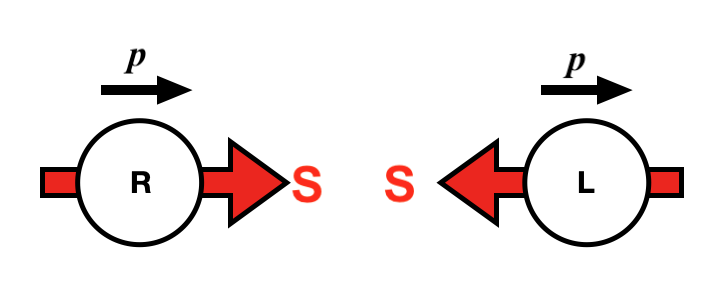
\includegraphics[width=0.8\textwidth, center]{\imagepath/Chirality.png}
            \item initial state ${e}_{L}^{-} {e}_{R}^{+}$
        \end{itemize}
    \end{minipage}
    \begin{minipage}{0.49\textwidth}
        \centering
        \begin{tikzpicture}
  \begin{feynman}[scale=1] % using the vertex in brackets () allows fixing of vertex
    \vertex (a) at (-0.75, 0) ;
    \vertex (c) at (0.75, 0) ;
    \vertex (b) at (2.25,-1) {$W^-$};
    \vertex (d) at (2.25, 1) {$W^+$};
    \vertex (i1) at (-2.25,-1) {$e^-$};
    \vertex (i2) at (-2.25, 1) {$e^+$};
    \diagram* {
      (i1) -- [fermion] (a) ,
      (i2) -- [anti fermion] (a) ,
      (a) -- [photon, edge label=$Z/\gamma$] (c),
      (b) -- [photon] (c),
      (d) -- [photon] (c),
    };
  \end{feynman}
\end{tikzpicture}

        \bigskip
        \centering
        \begin{tikzpicture}
  \begin{feynman}[scale=1] % using the vertex in brackets () allows fixing of vertex
    \vertex (a) at (0, 0.5) ;
    \vertex (c) at (0, -0.5) ;
    \vertex (b) at ( 2,-1) {$W^-$};
    \vertex (d) at ( 2, 1) {$W^+$};
    \vertex (i1) at (-2,-1) {$e_L^-$};
    \vertex (i2) at (-2, 1) {$e_R^+$};
    \diagram* {
      (i1) -- [fermion] (c) -- [fermion, edge label=$\nu_e$] (a),
      (i2) -- [anti fermion] (a),
      (b) -- [photon] (c),
      (d) -- [photon] (a),

    };
  \end{feynman}
\end{tikzpicture}

    \end{minipage}

\end{frame}

% ----------------------------------------------------------------------------

\begin{frame}\frametitle{Neutrino and ISR Corrections \OrangeBF{The hard collision}}

    \begin{minipage}{0.49\textwidth}
        \CyanBF{The final state}\\
        \begin{itemize}\setlength\itemsep{1em}
            \item \CyanBF{Visible 4-momenta} ${p}^{\mu} = ( E, {p}_{x}, {p}_{y}, {p}_{z} )$
            \item \CyanBF{Neutrino 4-momenta} ${p}_{\nu}^{\mu} = (  {E}_{\nu}, {p}_{x, \nu}, {p}_{y, \nu}, {p}_{z, \nu} )$
            \item \CyanBF{ISR Photon 4-momenta} ${p}_{\gamma}^{\mu} = ( {E}_{\gamma}, 0, 0, {p}_{\gamma} )$
        \end{itemize}
    \end{minipage}\hfill
    \begin{minipage}{0.49\textwidth}
        \resizebox{\linewidth}{!}{%
        \centering
        \begin{tikzpicture}
  \begin{feynman}[scale=1] % using the vertex in brackets () allows fixing of vertex
    \vertex (m) at (-1, 0);
    \vertex (n) at (0.5, 0);

    \vertex (r) at (-1.7,-0.5);
    \vertex (s) at (-1.7, 0.5);

    \vertex (a) at (-1.5,-1);s
    \vertex (b) at ( 1.75,-1) ;
    \vertex (c) at (-1.5, 1);
    \vertex (d) at ( 1.75, 1) ;

    \vertex (u) at ( 3.5,-1.5) {$l^-$};
    \vertex (v) at ( 3.5,-0.5) {$\bar{\nu}_l$};

    \vertex (q1) at ( 3.5, 1.5) {$q$};
    \vertex (q2) at ( 3.5, 0.5) {$\bar{q'}$};

    \vertex (i1) at (-3,-1) {$e^-$};
    \vertex (i2) at (-3, 1) {$e^+$};

    \vertex (p1) at (0,-1.5) {$\gamma$};
    \vertex (p2) at (0, 1.5) {$\gamma$};

    \diagram* {
      (i1) -- [fermion] (r) --[fermion] (m) ,
      (i2) -- [anti fermion] (s) -- [anti fermion] (m) ,
      (m) -- [photon, edge label=$Z/\gamma$] (n),
      (b) -- [photon, edge label=$W^-$, swap] (n),
      (d) -- [photon, edge label=$W^+$] (n),
      (b) -- [fermion] (u),
      (b) -- [anti fermion] (v),
      (d) -- [fermion] (q1),
      (d) -- [anti fermion] (q2),
      (r) -- [photon] (p1),
      (s) -- [photon] (p2),
    };
  \end{feynman}
\end{tikzpicture}

        }
        \\
        \centering
        \begin{tikzpicture}
  \begin{feynman}[scale=1] % using the vertex in brackets () allows fixing of vertex
    \vertex (n) at (0, 0.75) ;
    \vertex (m) at (0, -0.75) ;

    \vertex (r) at (-1.2,-1);
    \vertex (s) at (-1.2, 1);

    \vertex (a) at (-1,-1) ;
    \vertex (b) at ( 1.25,-1) ;
    \vertex (c) at (-1, 1);
    \vertex (d) at ( 1.25, 1) ;

    \vertex (u) at ( 3,-1.5) {$l^-$};
    \vertex (v) at ( 3,-0.5) {$\bar{\nu}_l$};

    \vertex (q1) at ( 3, 1.5) {$q$};
    \vertex (q2) at ( 3, 0.5) {$\bar{q'}$};

    \vertex (i1) at (-2.5,-1) {$e_L^-$};
    \vertex (i2) at (-2.5, 1) {$e_R^+$};

    \vertex (p1) at (0,-1.5) {$\gamma$};
    \vertex (p2) at (0, 1.5) {$\gamma$};


    \diagram* {
      (i1) -- [fermion] (r) --[fermion] (m) -- [fermion, edge label=$\nu_e$] (n),
      (i2) -- [anti fermion] (s) -- [anti fermion] (n),
      (b) -- [photon, edge label=$W^-$, swap] (m),
      (d) -- [photon, edge label=$W^+$] (n),
      (b) -- [fermion] (u),
      (b) -- [anti fermion] (v),
      (d) -- [fermion] (q1),
      (d) -- [anti fermion] (q2),
      (r) -- [photon] (p1),
      (s) -- [photon] (p2),

    };
  \end{feynman}
\end{tikzpicture}

    \end{minipage}

\end{frame}
% ----------------------------------------------------------------------------

\begin{frame}\frametitle{Neutrino and ISR Corrections \OrangeBF{ISR energy}}

    \begin{minipage}{0.49\textwidth}
        \centering
        Energy conservation \\
        + \\
        momentum conservation\\
        = \\
        \CyanBF{ISR energy equation}
        \begin{equation*}
            {E}_{\gamma} = \frac{ {( \sqrt{s} - E )}^2 - {p}^{2} }{2 \sqrt{s} -2 E  \mp 2{p}_{z}}
        \end{equation*}
        \\ \hfill \\
        $ \sqrt{s} = 500 $ GeV
    \end{minipage}\hfill
    \begin{minipage}{0.49\textwidth}
        \resizebox{\linewidth}{!}{%
        \centering
        \begin{tikzpicture}
  \begin{feynman}[scale=1] % using the vertex in brackets () allows fixing of vertex
    \vertex (m) at (-1, 0);
    \vertex (n) at (0.5, 0);

    \vertex (r) at (-1.7,-0.5);
    \vertex (s) at (-1.7, 0.5);

    \vertex (a) at (-1.5,-1);s
    \vertex (b) at ( 1.75,-1) ;
    \vertex (c) at (-1.5, 1);
    \vertex (d) at ( 1.75, 1) ;

    \vertex (u) at ( 3.5,-1.5) {$l^-$};
    \vertex (v) at ( 3.5,-0.5) {$\bar{\nu}_l$};

    \vertex (q1) at ( 3.5, 1.5) {$q$};
    \vertex (q2) at ( 3.5, 0.5) {$\bar{q'}$};

    \vertex (i1) at (-3,-1) {$e^-$};
    \vertex (i2) at (-3, 1) {$e^+$};

    \vertex (p1) at (0,-1.5) {$\gamma$};
    \vertex (p2) at (0, 1.5) {$\gamma$};

    \diagram* {
      (i1) -- [fermion] (r) --[fermion] (m) ,
      (i2) -- [anti fermion] (s) -- [anti fermion] (m) ,
      (m) -- [photon, edge label=$Z/\gamma$] (n),
      (b) -- [photon, edge label=$W^-$, swap] (n),
      (d) -- [photon, edge label=$W^+$] (n),
      (b) -- [fermion] (u),
      (b) -- [anti fermion] (v),
      (d) -- [fermion] (q1),
      (d) -- [anti fermion] (q2),
      (r) -- [photon] (p1),
      (s) -- [photon] (p2),
    };
  \end{feynman}
\end{tikzpicture}

        }
        \\
        \centering
        \begin{tikzpicture}
  \begin{feynman}[scale=1] % using the vertex in brackets () allows fixing of vertex
    \vertex (n) at (0, 0.75) ;
    \vertex (m) at (0, -0.75) ;

    \vertex (r) at (-1.2,-1);
    \vertex (s) at (-1.2, 1);

    \vertex (a) at (-1,-1) ;
    \vertex (b) at ( 1.25,-1) ;
    \vertex (c) at (-1, 1);
    \vertex (d) at ( 1.25, 1) ;

    \vertex (u) at ( 3,-1.5) {$l^-$};
    \vertex (v) at ( 3,-0.5) {$\bar{\nu}_l$};

    \vertex (q1) at ( 3, 1.5) {$q$};
    \vertex (q2) at ( 3, 0.5) {$\bar{q'}$};

    \vertex (i1) at (-2.5,-1) {$e_L^-$};
    \vertex (i2) at (-2.5, 1) {$e_R^+$};

    \vertex (p1) at (0,-1.5) {$\gamma$};
    \vertex (p2) at (0, 1.5) {$\gamma$};


    \diagram* {
      (i1) -- [fermion] (r) --[fermion] (m) -- [fermion, edge label=$\nu_e$] (n),
      (i2) -- [anti fermion] (s) -- [anti fermion] (n),
      (b) -- [photon, edge label=$W^-$, swap] (m),
      (d) -- [photon, edge label=$W^+$] (n),
      (b) -- [fermion] (u),
      (b) -- [anti fermion] (v),
      (d) -- [fermion] (q1),
      (d) -- [anti fermion] (q2),
      (r) -- [photon] (p1),
      (s) -- [photon] (p2),

    };
  \end{feynman}
\end{tikzpicture}

    \end{minipage}

\end{frame}

% ----------------------------------------------------------------------------

\begin{frame}\frametitle{Neutrino and ISR Corrections \OrangeBF{${E}_{\gamma} = 0$ solution}}

    Only considering muon signal
    \centering
    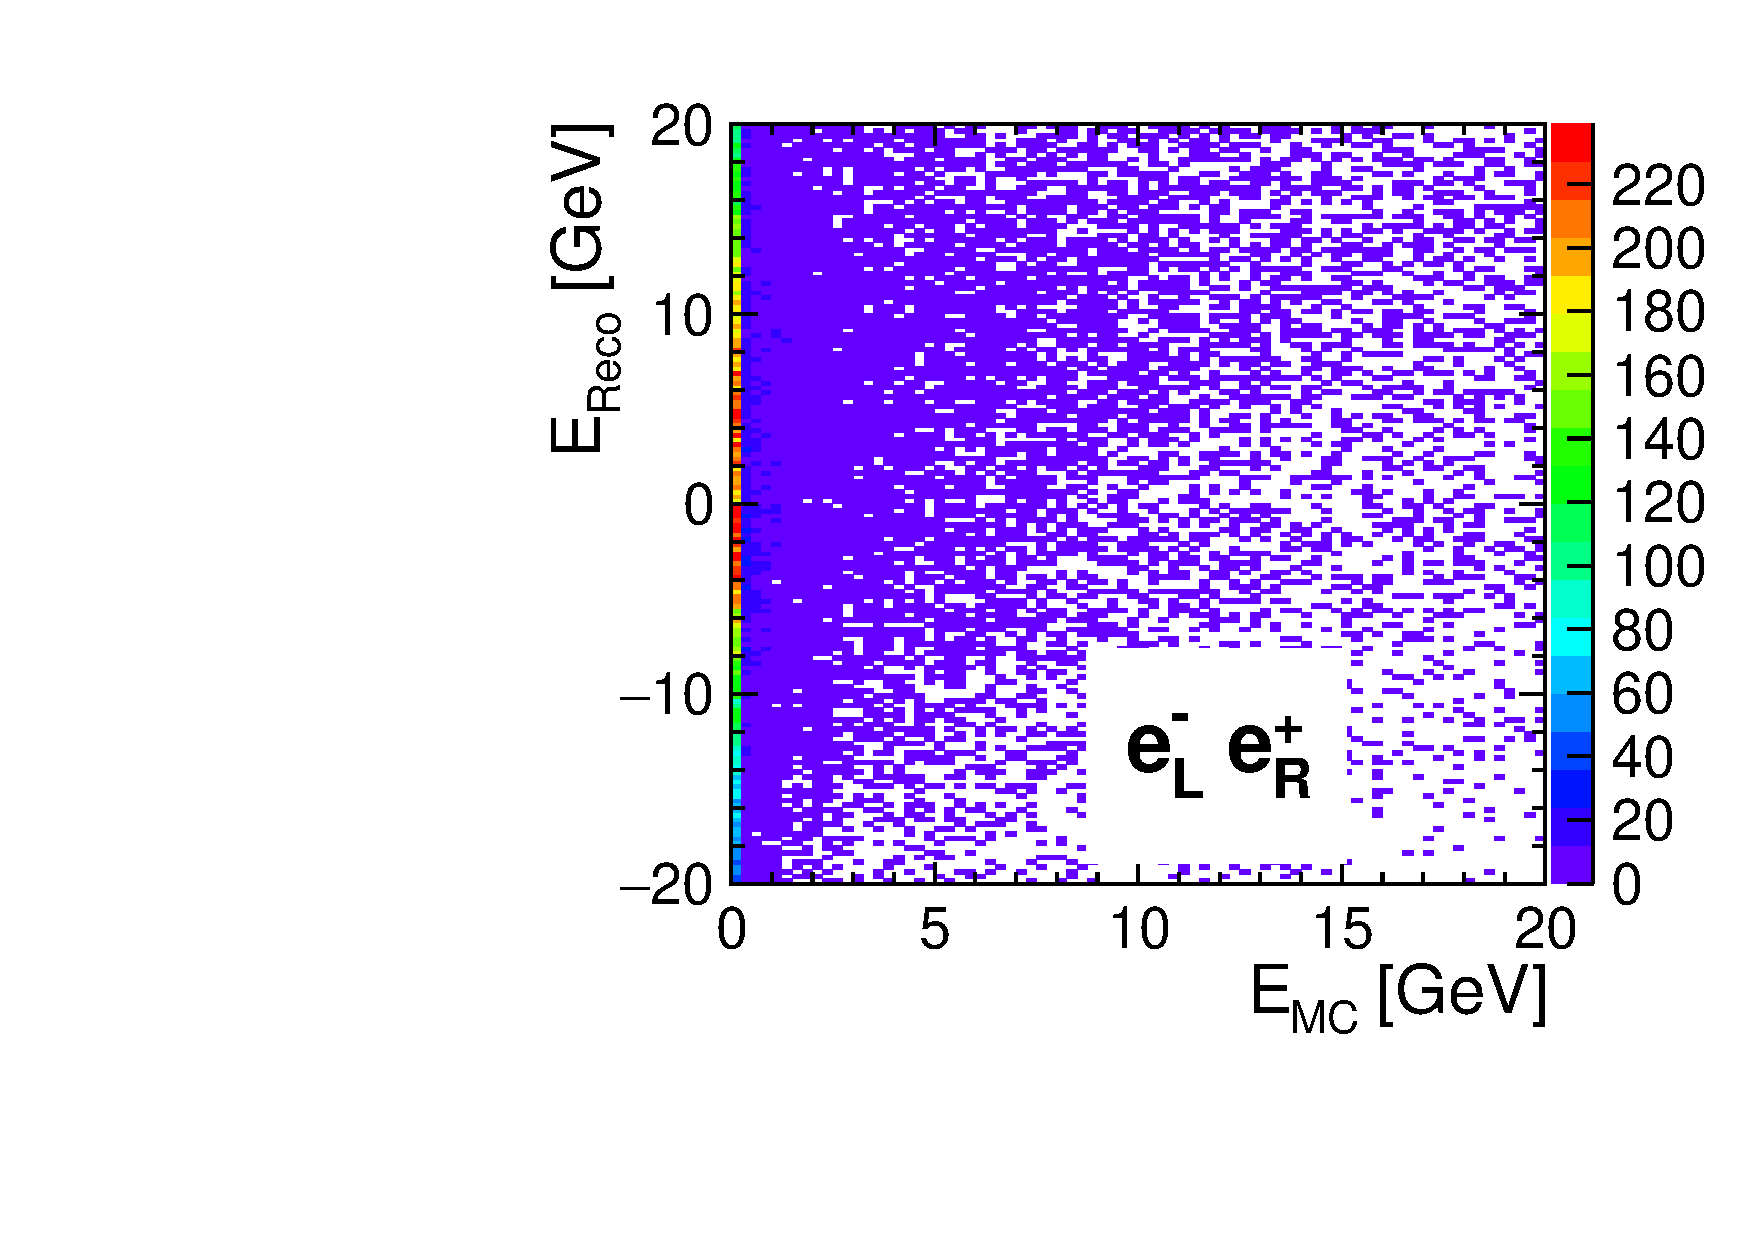
\includegraphics[width=0.7\textwidth, top]{\imagepath/PhotonEnergy_2D.pdf}

\end{frame}

% ----------------------------------------------------------------------------

\begin{frame}\frametitle{Neutrino and ISR Corrections \OrangeBF{Reconstruction evaluation}}

    Only considering muon signal
    \centering
    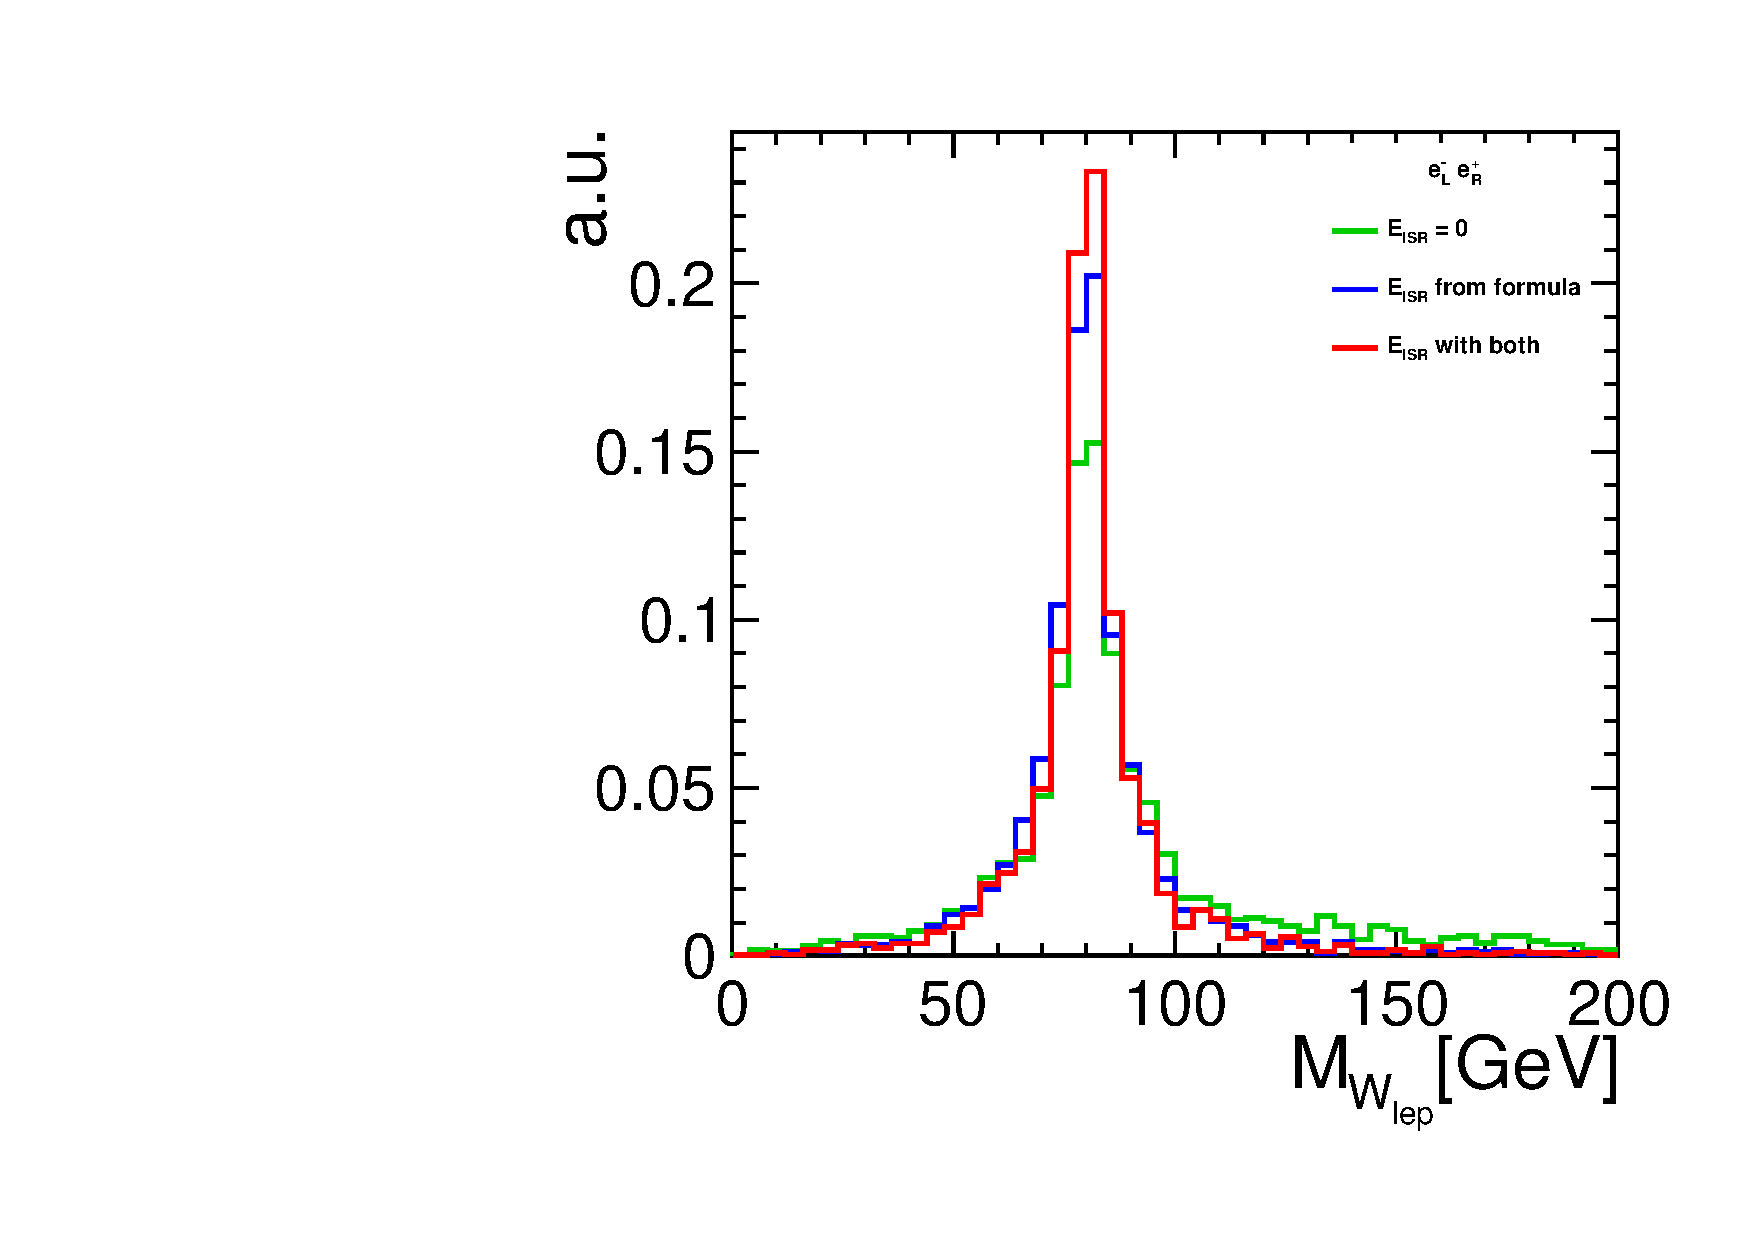
\includegraphics[width=0.7\textwidth, top]{\imagepath/Mass3.pdf}

\end{frame}

% ----------------------------------------------------------------------------

\begin{frame}\frametitle{Angle Extractions \OrangeBF{Angle definitions}}

    \begin{minipage}{0.49\textwidth}
        Angles ${\theta}_{W^{-}}, {\theta}_{l}^{*}, {\phi}_{l}^{*}$\\
        \centering
        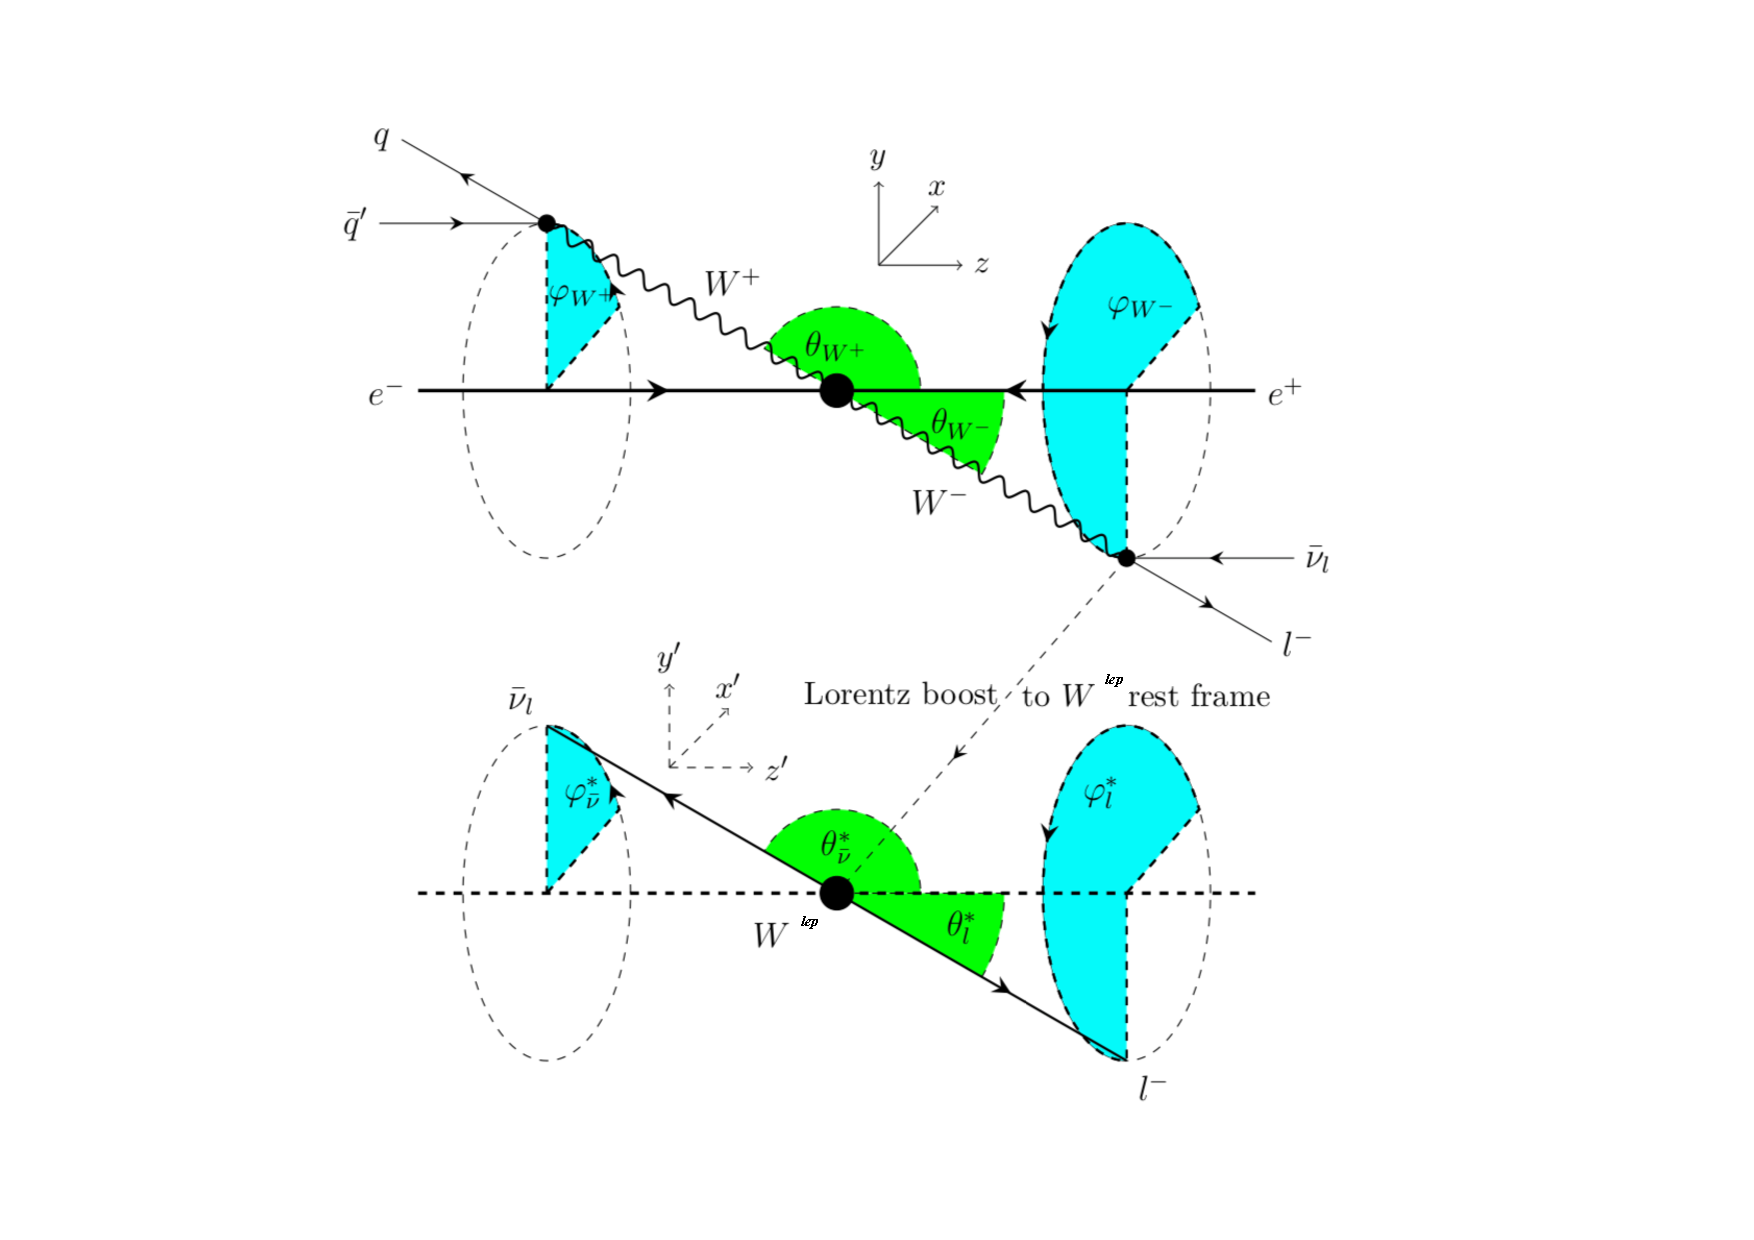
\includegraphics[width=\textwidth]{\imagepath/AngleDiag.pdf}
        \\
        \footnotesize(Modified from Robert Karl 2019)
    \end{minipage}
    \begin{minipage}{0.49\textwidth}
        \resizebox{\linewidth}{!}{%
        \centering
        \begin{tikzpicture}
  \begin{feynman}[scale=1] % using the vertex in brackets () allows fixing of vertex
    \vertex (m) at (-1, 0);
    \vertex (n) at (0.5, 0);
    \vertex (a) at (-1.5,-1);s
    \vertex (b) at ( 1.75,-1) ;
    \vertex (c) at (-1.5, 1);
    \vertex (d) at ( 1.75, 1) ;
    \vertex (u) at ( 3.5,-1.5) {$\mu^-$};
    \vertex (v) at ( 3.5,-0.5) {$\bar{\nu}_\mu$};
    \vertex (q1) at ( 3.5, 1.5) {$q$};
    \vertex (q2) at ( 3.5, 0.5) {$\bar{q'}$};
    \vertex (i1) at (-3,-1) {$e^-$};
    \vertex (i2) at (-3, 1) {$e^+$};
    \diagram* {
      (i1) -- [fermion] (m) ,
      (i2) -- [anti fermion] (m) ,
      (m) -- [photon, edge label=$Z/\gamma$] (n),
      (b) -- [photon, edge label=$W^-$, swap] (n),
      (d) -- [photon, edge label=$W^+$] (n),
      (b) -- [fermion] (u),
      (b) -- [anti fermion] (v),
      (d) -- [fermion] (q1),
      (d) -- [anti fermion] (q2),
    };
  \end{feynman}
\end{tikzpicture}

        }
        \bigskip
        \centering
        \begin{tikzpicture}
  \begin{feynman}[scale=1] % using the vertex in brackets () allows fixing of vertex
    \vertex (n) at (0, 0.75) ;
    \vertex (m) at (0, -0.75) ;
    \vertex (a) at (-1,-1) ;
    \vertex (b) at ( 1.25,-1) ;
    \vertex (c) at (-1, 1);
    \vertex (d) at ( 1.25, 1) ;
    \vertex (u) at ( 3,-1.5) {$\mu^-$};
    \vertex (v) at ( 3,-0.5) {$\bar{\nu}_\mu$};
    \vertex (q1) at ( 3, 1.5) {$q$};
    \vertex (q2) at ( 3, 0.5) {$\bar{q'}$};
    \vertex (i1) at (-2.5,-1) {$e^-$};
    \vertex (i2) at (-2.5, 1) {$e^+$};
    \diagram* {
      (i1) -- [fermion] (m) -- [fermion, edge label=$\nu_e$] (n),
      (i2) -- [anti fermion] (n),
      (b) -- [photon, edge label=$W^-$, swap] (m),
      (d) -- [photon, edge label=$W^+$] (n),
      (b) -- [fermion] (u),
      (b) -- [anti fermion] (v),
      (d) -- [fermion] (q1),
      (d) -- [anti fermion] (q2),
    };
  \end{feynman}
\end{tikzpicture}

    \end{minipage}

\end{frame}

% ----------------------------------------------------------------------------

\begin{frame}\frametitle{Angle Extractions \OrangeBF{Consistent with previous results}}

    \begin{minipage}{0.32\textwidth}
        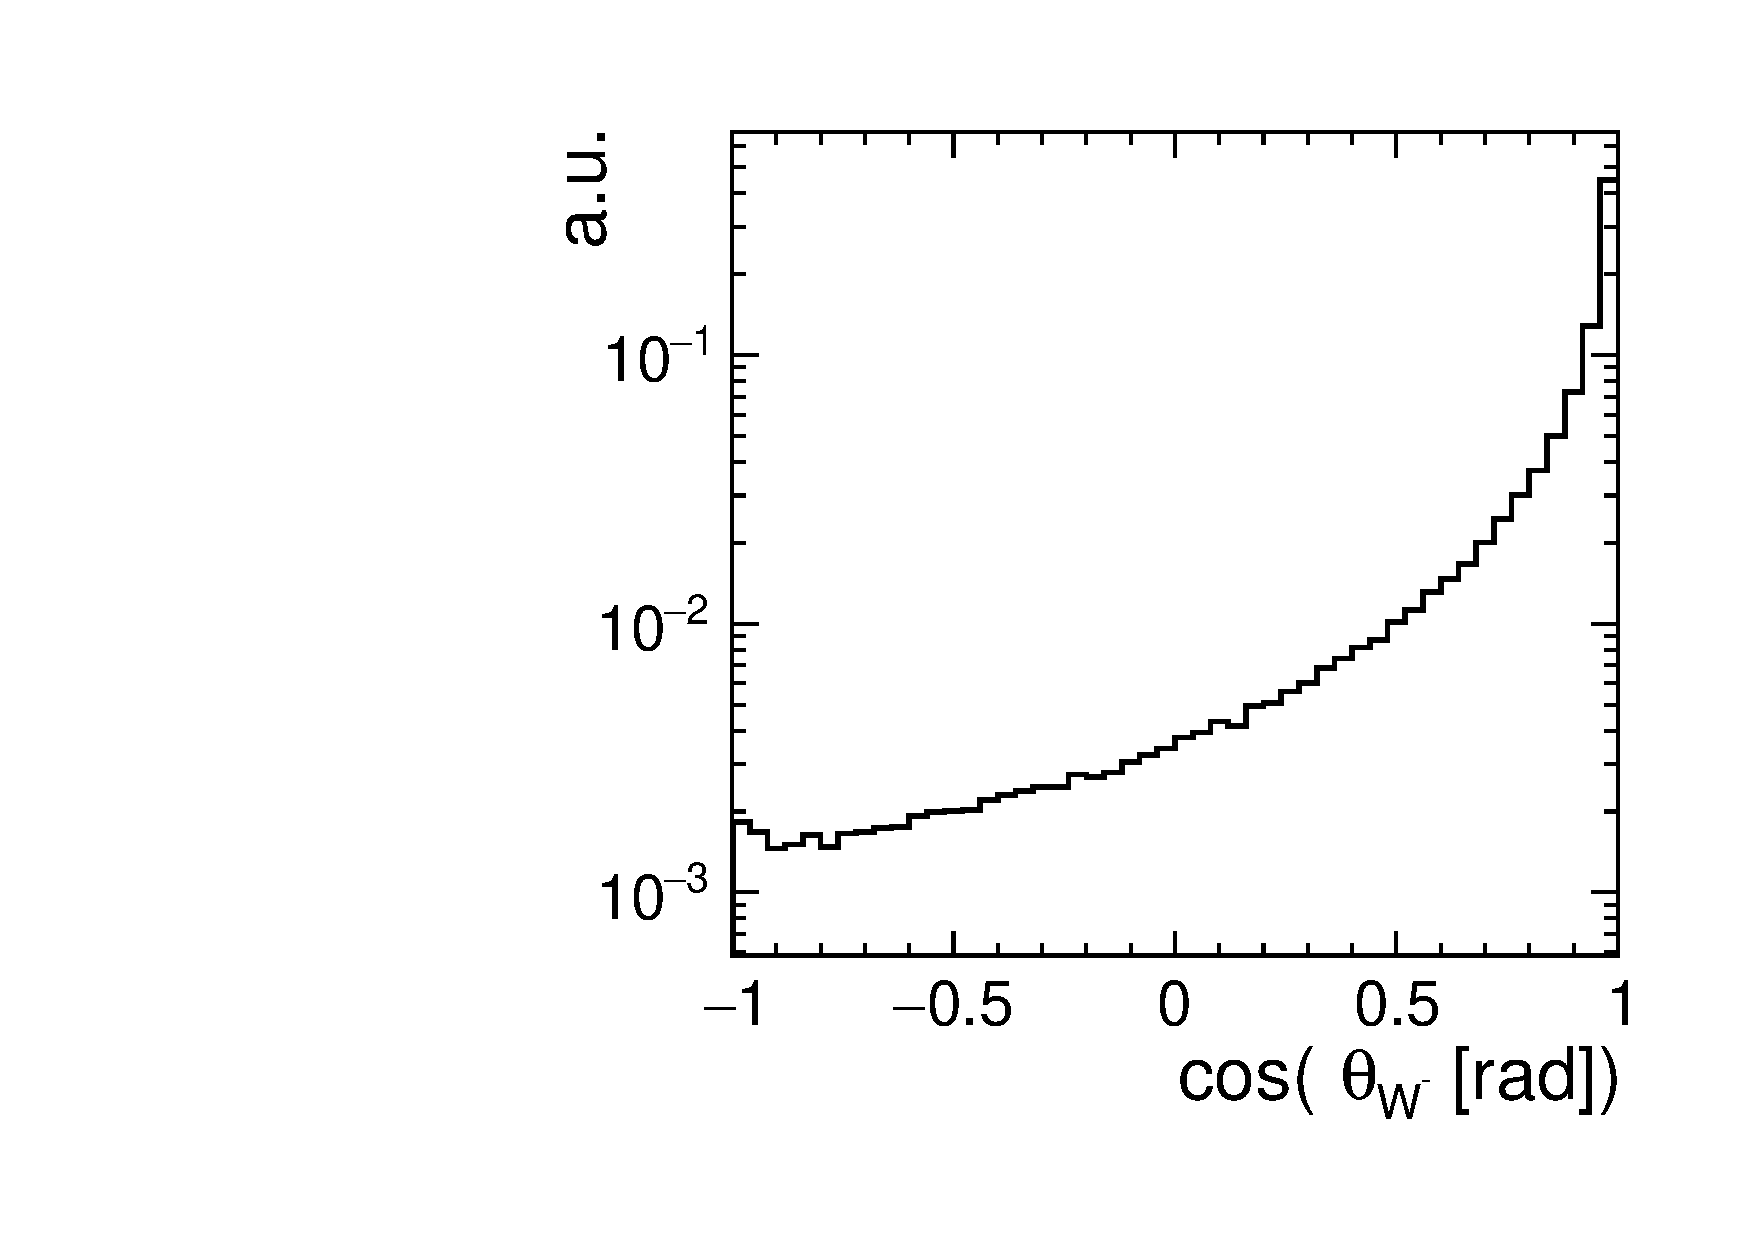
\includegraphics[width=\textwidth]{\imagepath/ThetaMin_cos.pdf}
        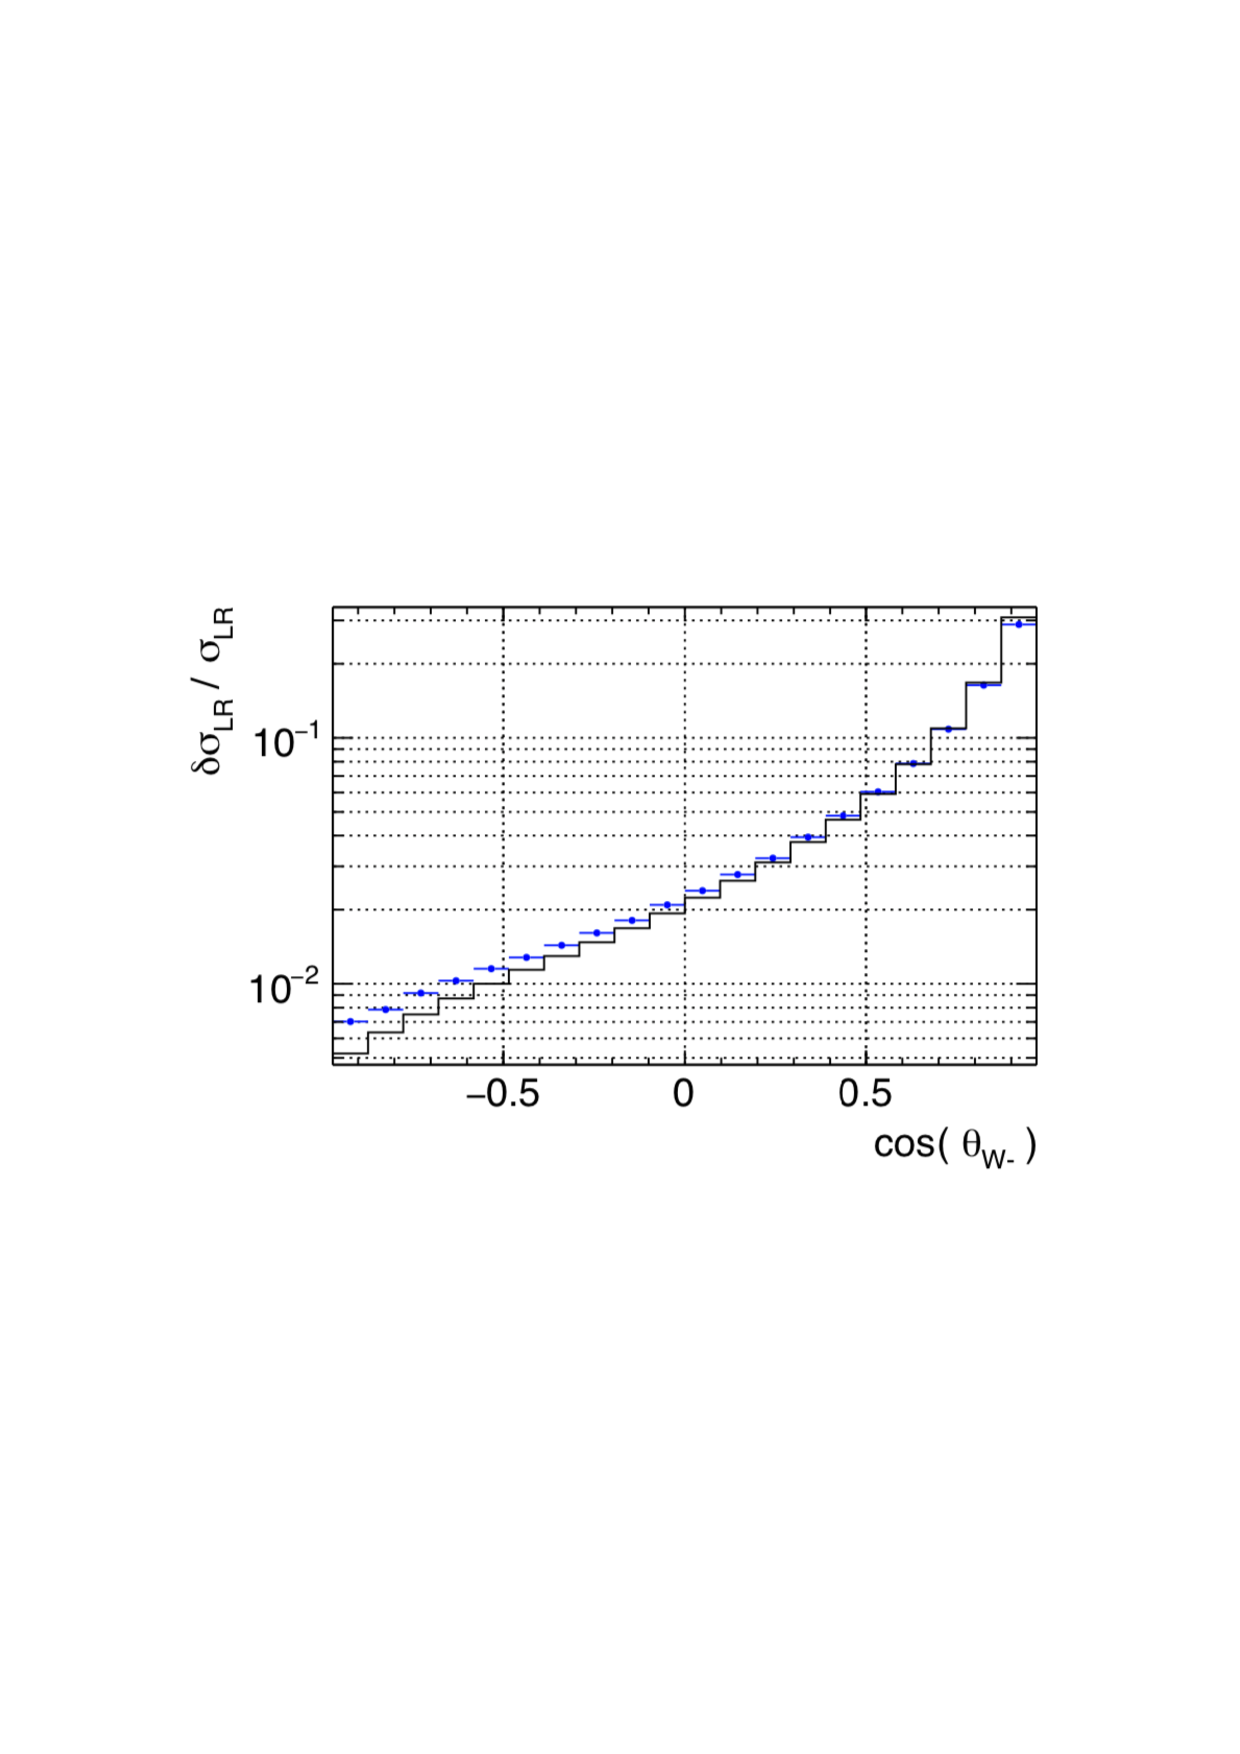
\includegraphics[width=\textwidth]{\imagepath/R_ThetaMin_cos.pdf}
    \end{minipage}\hfill
    \begin{minipage}{0.32\textwidth}
        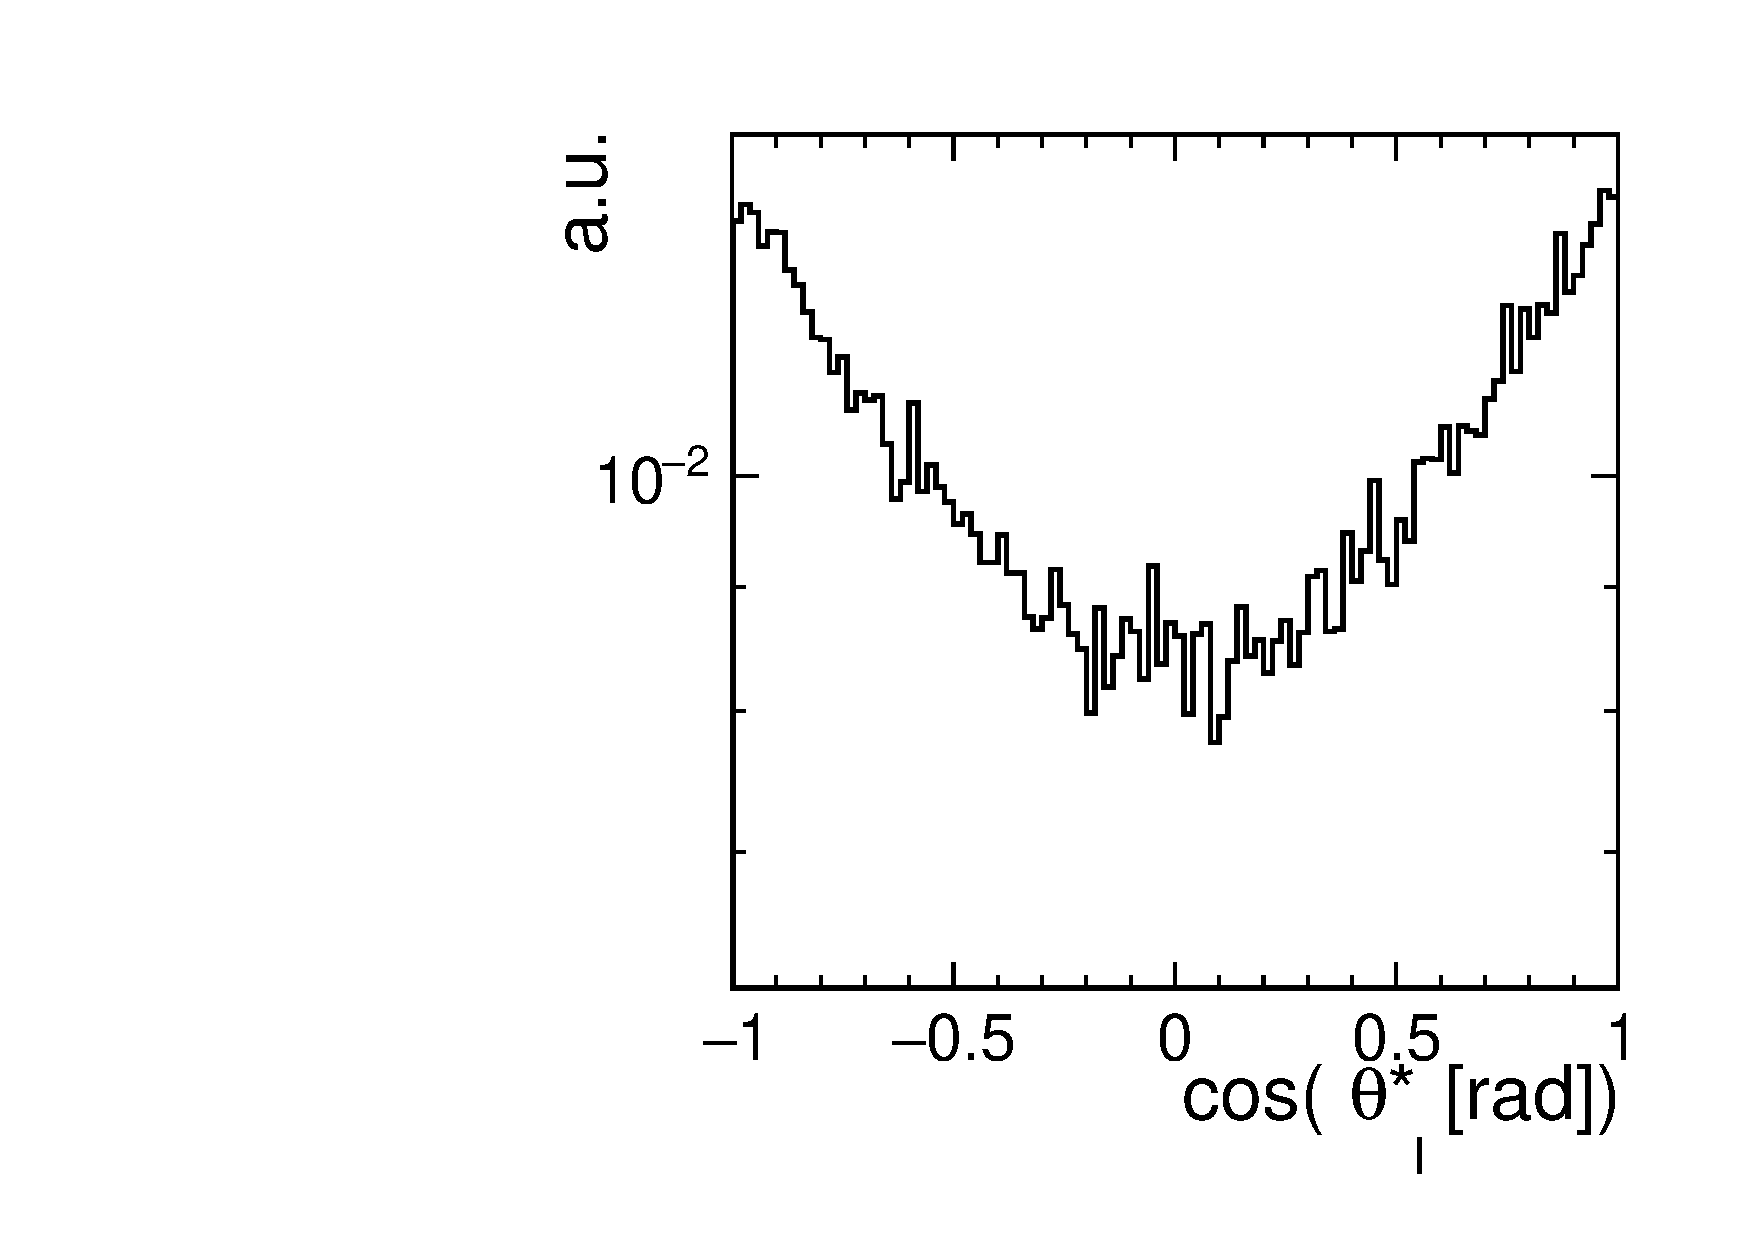
\includegraphics[width=\textwidth]{\imagepath/ThetaLep_cos.pdf}
        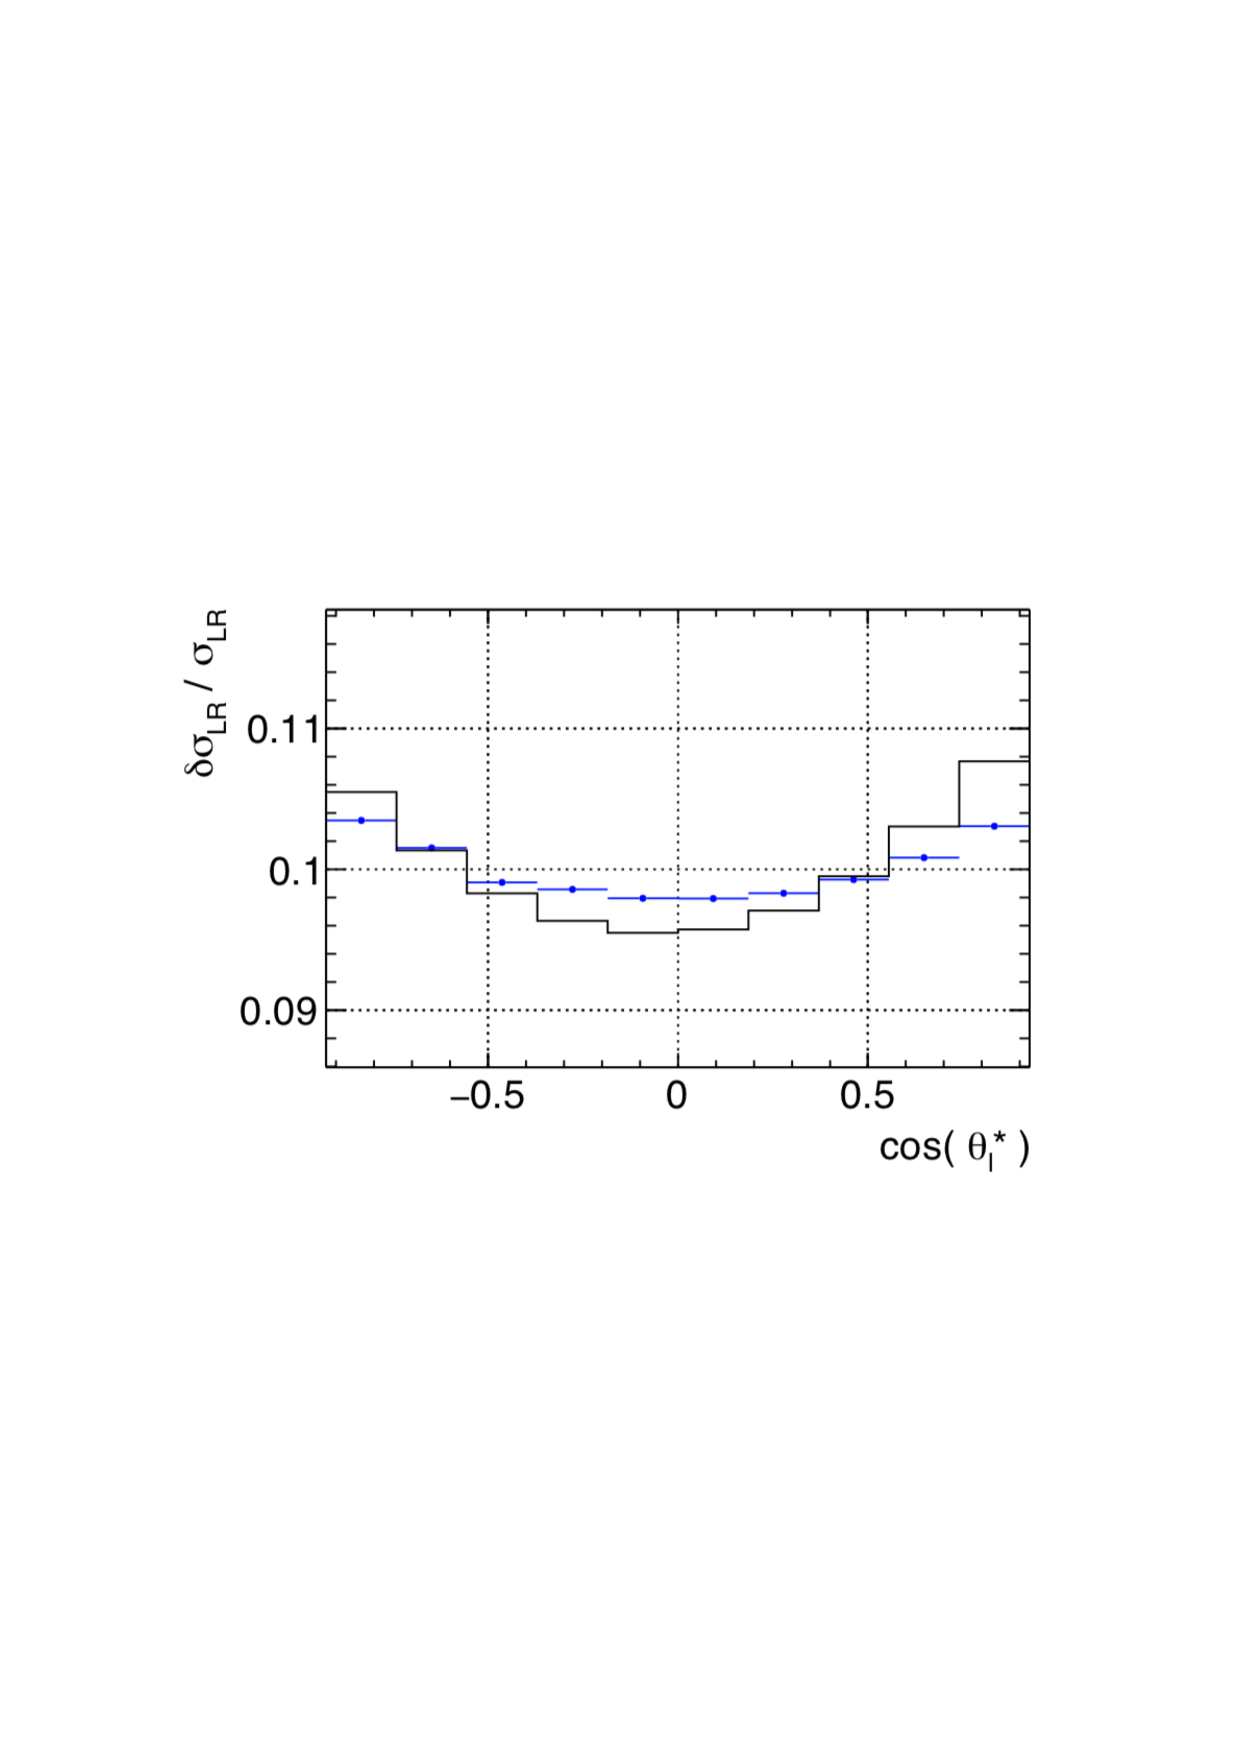
\includegraphics[width=\textwidth]{\imagepath/R_ThetaLep_cos.pdf}
    \end{minipage}
    \begin{minipage}{0.32\textwidth}
        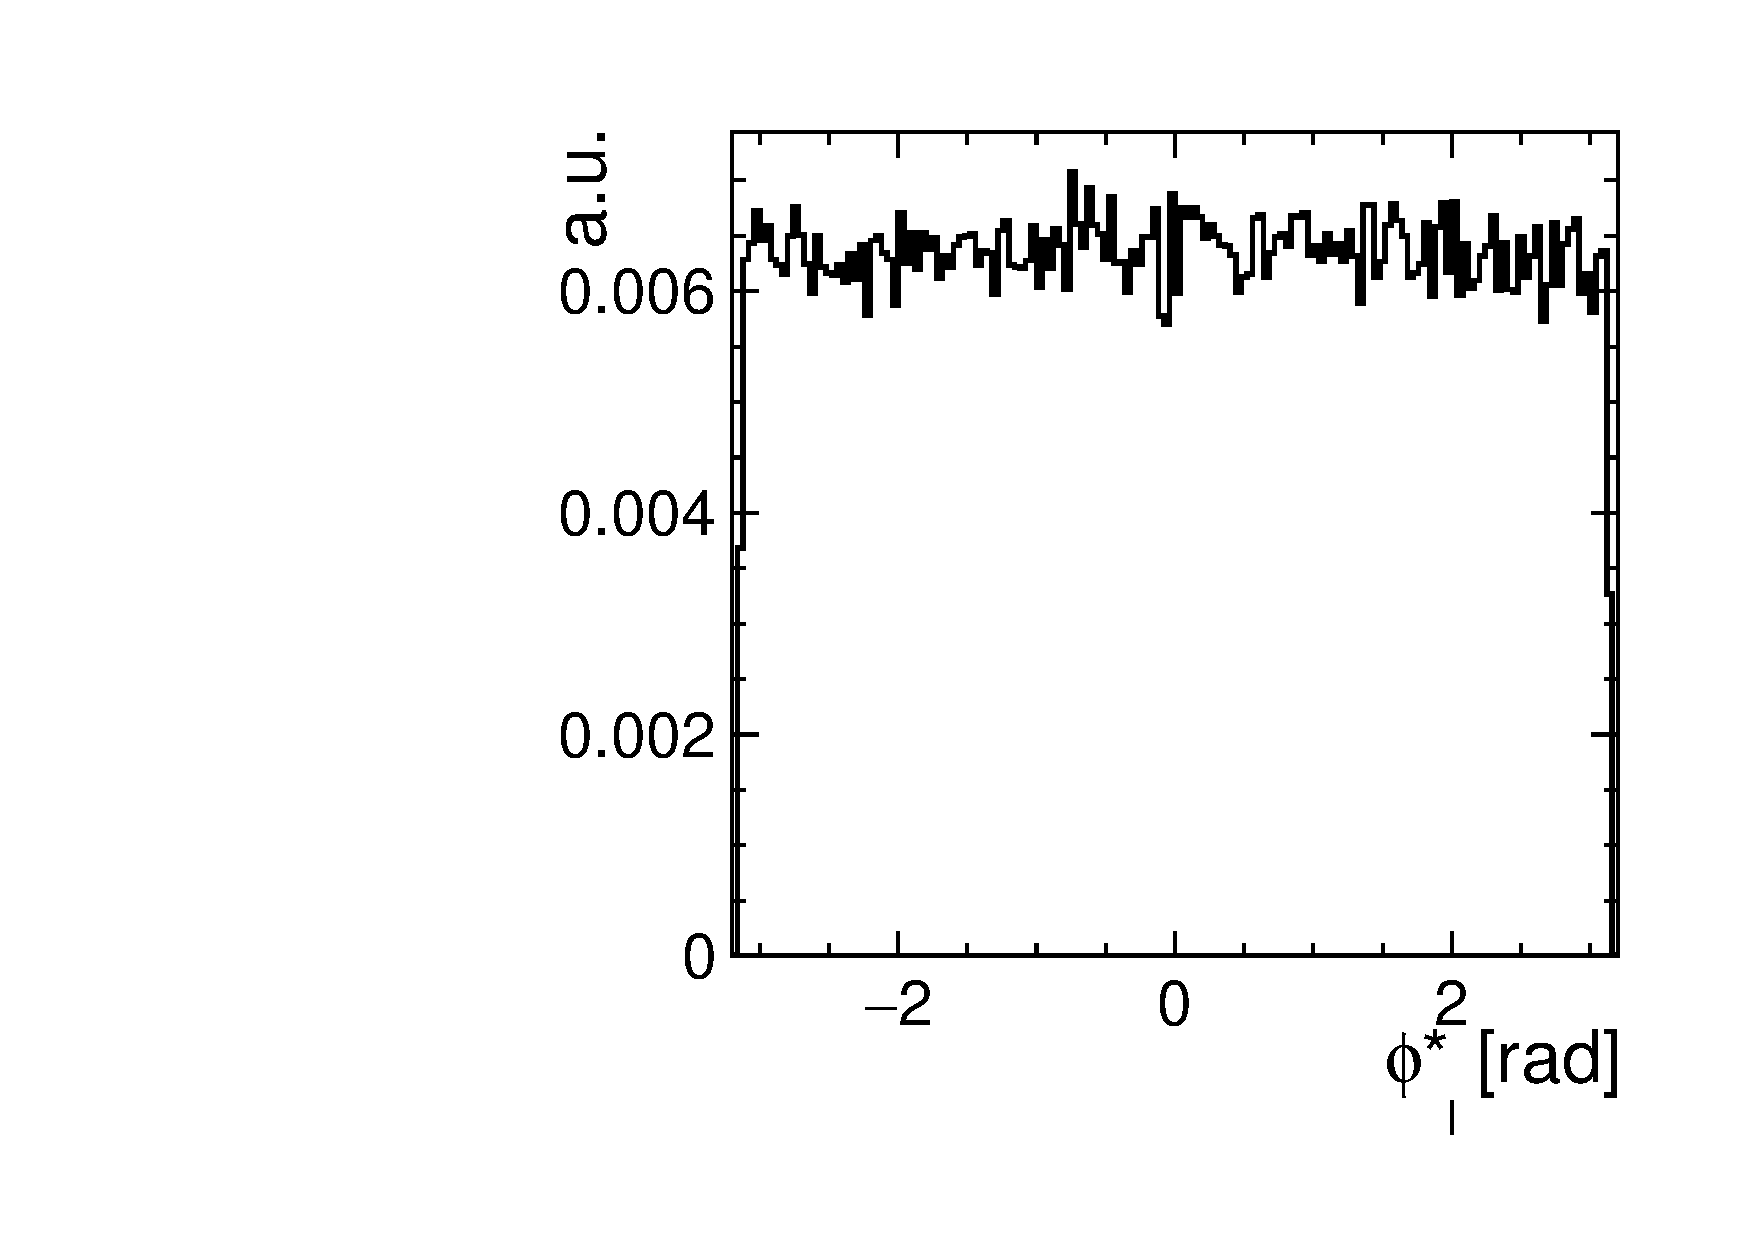
\includegraphics[width=\textwidth]{\imagepath/PhiLep.pdf}
        "it was verified that the ${\phi}_{l}^{*}$ angle distributions are completely flat and yield no information on the chiral structure."
        \\~\\
    \end{minipage}

\end{frame}

% ----------------------------------------------------------------------------

\begin{frame}\frametitle{Angle Efficiencies \OrangeBF{Cut Flow}}

    \centering
    \includegraphics[width=0.9\textwidth, top]{\imagepath/Histflow3_new.pdf}

\end{frame}

% ----------------------------------------------------------------------------

\begin{frame}\frametitle{Angle Efficiencies \OrangeBF{Applying the Cuts}}

    \begin{minipage}{0.32\textwidth}
        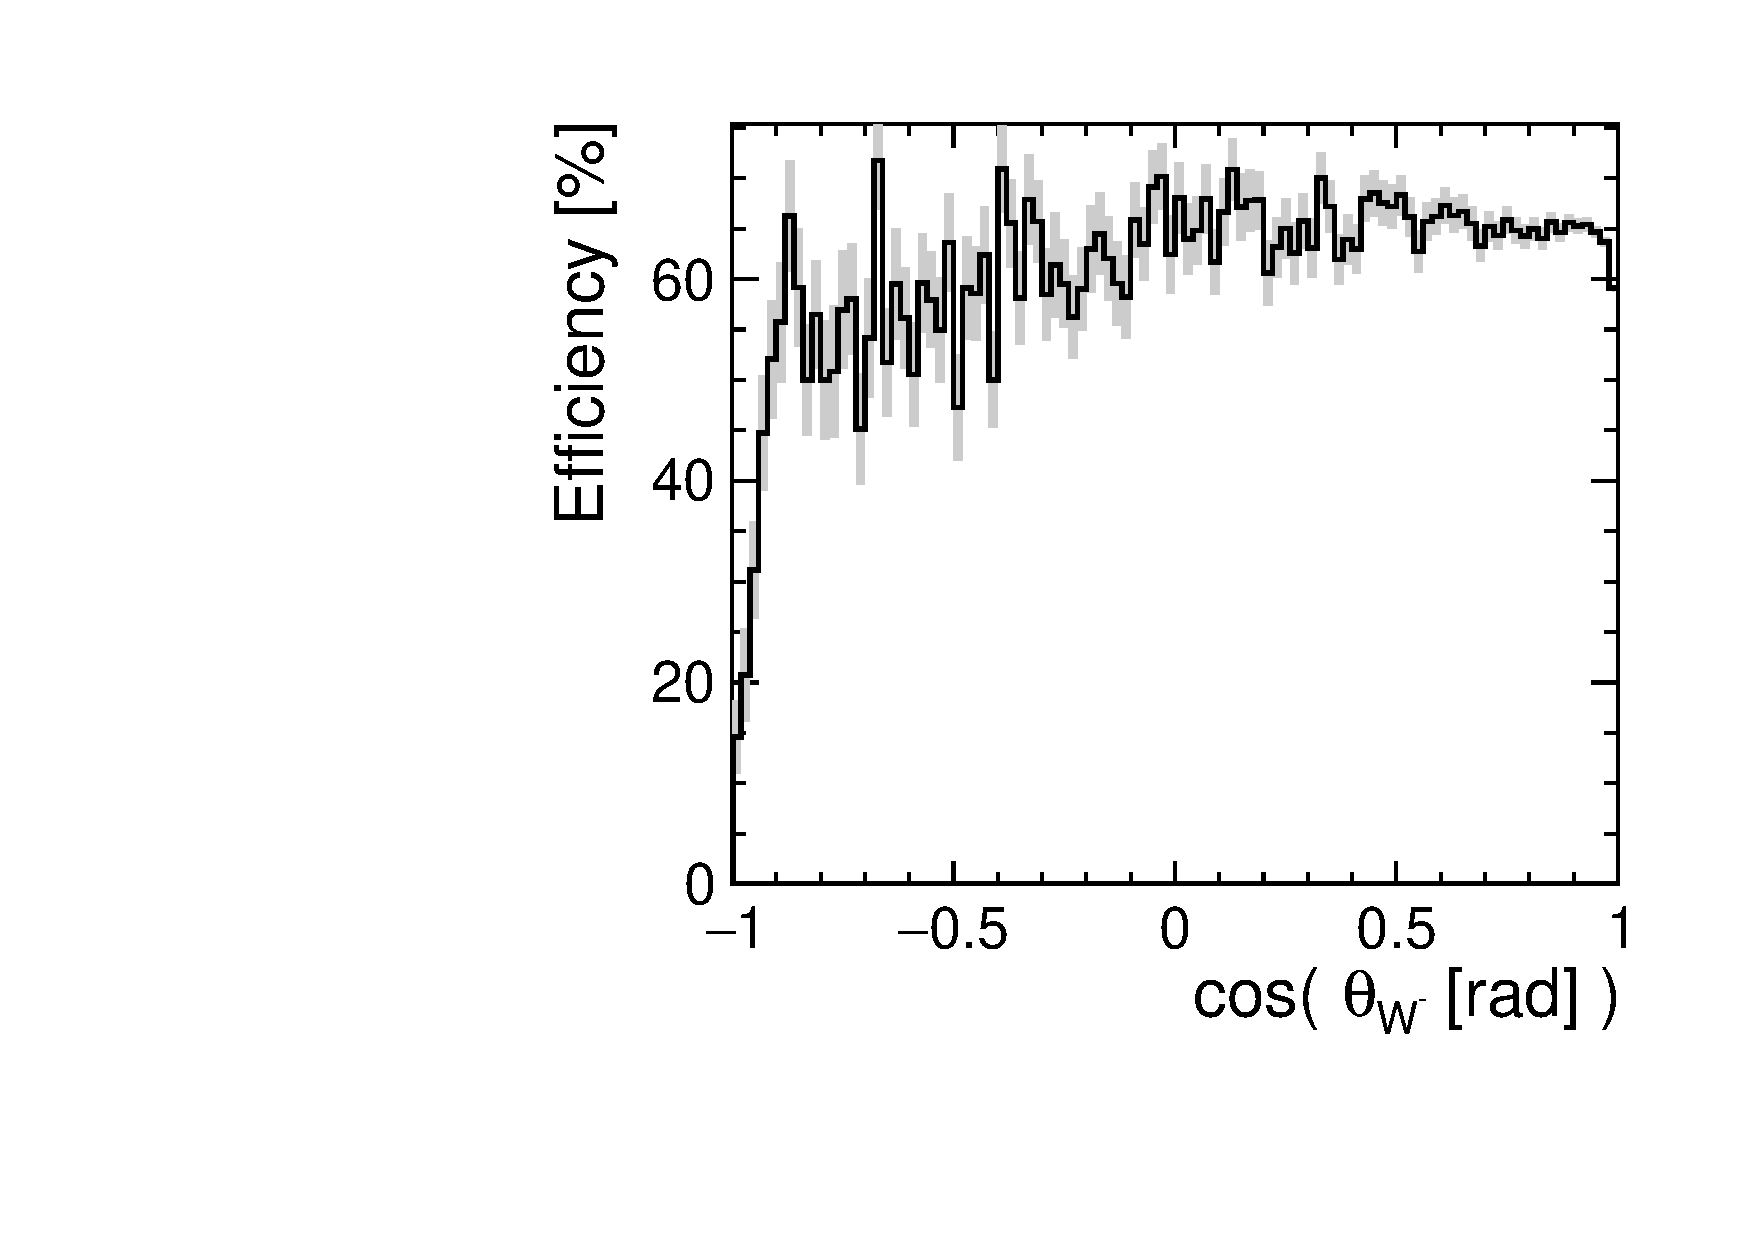
\includegraphics[width=\textwidth]{\imagepath/E_ThetaMin_cos_err.pdf}
        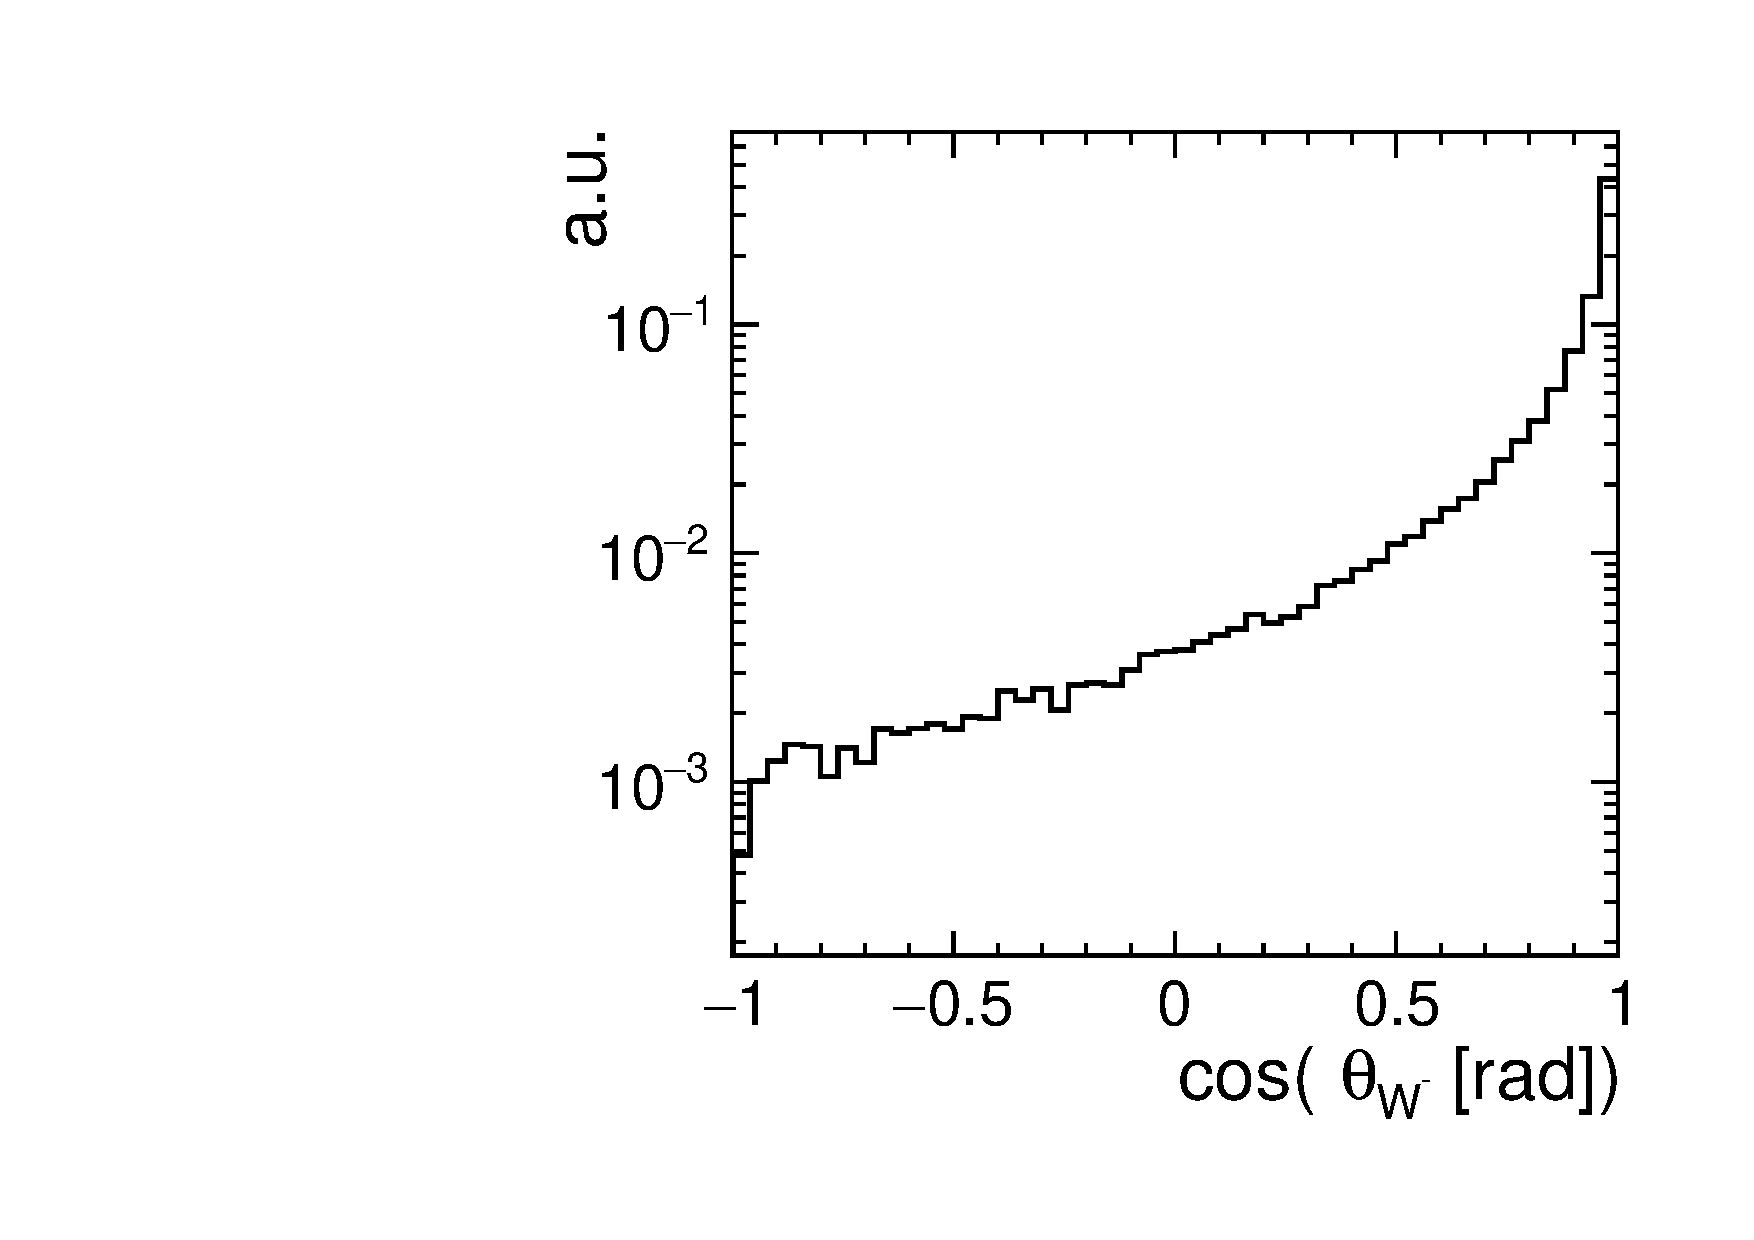
\includegraphics[width=\textwidth]{\imagepath/ThetaMin_cos_cut.pdf}
    \end{minipage}\hfill
    \begin{minipage}{0.32\textwidth}
        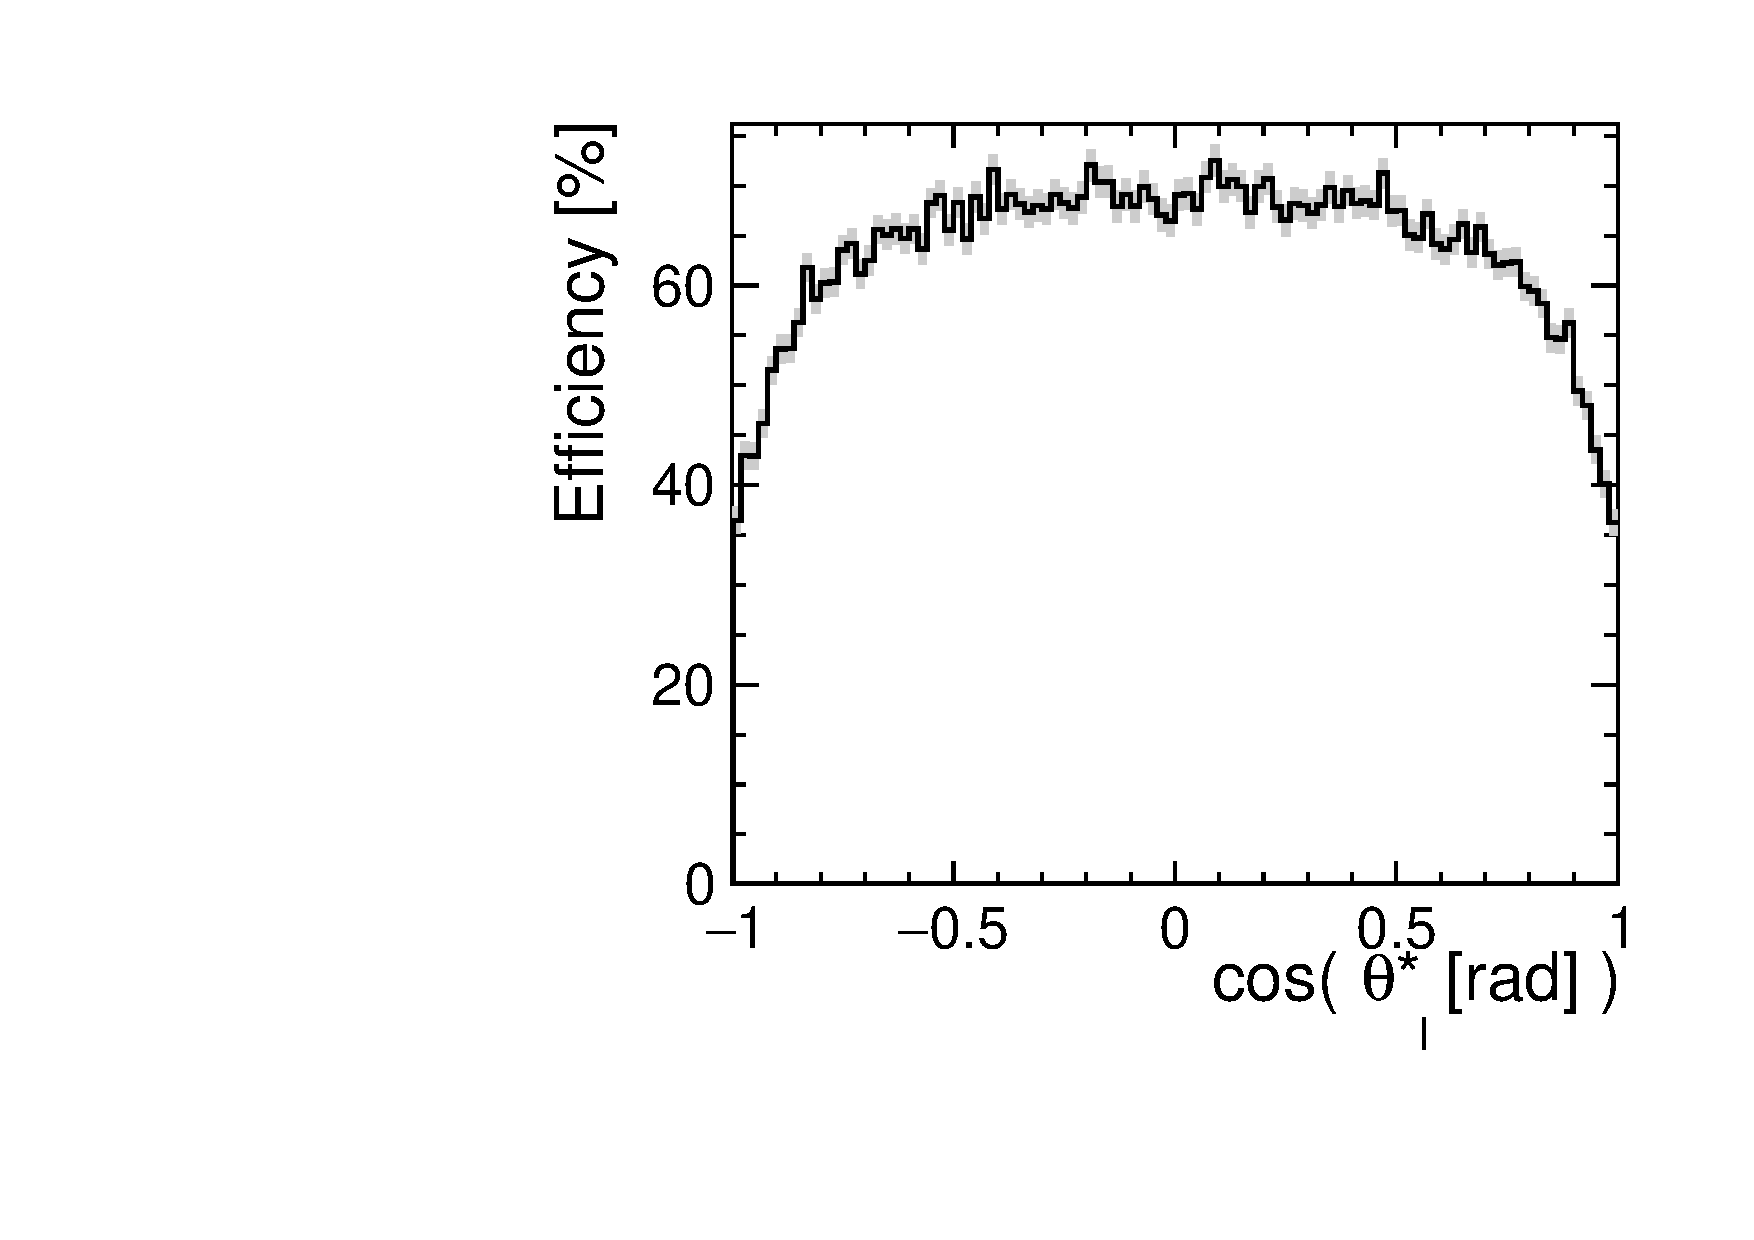
\includegraphics[width=\textwidth]{\imagepath/E_ThetaLep_cos_err.pdf}
        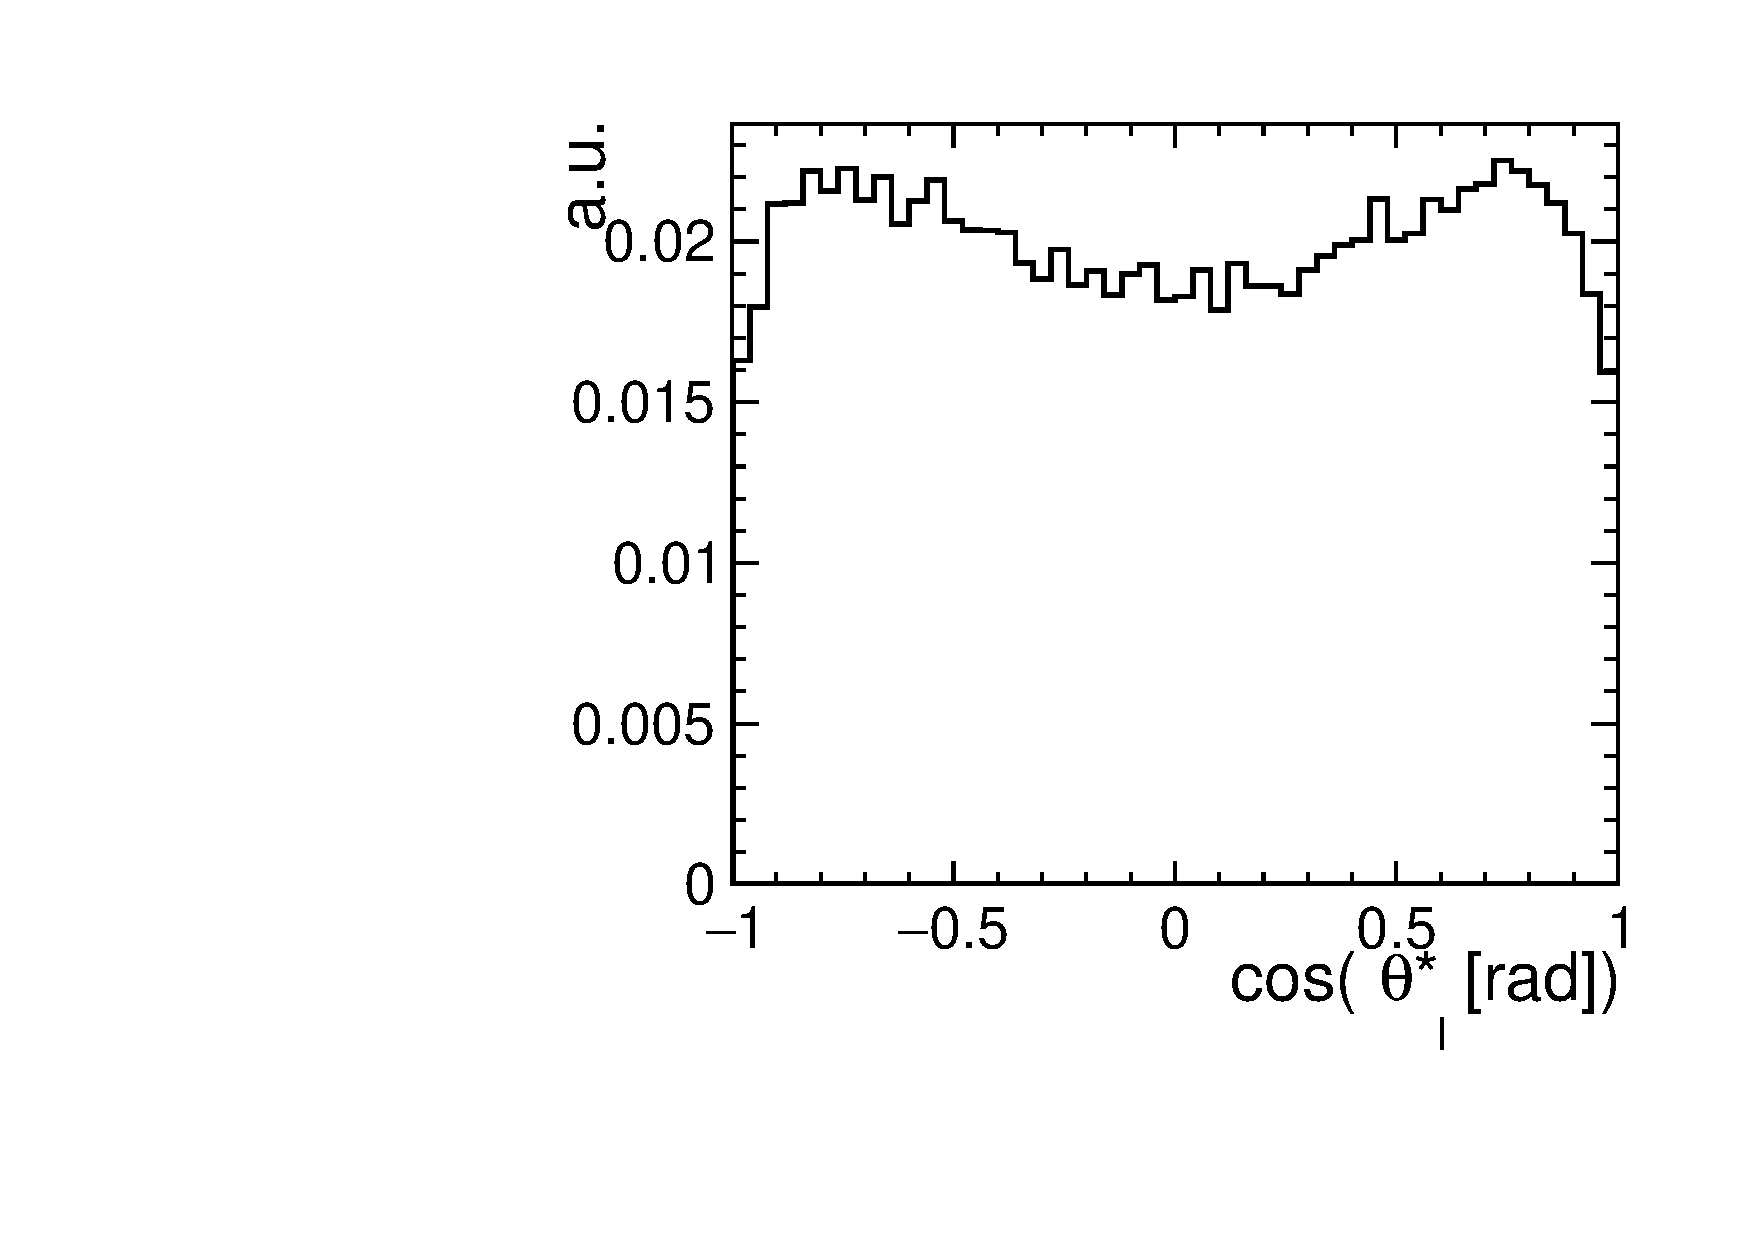
\includegraphics[width=\textwidth]{\imagepath/ThetaLep_cos_cut.pdf}
    \end{minipage}
    \begin{minipage}{0.32\textwidth}
        \includegraphics[width=\textwidth]{\imagepath/E_PhiLep_Err.pdf}
        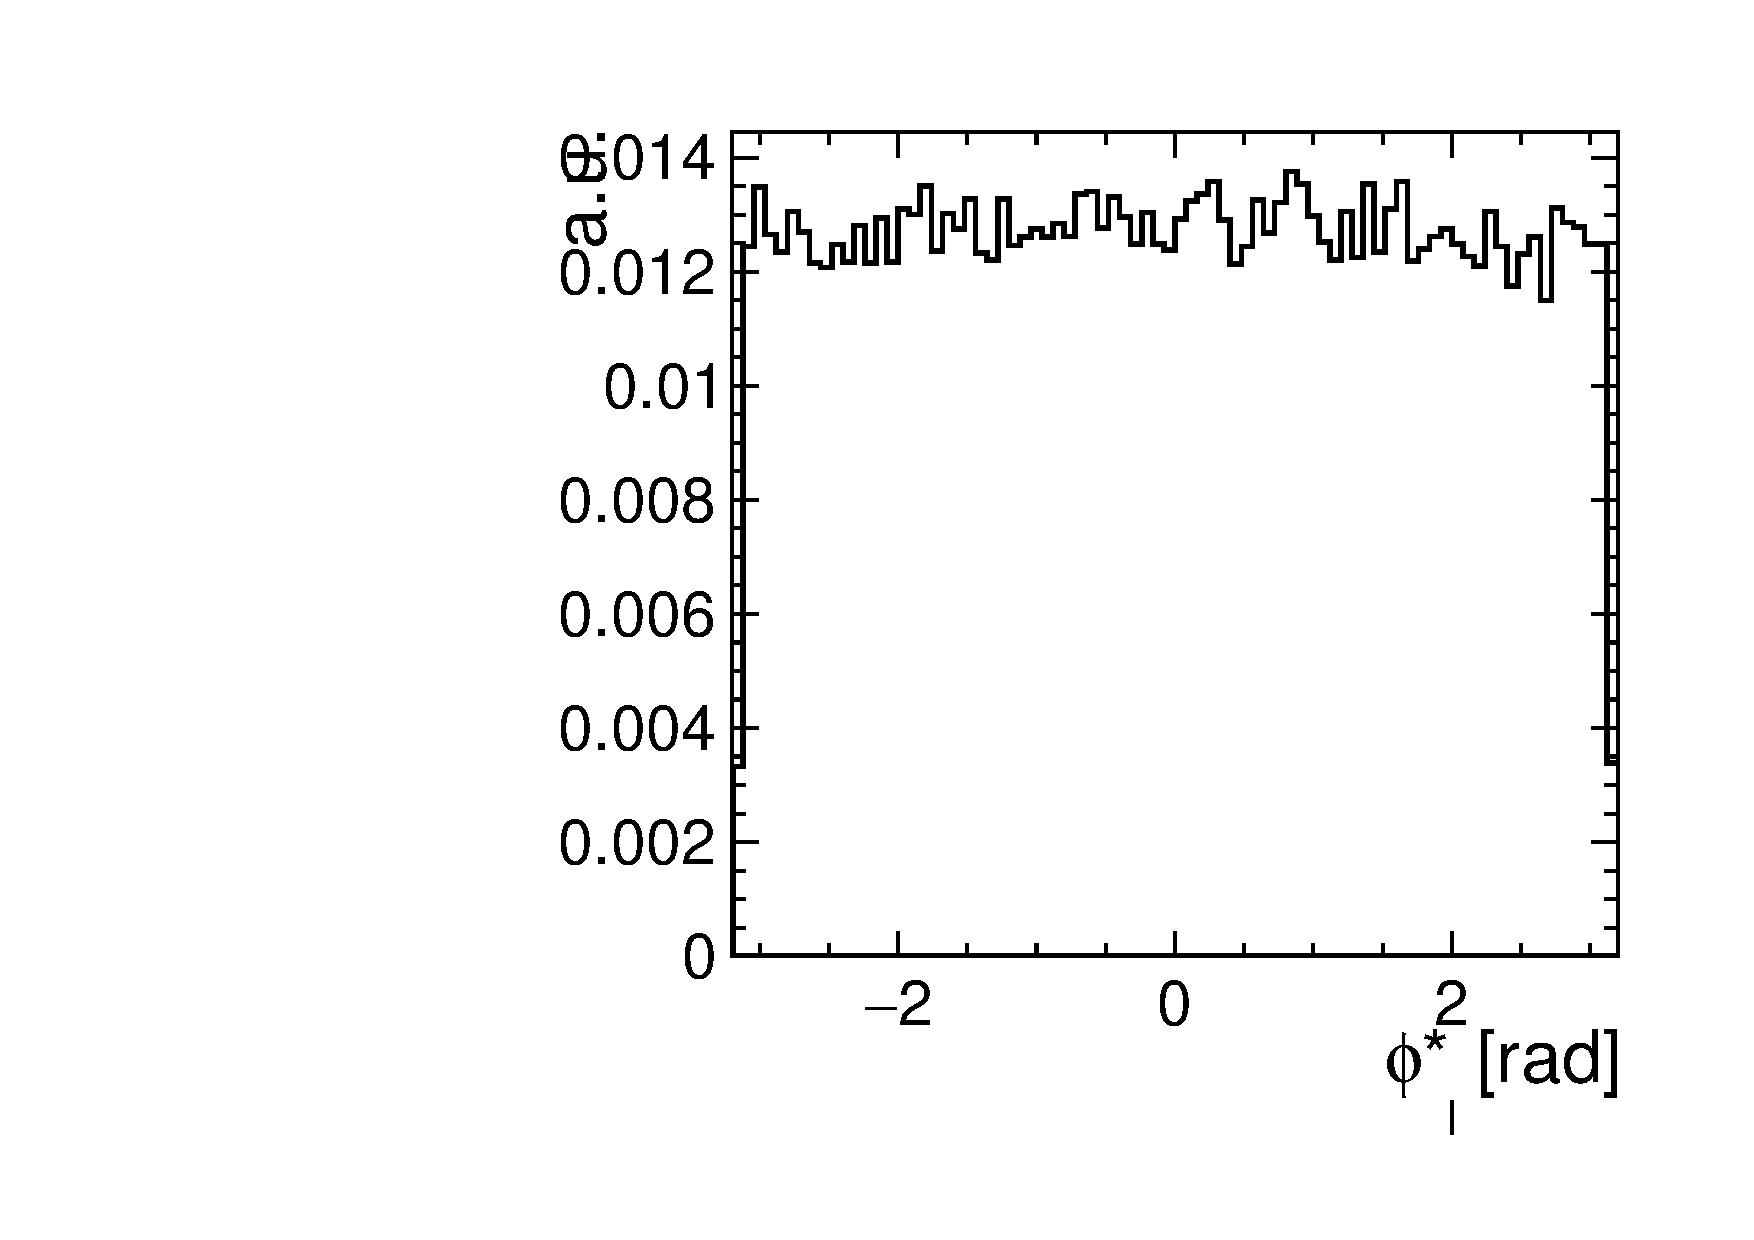
\includegraphics[width=\textwidth]{\imagepath/PhiLep_cut.pdf}
    \end{minipage}
\end{frame}

% ----------------------------------------------------------------------------

\begin{frame}\frametitle{Angle Efficiencies \OrangeBF{${E}_{\gamma} < 1$ GeV}}

    \begin{minipage}{0.32\textwidth}
        \centering
        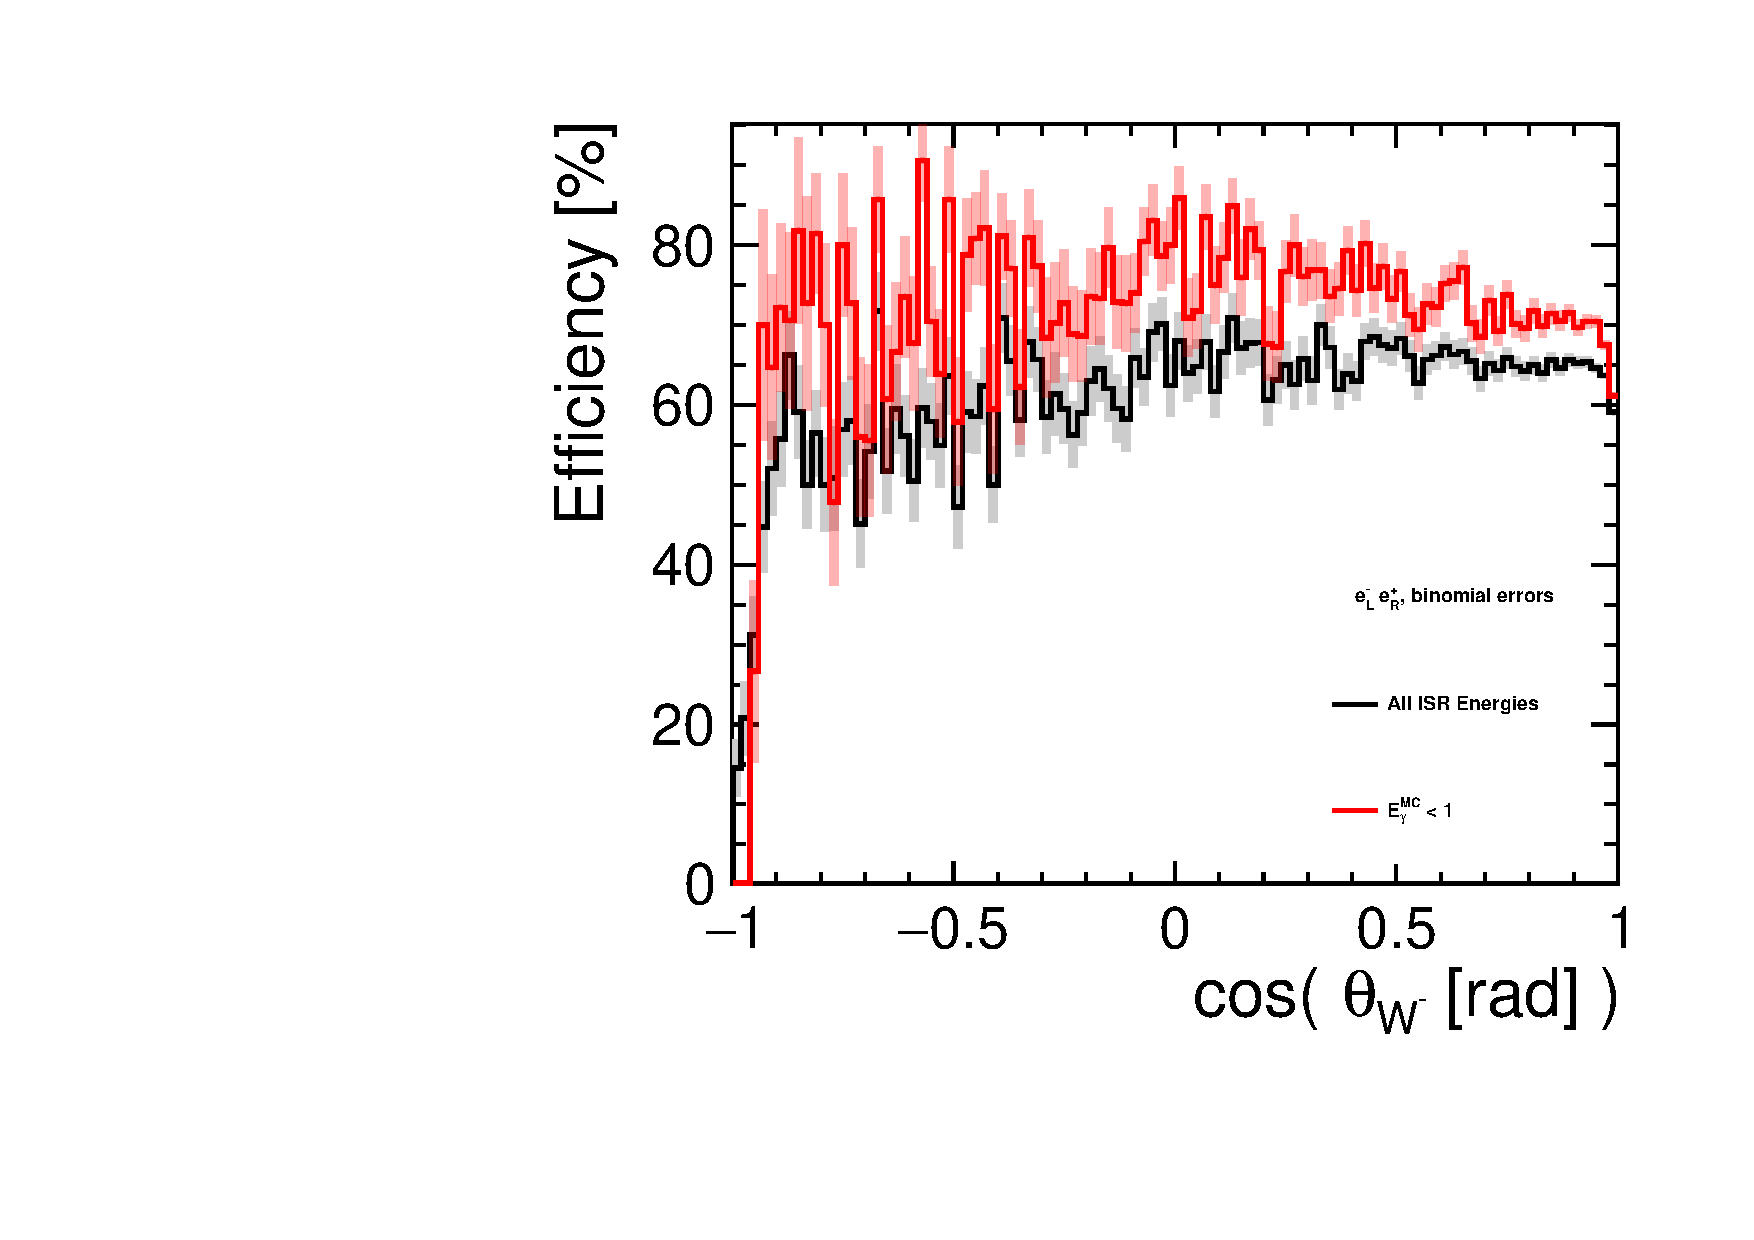
\includegraphics[width=\textwidth]{\imagepath/P_E_ThetaMin_cos_err_Both.pdf}
    \end{minipage}
    \begin{minipage}{0.32\textwidth}
        \centering
        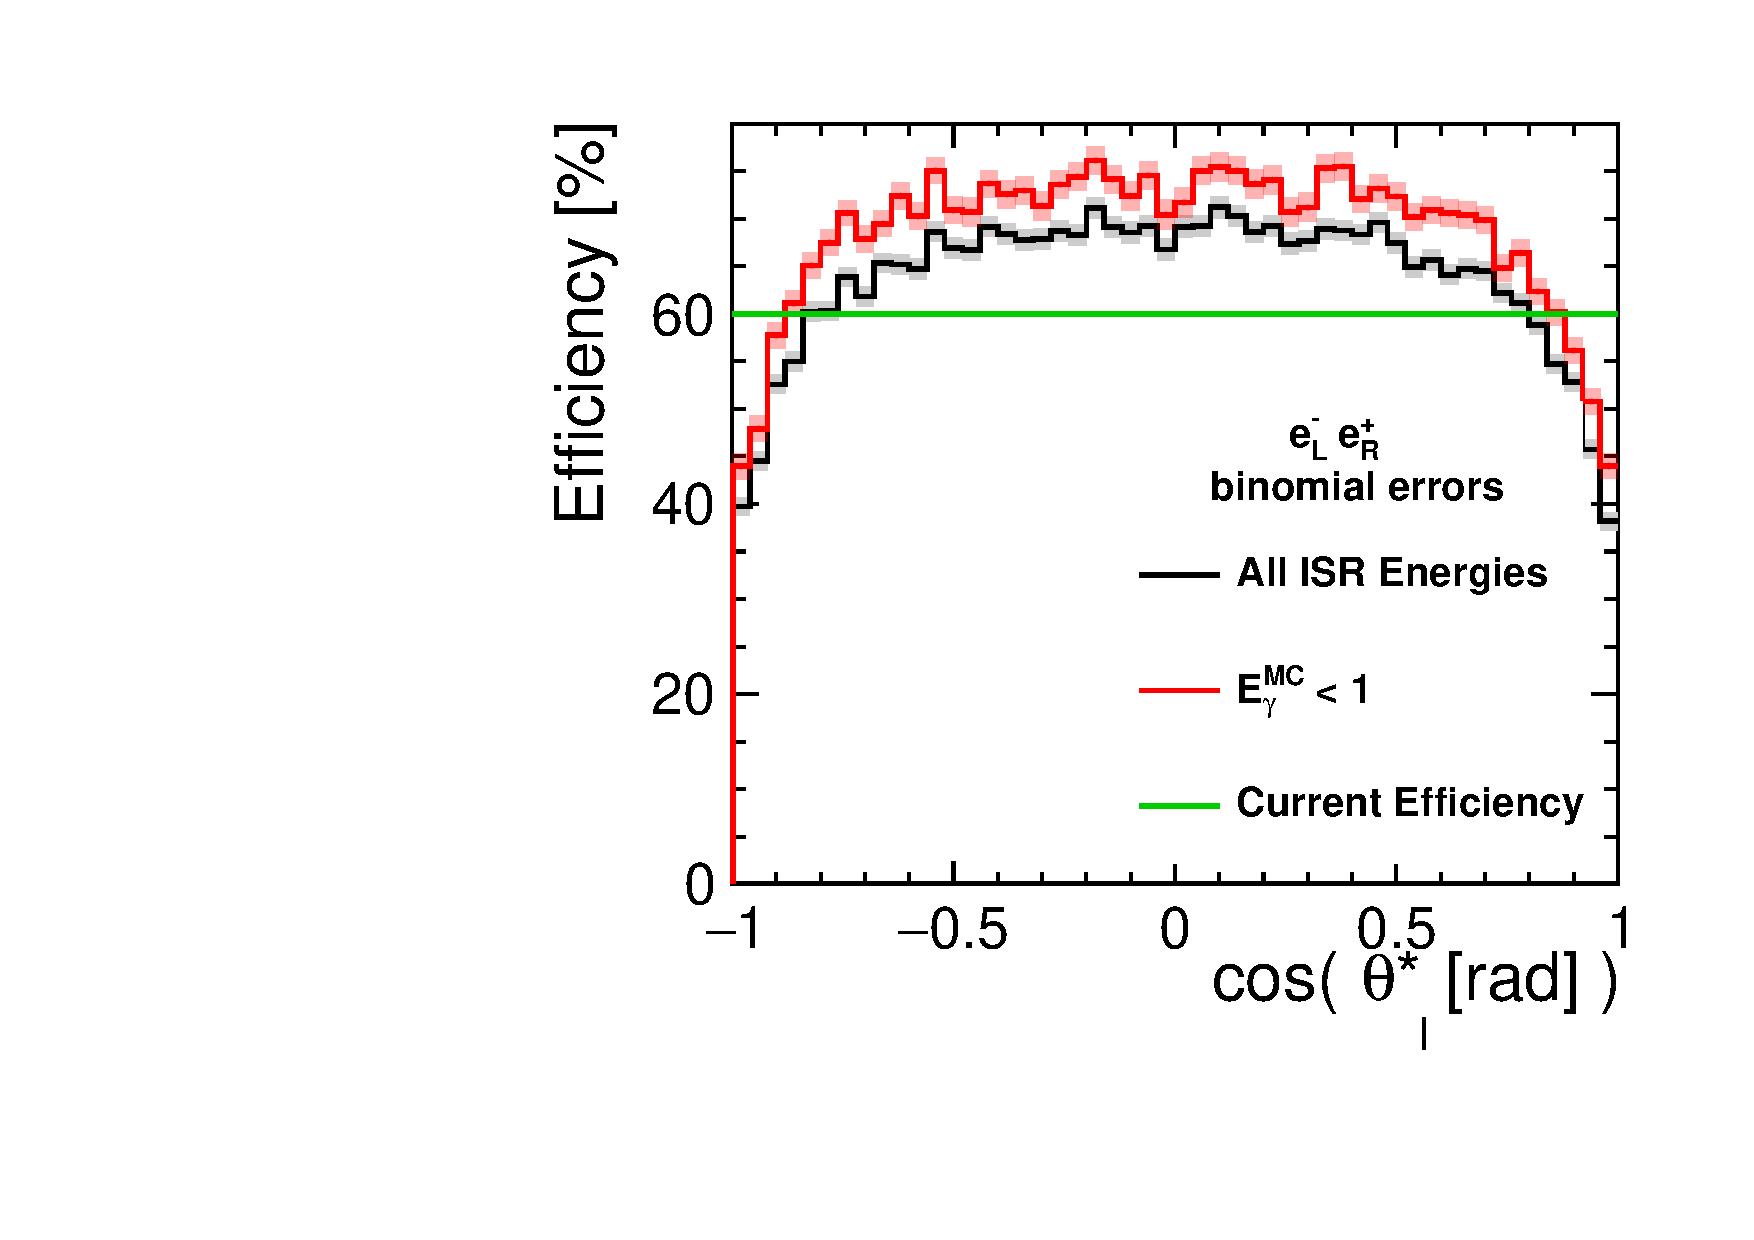
\includegraphics[width=\textwidth]{\imagepath/P_E_ThetaLep_cos_err_Both.pdf}
    \end{minipage}
    \begin{minipage}{0.32\textwidth}
        \centering
        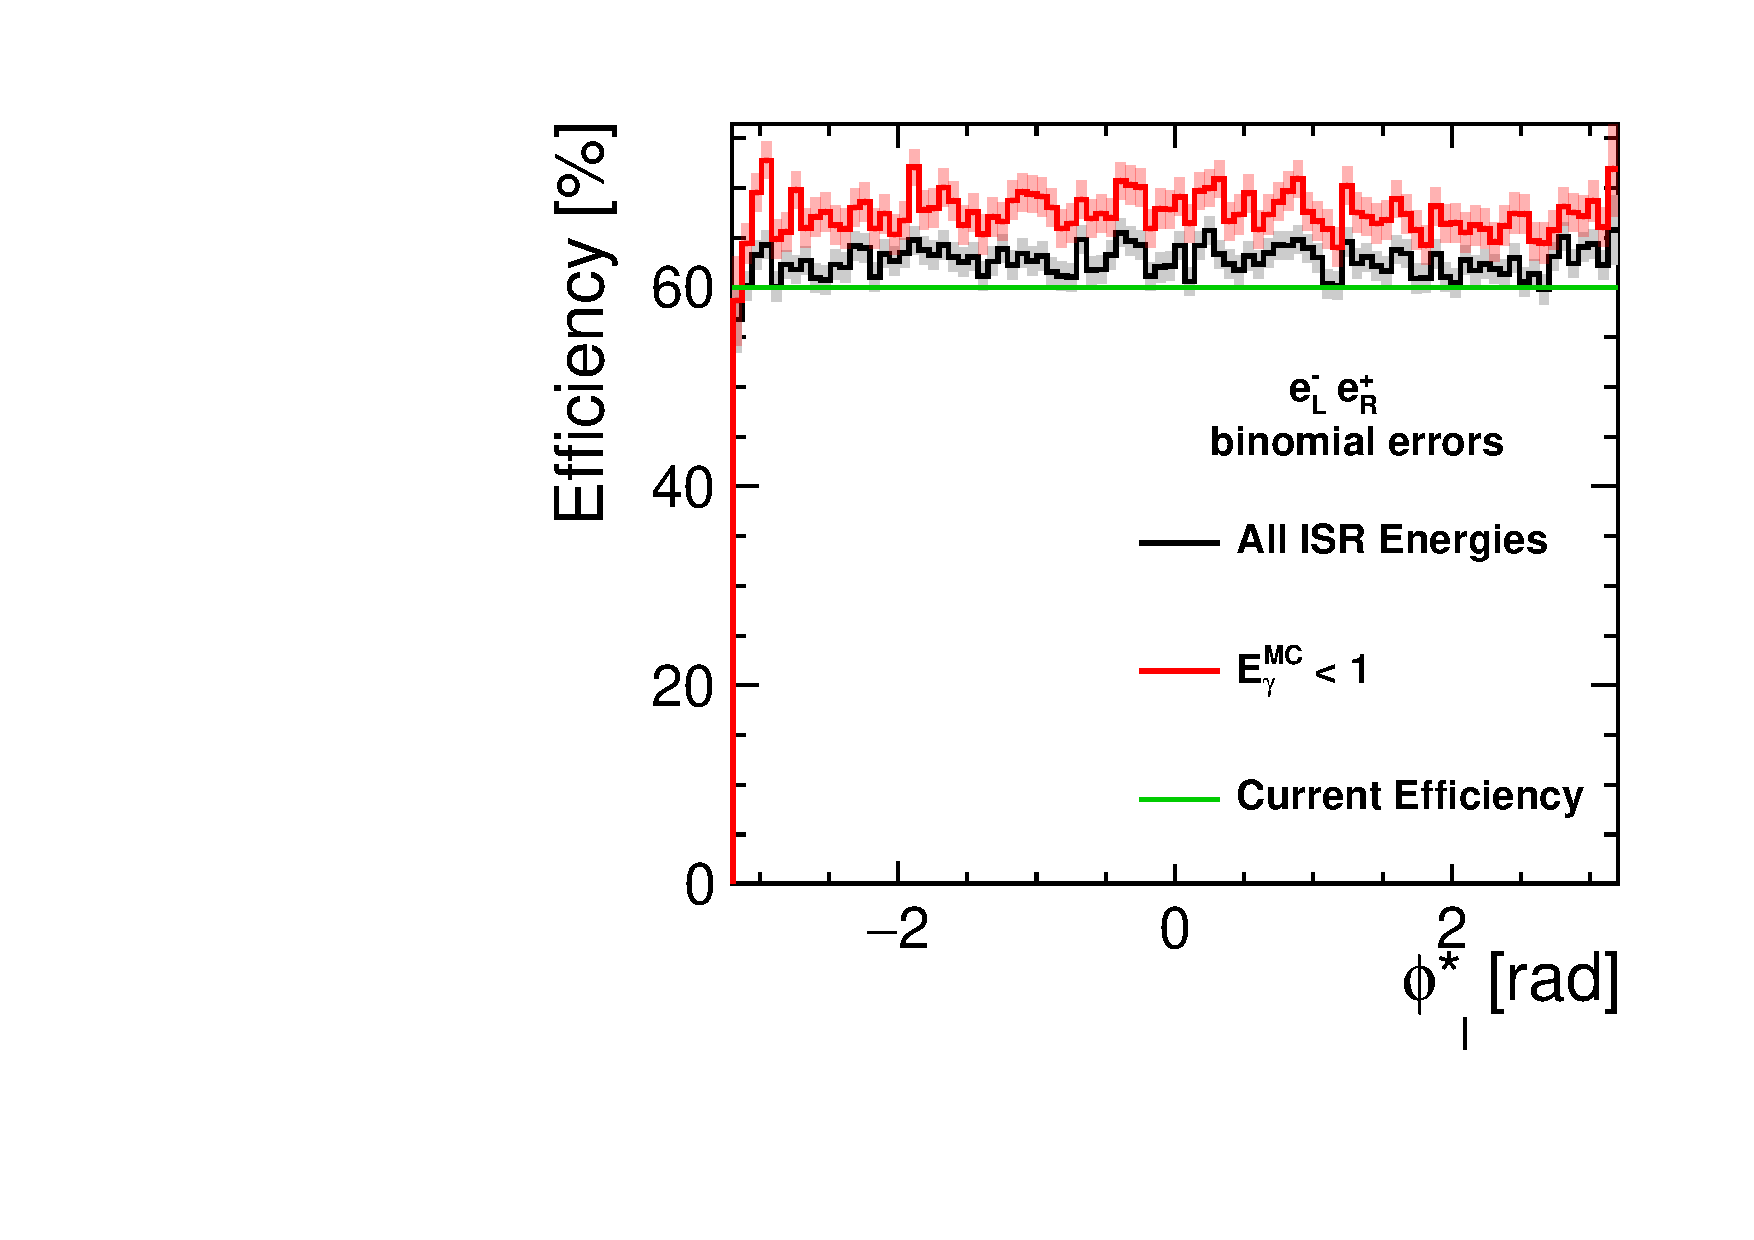
\includegraphics[width=\textwidth]{\imagepath/P_E_PhiLep_err_Both.pdf}
    \end{minipage}

\end{frame}

% ----------------------------------------------------------------------------
% ----------------------------------------------------------------------------
\appendix
% ----------------------------------------------------------------------------
% ----------------------------------------------------------------------------

\begin{frame}\frametitle{Back Up Slides \OrangeBF{Cut Flow table}}

    \begin{table}[!]
    \centering
    \resizebox{0.8\textwidth}{!}{%
        \begin{tabular}{|l|l|l|l|l|l|} \hline
            Order & Cut description & \multicolumn{4}{c|}{Efficiency [\%]} \\ \cline{3-6}
            & & \multicolumn{3}{c|}{My Results} & Ivan's Results \\  \cline{3-5}
            & & n = 2129 & \multicolumn{2}{c|}{n = 99419} & n = 107233 \\ \cline{4-5}
            & & & no cheat & cheat & \\ \hline \hline
            0 & muon signal & 100.00 & 100.00 & 100.00 & 100.00 \\ \hline
            1 & track multiplicity ${n}_{tracks} \ge 10$ & 97.13 & 97.01 & 96.23 & 99.996 \\ \hline
            2 & center of mass energy $\sqrt{s} > 100$ GeV & 92.29 & 91.69 & 84.35 & 97.96 \\ \hline
            3 & total transverse momentum ${P}_{T} > 5$ GeV & 91.16 & 90.47 & 83.28 & 96.69 \\ \hline
            4 & total energy ${E}_{SUM} < 500$ GeV & 89.66 & 89.28 & 82.70 & 95.36 \\ \hline
            5 & $\ln{({y}_{+})} \in [-12, -3]$ (*) & 88.69 & 88.08 & 82.47 & 95.01 \\ \hline
            6 & 1 lepton found (*) & 80.65 & 80.77 & 81.50 & 78.75 \\ \hline
            7 & pre ISR correction ${m}_{W}^{lep} \in [20, 250]$ GeV &  78.23 & 77.94 & 77.84 & 76.61 \\ \hline
            8 & tau discrimination &  76.05 & 75.60 & 75.73 & 74.07 \\ \hline
            9 & charged lepton (*) & 76.05 & 75.60 & 75.73 & 73.51 \\ \hline
            10 & isolation variable ${\Delta\Omega}_{iso} > 0.5$ & 76.01 & 75.58 & 75.72 & 73.42 \\ \hline
            11 & post ISR correction ${m}_{W}^{lep} \in [40, 120]$ GeV & 72.90 & 72.77 & 72.33 & 70.13 \\ \hline
            12 & post ISR correction ${m}_{W}^{had} \in [40, 120]$ GeV & 63.21 & 62.92 & 70.52 & 66.93 \\ \hline
            13 & $\cos{{\theta}_{W}} > -0.95$ & 63.02 & 62.65 & 70.21 & 66.78 \\ \hline
        \end{tabular}
    }
    \end{table}

    \end{frame}

% ----------------------------------------------------------------------------

\begin{frame}\frametitle{Back Up Slides \OrangeBF{Cut definitions}}

    \begin{itemize}
        \item $\Delta{\Omega}_{iso}$ defined as,
            \begin{align}
                 ({\phi}_{lep} - {\phi}_{had}) < \pi \to \Delta{\Omega}_{iso} &= \sqrt{{({\theta}_{lep} - {\theta}_{had})}^{2}+{({\phi}_{lep} - {\phi}_{had})}^{2}} \\
                 ({\phi}_{lep} - {\phi}_{had}) \ge \pi \to \Delta{\Omega}_{iso} &= \sqrt{{({\theta}_{lep} - {\theta}_{had})}^{2} + {(2\pi - |{\phi}_{lep} - {\phi}_{had} |)}^{2}} \, .
            \end{align}
        \item ${\tau}_{discr}$ defined by
            \begin{align}
                {\tau}_{discr} = {(\frac{2{E}_{lep}}{\sqrt{s}})}^{2} + {(\frac{{m}_{W}^{lep}}{{m}_{W}^{true}})}^{2}
            \end{align}
    \end{itemize}
\end{frame}

% ----------------------------------------------------------------------------

\begin{frame}\frametitle{Back Up Slides \OrangeBF{Number of Isolated leptons found}}

    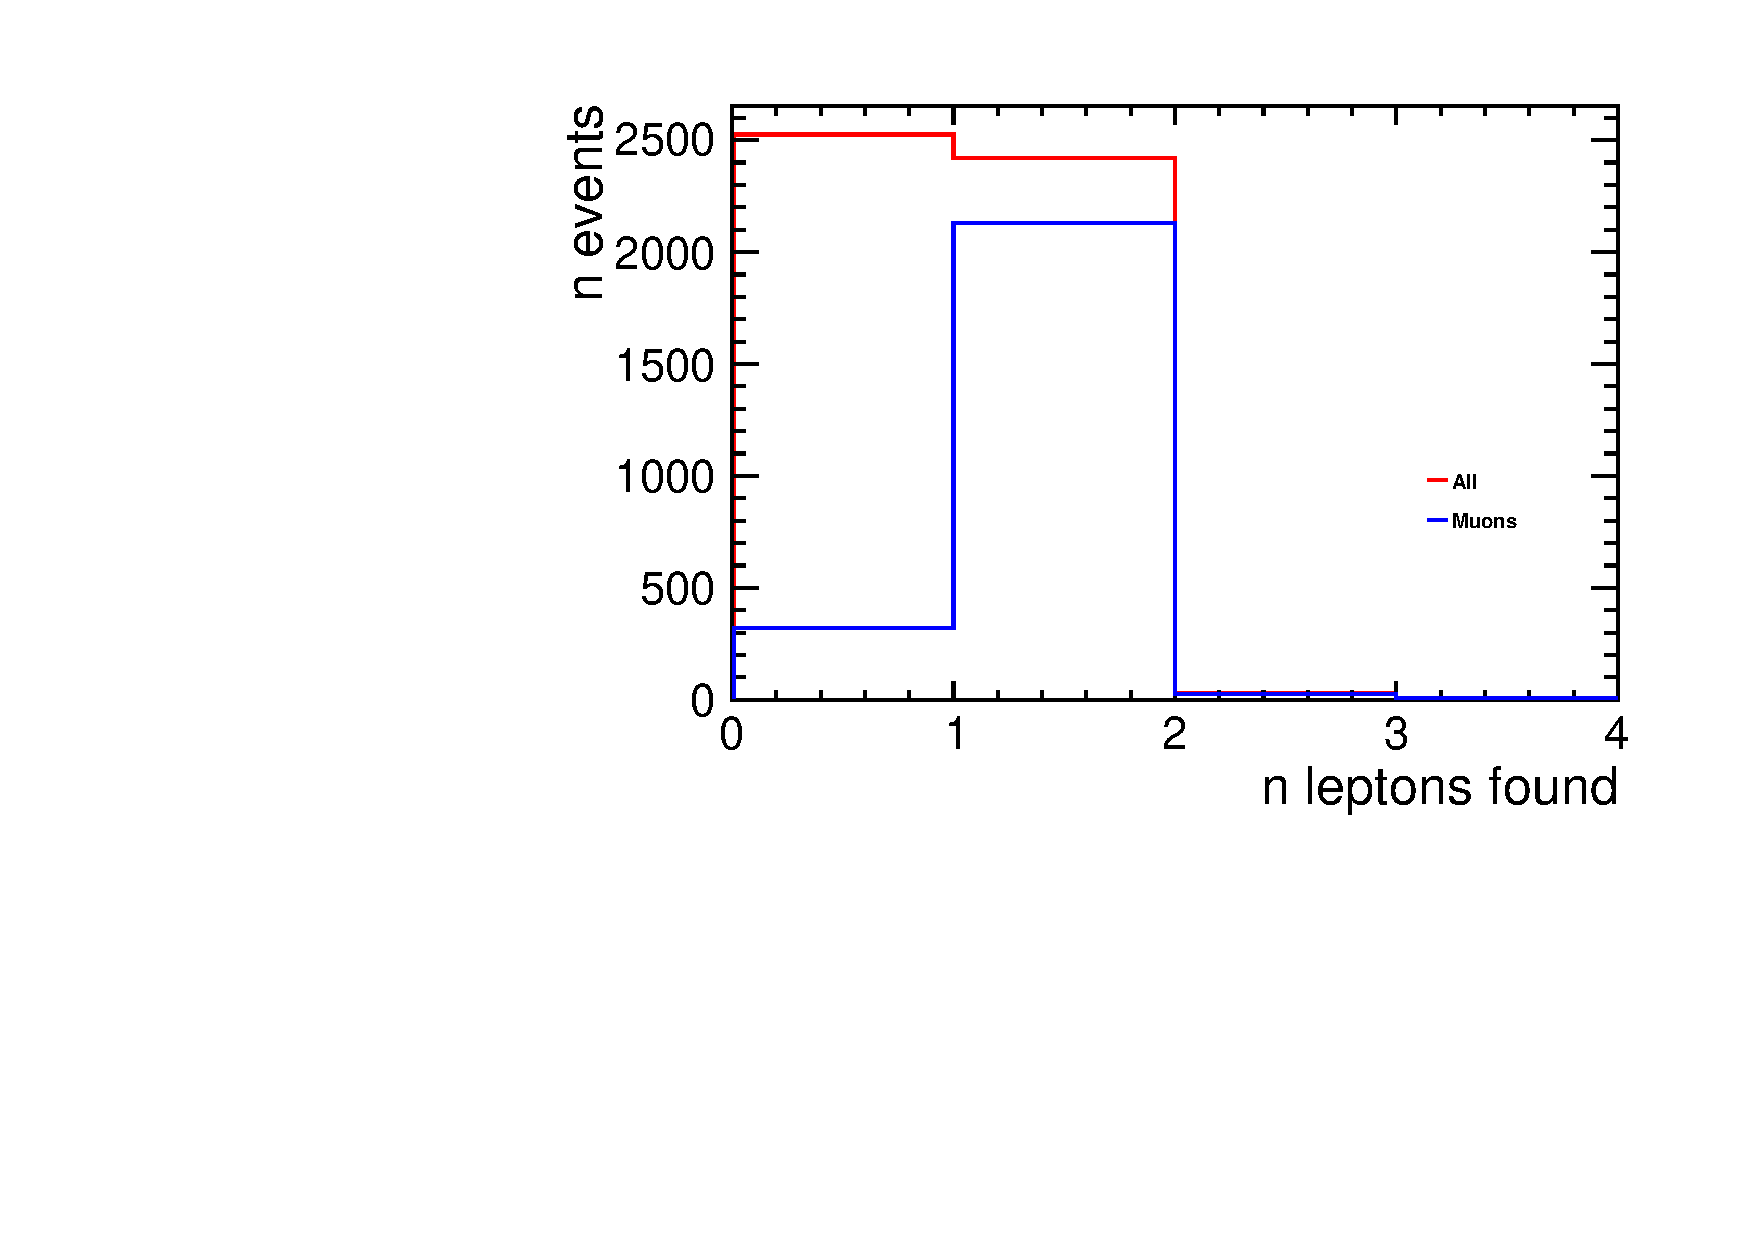
\includegraphics[width=0.9\textwidth]{\imagepath/IsolepsFound.pdf}

\end{frame}

% ----------------------------------------------------------------------------

\begin{frame}\frametitle{Back Up Slides \OrangeBF{Logarithmic mass plots}}

    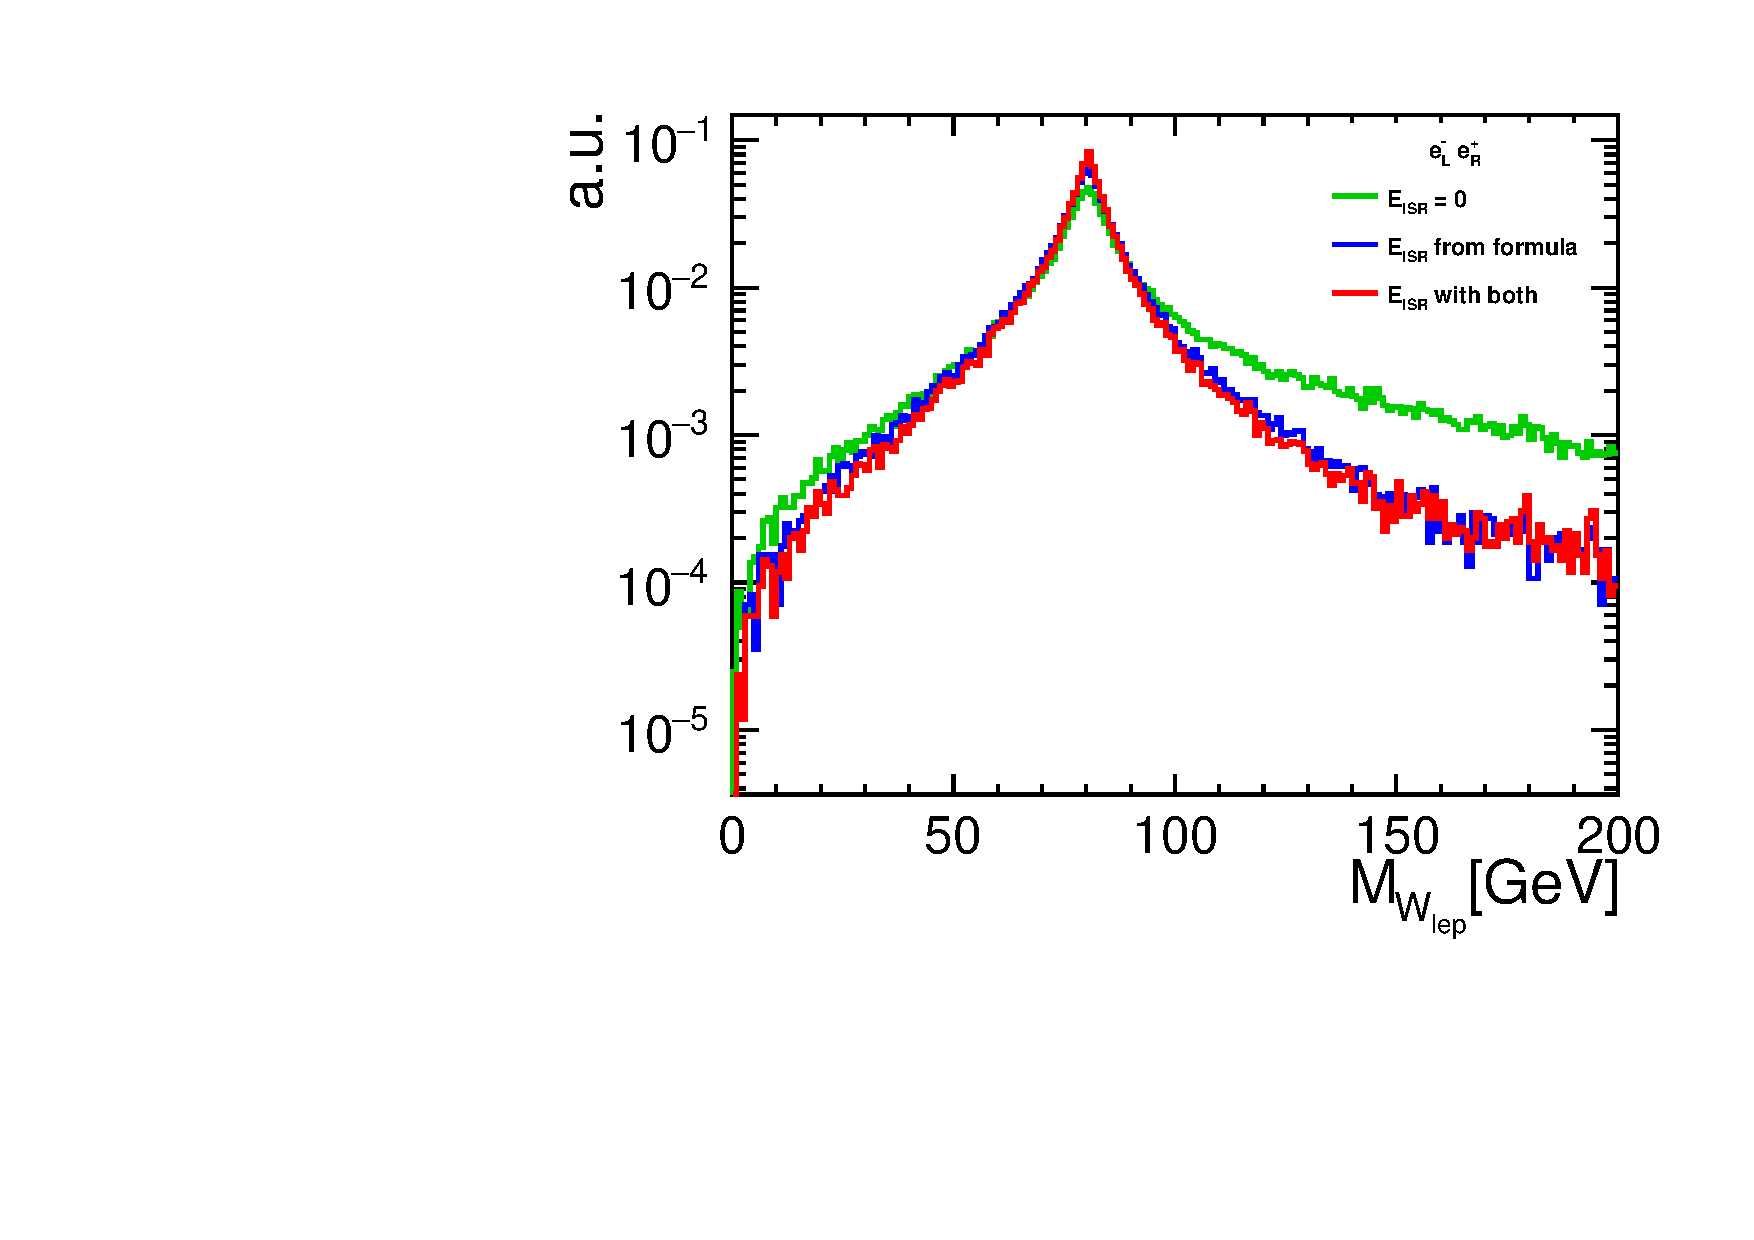
\includegraphics[width=0.49\textwidth]{\imagepath/Mass3_log.pdf}
    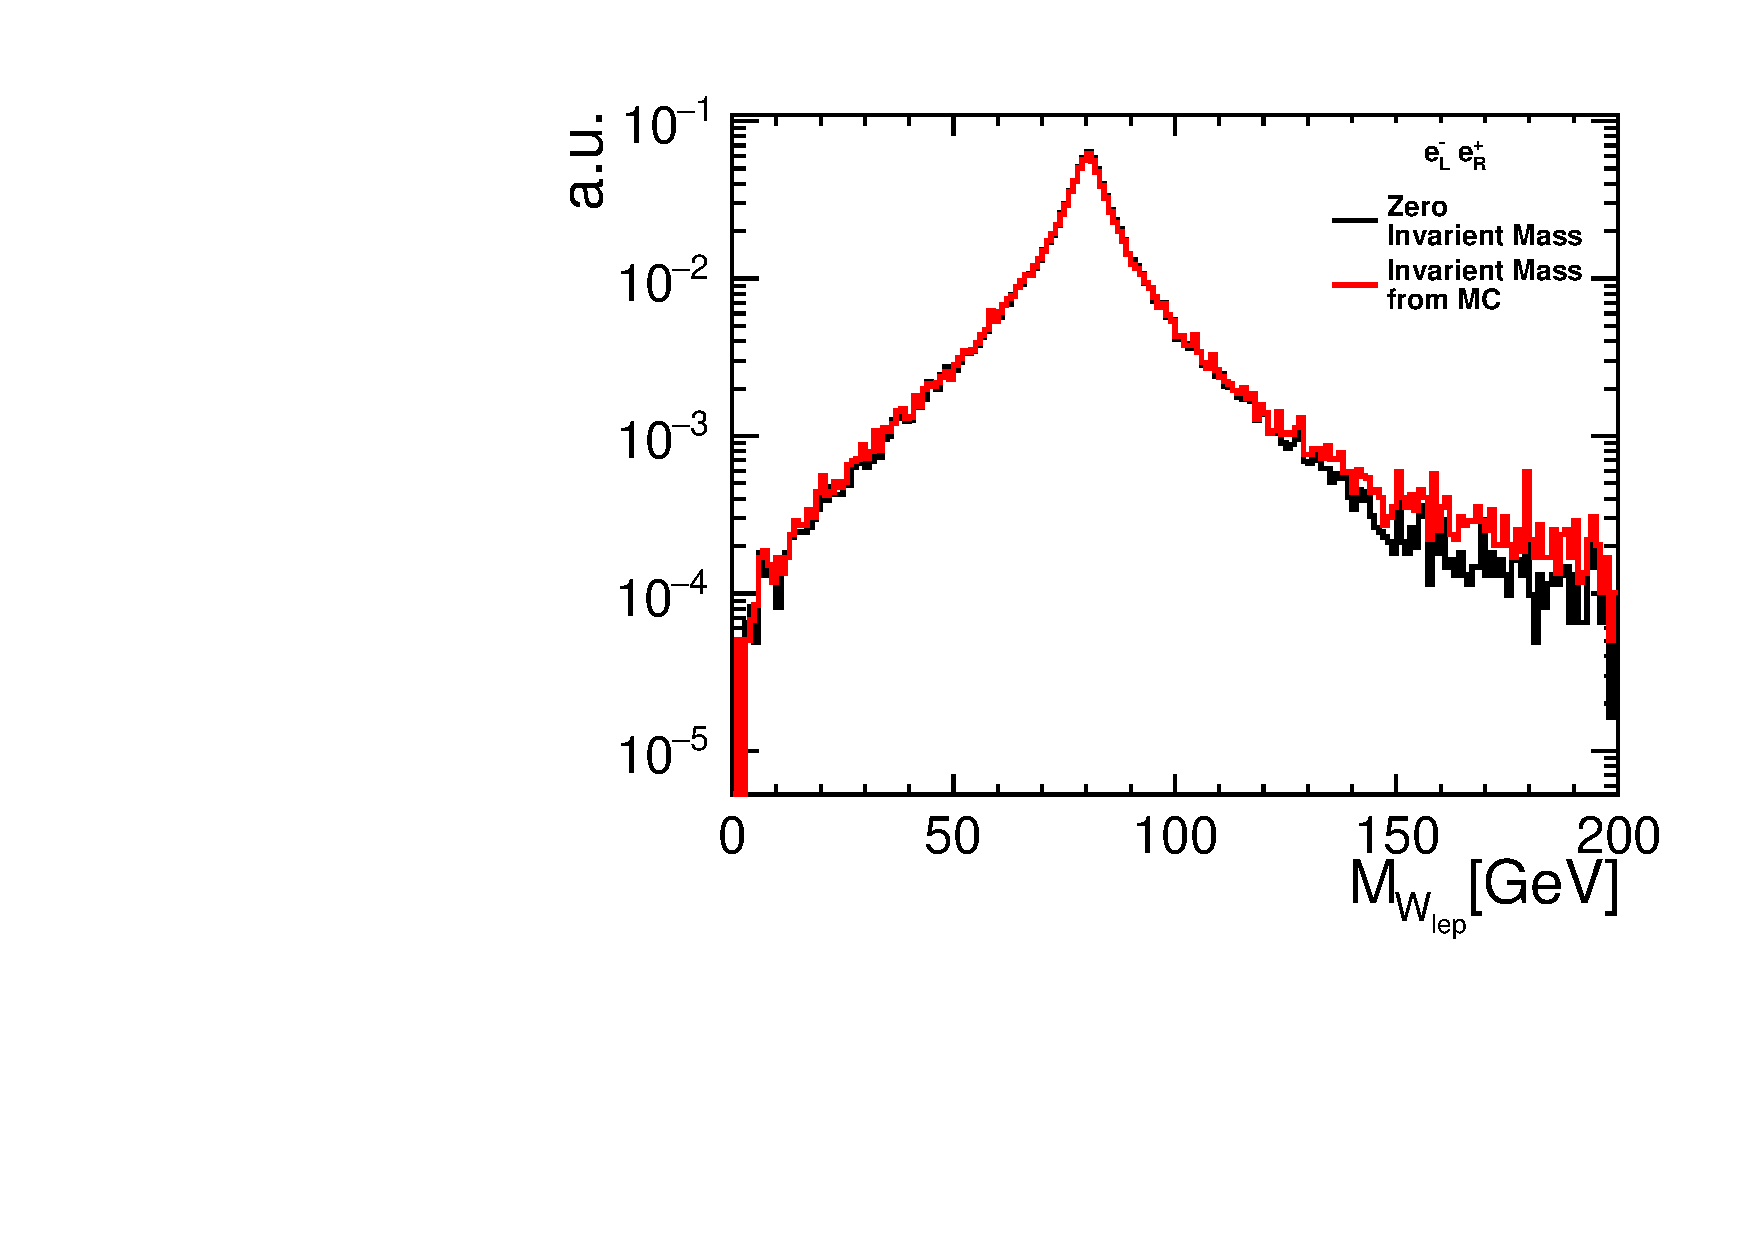
\includegraphics[width=0.49\textwidth]{\imagepath/Mass_log.pdf}

\end{frame}

% ----------------------------------------------------------------------------

\begin{frame}\frametitle{Back Up Slides \OrangeBF{MC ISR invariant mass}}

    \begin{minipage}{0.49\textwidth}
        \centering
        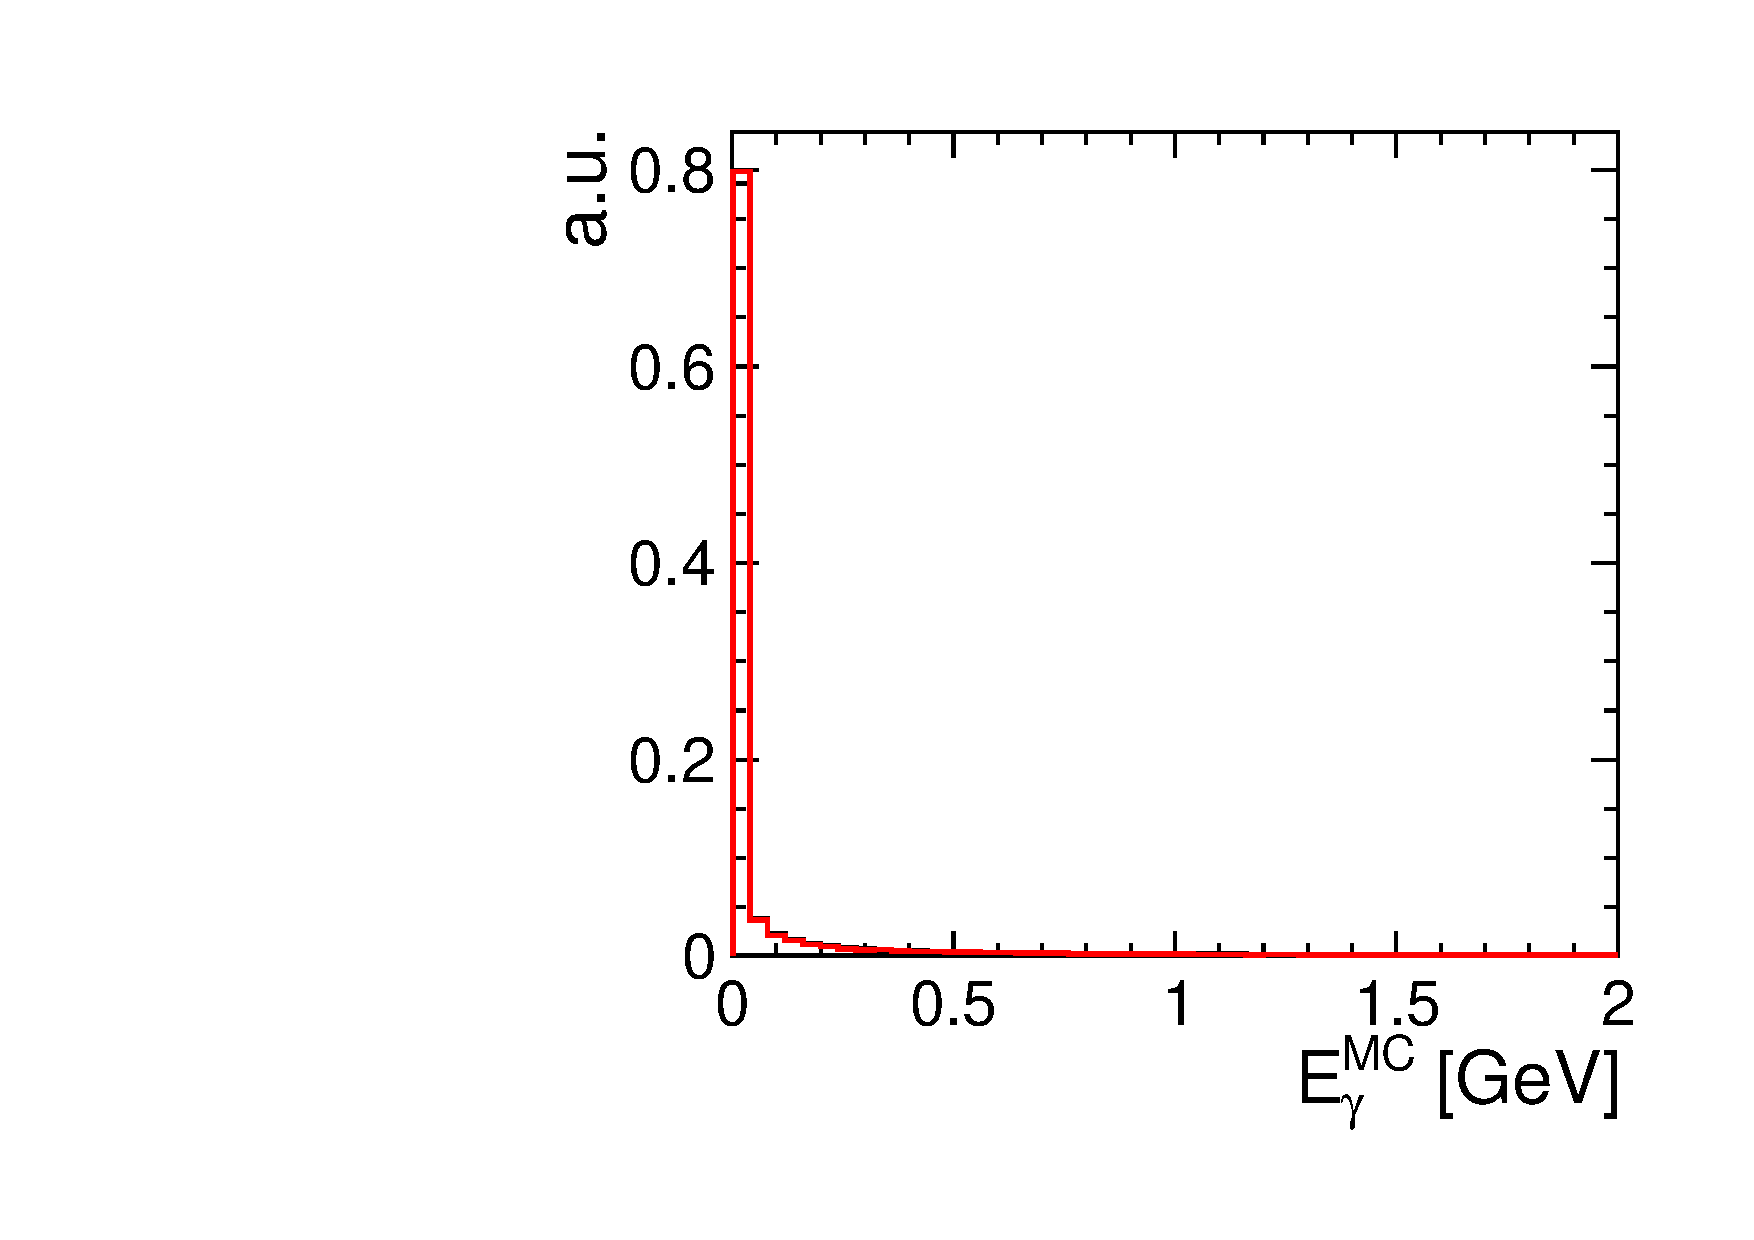
\includegraphics[width=\textwidth]{\imagepath/MCPhotonMass.pdf}
    \end{minipage}
    \begin{minipage}{0.49\textwidth}
        \centering
        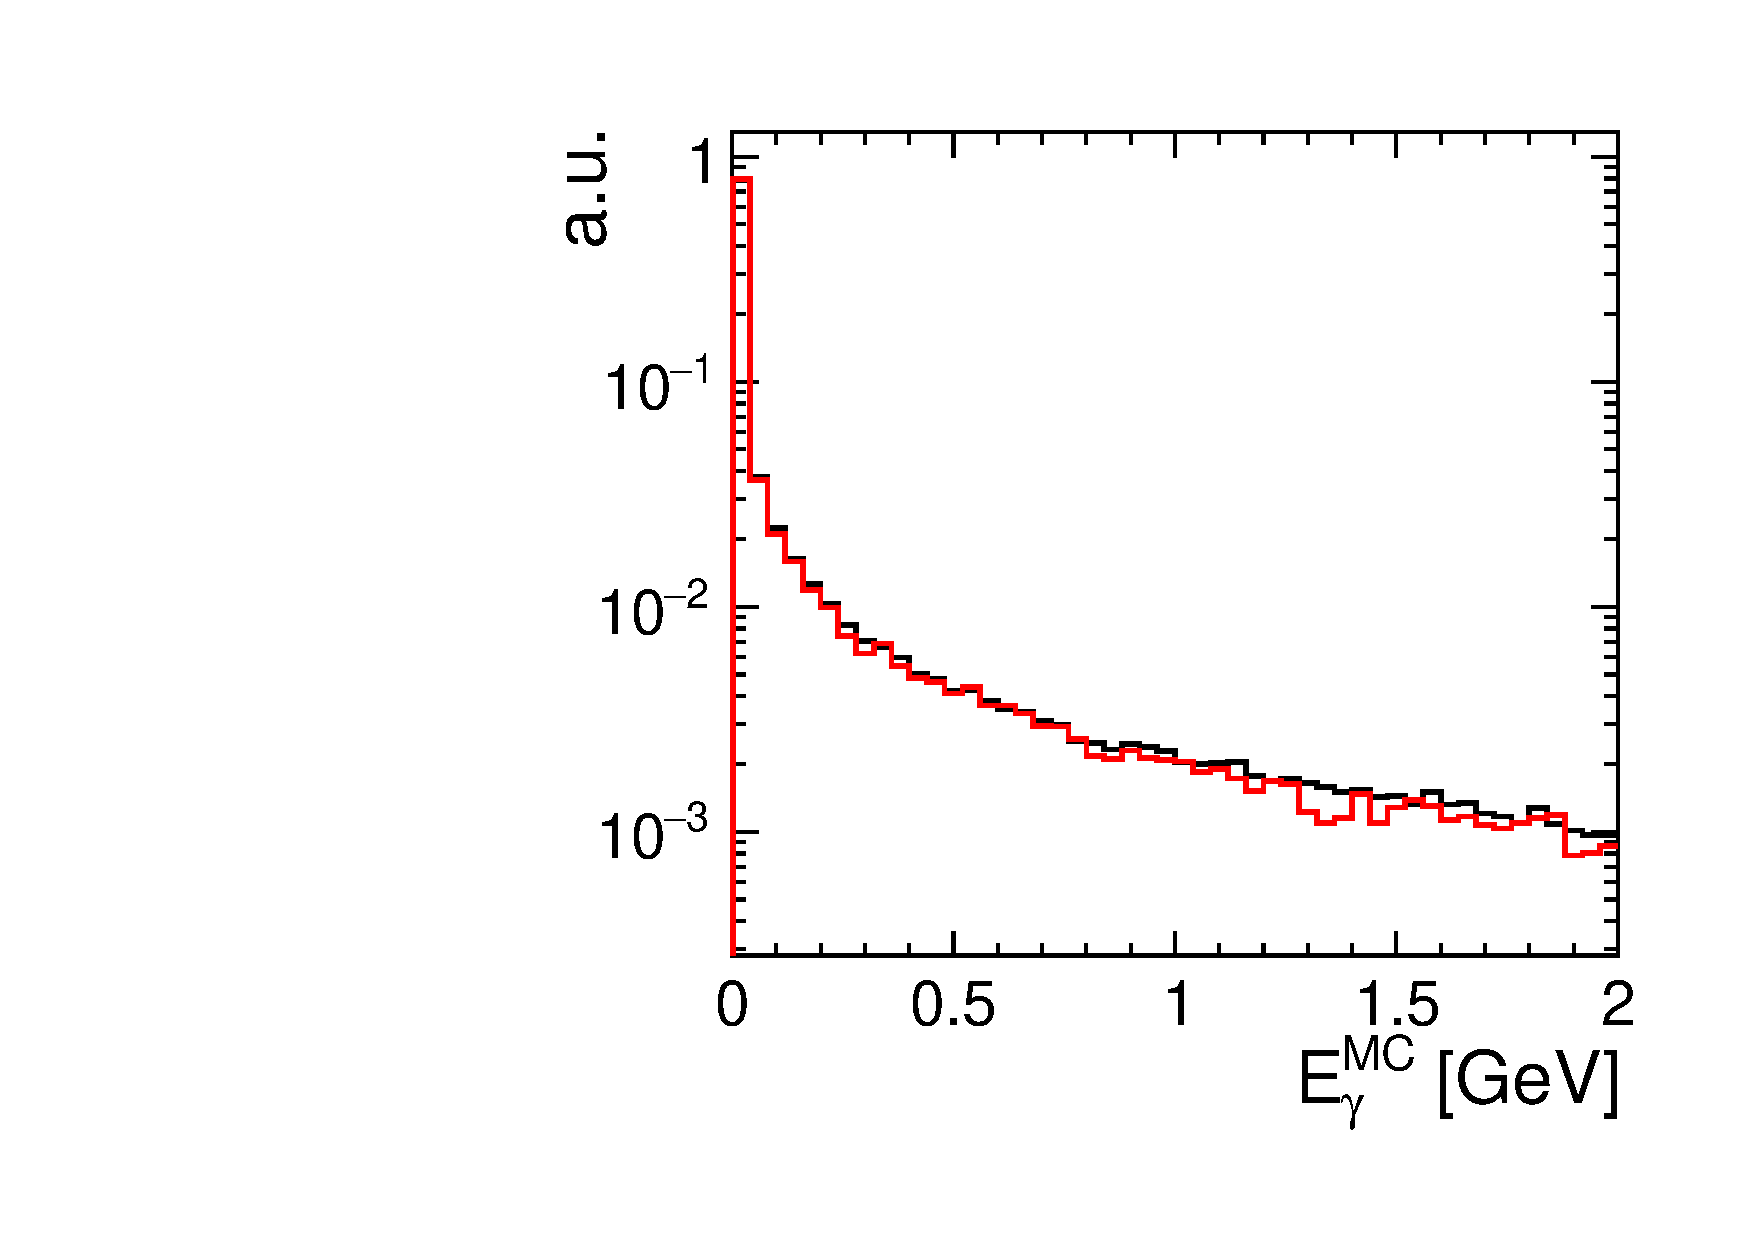
\includegraphics[width=\textwidth]{\imagepath/MCPhotonMass_log.pdf}
    \end{minipage}
\end{frame}

% ----------------------------------------------------------------------------

\begin{frame}\frametitle{Back Up Slides \OrangeBF{Negative Energy}}

    \begin{minipage}{0.49\textwidth}
        \begin{equation*}
          {E}_{\gamma} = \frac{ {(500 - E)}^2 - {p}^{2}}{1000 -2 E  \mp 2{p}_{z}}
        \end{equation*}
        \begin{itemize}
        \item ${E}_{\gamma} < 0$ in \sim 20\% of events
        \item $m_{inv}^{2} < 0$
        \end{itemize}
    \end{minipage}\hfill
    \begin{minipage}{0.49\textwidth}
        \resizebox{0.95\linewidth}{!}{%
        \centering
        \begin{tikzpicture}
  \begin{feynman}[scale=1] % using the vertex in brackets () allows fixing of vertex
    \vertex (m) at (-1, 0);
    \vertex (n) at (0.5, 0);

    \vertex (r) at (-1.7,-0.5);
    \vertex (s) at (-1.7, 0.5);

    \vertex (a) at (-1.5,-1);s
    \vertex (b) at ( 1.75,-1) ;
    \vertex (c) at (-1.5, 1);
    \vertex (d) at ( 1.75, 1) ;

    \vertex (u) at ( 3.5,-1.5) {$l^-$};
    \vertex (v) at ( 3.5,-0.5) {$\bar{\nu}_l$};

    \vertex (q1) at ( 3.5, 1.5) {$q$};
    \vertex (q2) at ( 3.5, 0.5) {$\bar{q'}$};

    \vertex (i1) at (-3,-1) {$e^-$};
    \vertex (i2) at (-3, 1) {$e^+$};

    \vertex (p1) at (0,-1.5) {$\gamma$};
    \vertex (p2) at (0, 1.5) {$\gamma$};

    \diagram* {
      (i1) -- [fermion] (r) --[fermion] (m) ,
      (i2) -- [anti fermion] (s) -- [anti fermion] (m) ,
      (m) -- [photon, edge label=$Z/\gamma$] (n),
      (b) -- [photon, edge label=$W^-$, swap] (n),
      (d) -- [photon, edge label=$W^+$] (n),
      (b) -- [fermion] (u),
      (b) -- [anti fermion] (v),
      (d) -- [fermion] (q1),
      (d) -- [anti fermion] (q2),
      (r) -- [photon] (p1),
      (s) -- [photon] (p2),
    };
  \end{feynman}
\end{tikzpicture}

        }
        \\
        \centering
        \begin{tikzpicture}
  \begin{feynman}[scale=1] % using the vertex in brackets () allows fixing of vertex
    \vertex (n) at (0, 0.75) ;
    \vertex (m) at (0, -0.75) ;

    \vertex (r) at (-1.2,-1);
    \vertex (s) at (-1.2, 1);

    \vertex (a) at (-1,-1) ;
    \vertex (b) at ( 1.25,-1) ;
    \vertex (c) at (-1, 1);
    \vertex (d) at ( 1.25, 1) ;

    \vertex (u) at ( 3,-1.5) {$l^-$};
    \vertex (v) at ( 3,-0.5) {$\bar{\nu}_l$};

    \vertex (q1) at ( 3, 1.5) {$q$};
    \vertex (q2) at ( 3, 0.5) {$\bar{q'}$};

    \vertex (i1) at (-2.5,-1) {$e_L^-$};
    \vertex (i2) at (-2.5, 1) {$e_R^+$};

    \vertex (p1) at (0,-1.5) {$\gamma$};
    \vertex (p2) at (0, 1.5) {$\gamma$};


    \diagram* {
      (i1) -- [fermion] (r) --[fermion] (m) -- [fermion, edge label=$\nu_e$] (n),
      (i2) -- [anti fermion] (s) -- [anti fermion] (n),
      (b) -- [photon, edge label=$W^-$, swap] (m),
      (d) -- [photon, edge label=$W^+$] (n),
      (b) -- [fermion] (u),
      (b) -- [anti fermion] (v),
      (d) -- [fermion] (q1),
      (d) -- [anti fermion] (q2),
      (r) -- [photon] (p1),
      (s) -- [photon] (p2),

    };
  \end{feynman}
\end{tikzpicture}

    \end{minipage}

\end{frame}
% ----------------------------------------------------------------------------

\begin{frame}\frametitle{Back Up Slides \OrangeBF{Lortenz boost}}

     \begin{minipage}{0.49\textwidth}
         \begin{itemize}
             \item The ${e}^{-}{e}^{+}$ collision is \CyanBF{not in the center of mass frame}
             \begin{equation}
                 {p}^{\mu} = ( 500 \sin{(\frac{0.014}{2})}, 0, 0, 500)\, GeV.
             \end{equation}
        \end{itemize}
     \end{minipage}\hfill
     \begin{minipage}{0.49\textwidth}
         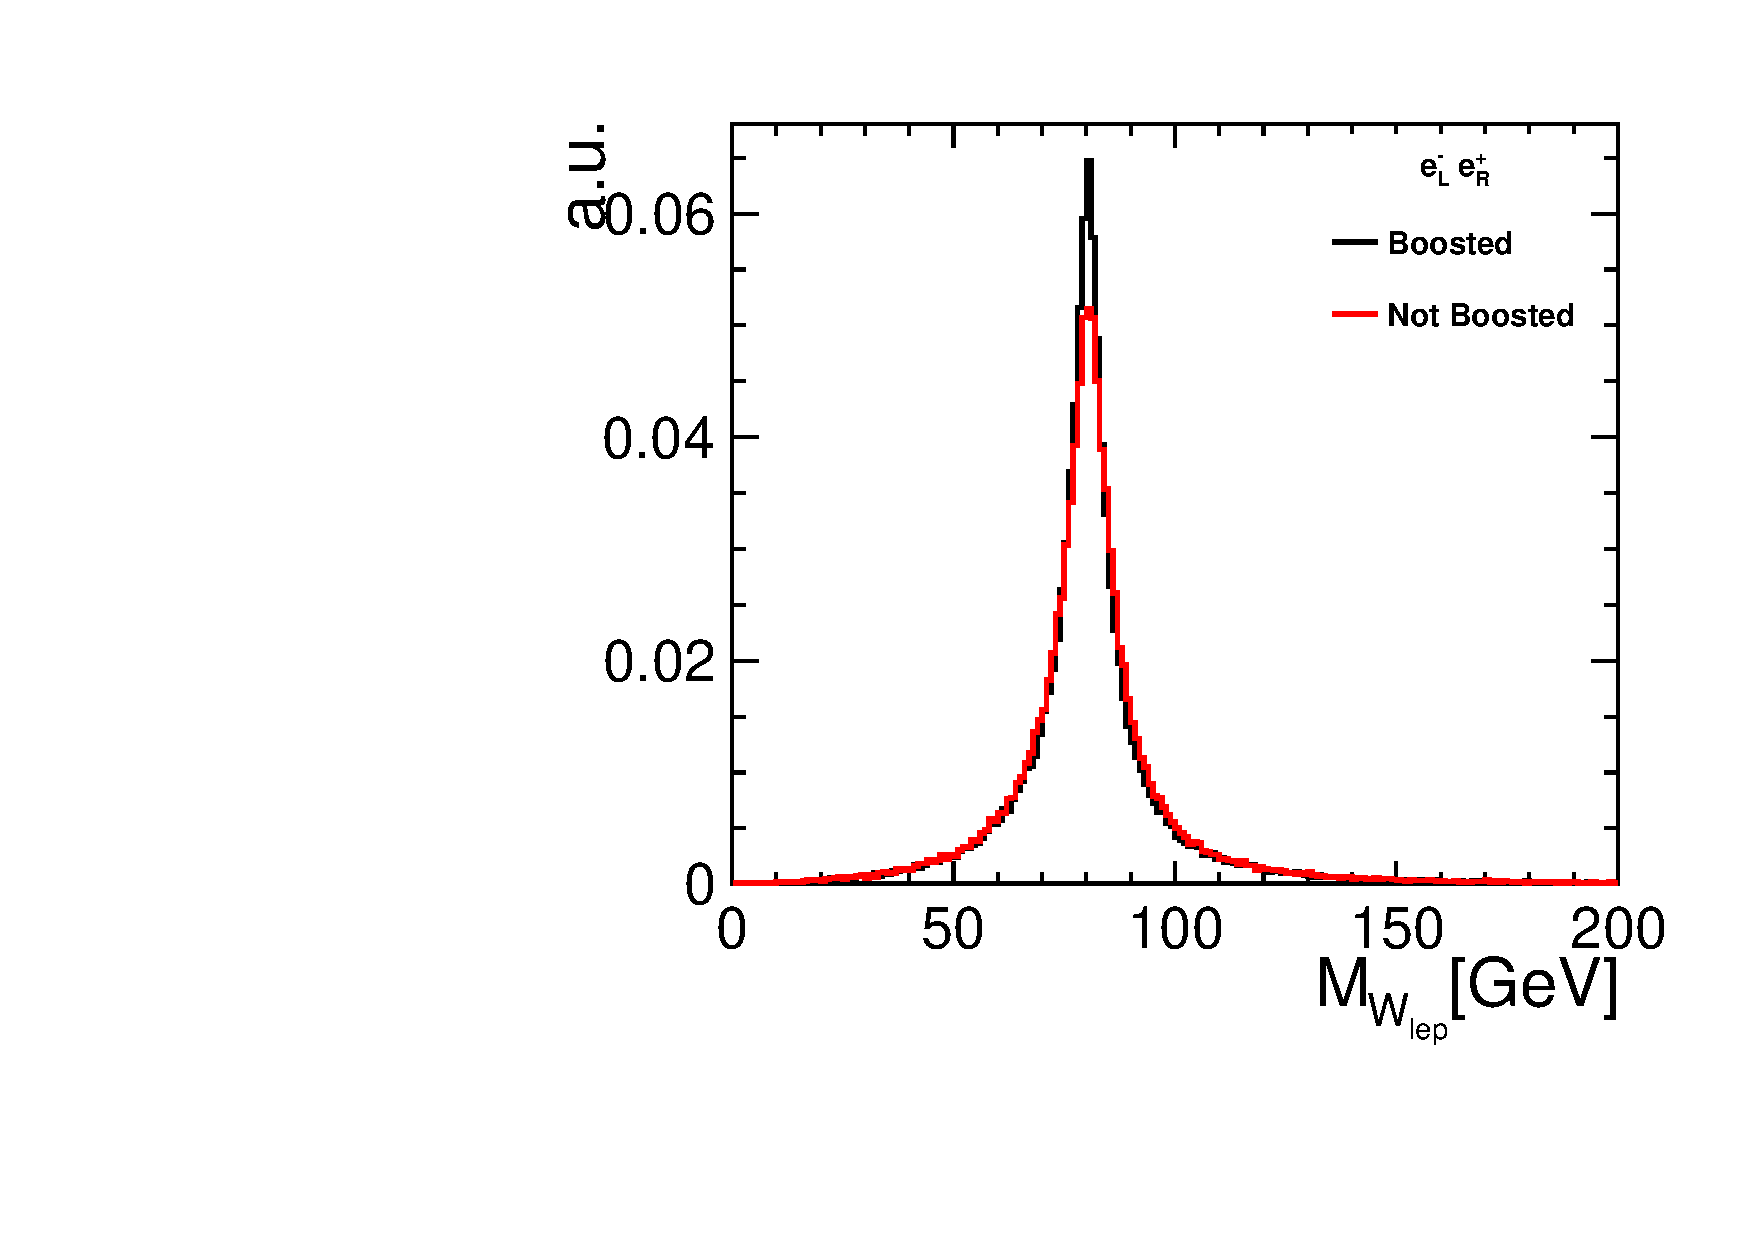
\includegraphics[width=\textwidth]{\imagepath/Boost.pdf}
     \end{minipage}

\end{frame}
% ----------------------------------------------------------------------------

\begin{frame}\frametitle{Back Up Slides \OrangeBF{Beam background cheating}}

    \begin{itemize}
        \item Try \CyanBF{cheat beam background} using TrueJet
    \end{itemize}
    \begin{minipage}{0.49\textwidth}
        \centering
        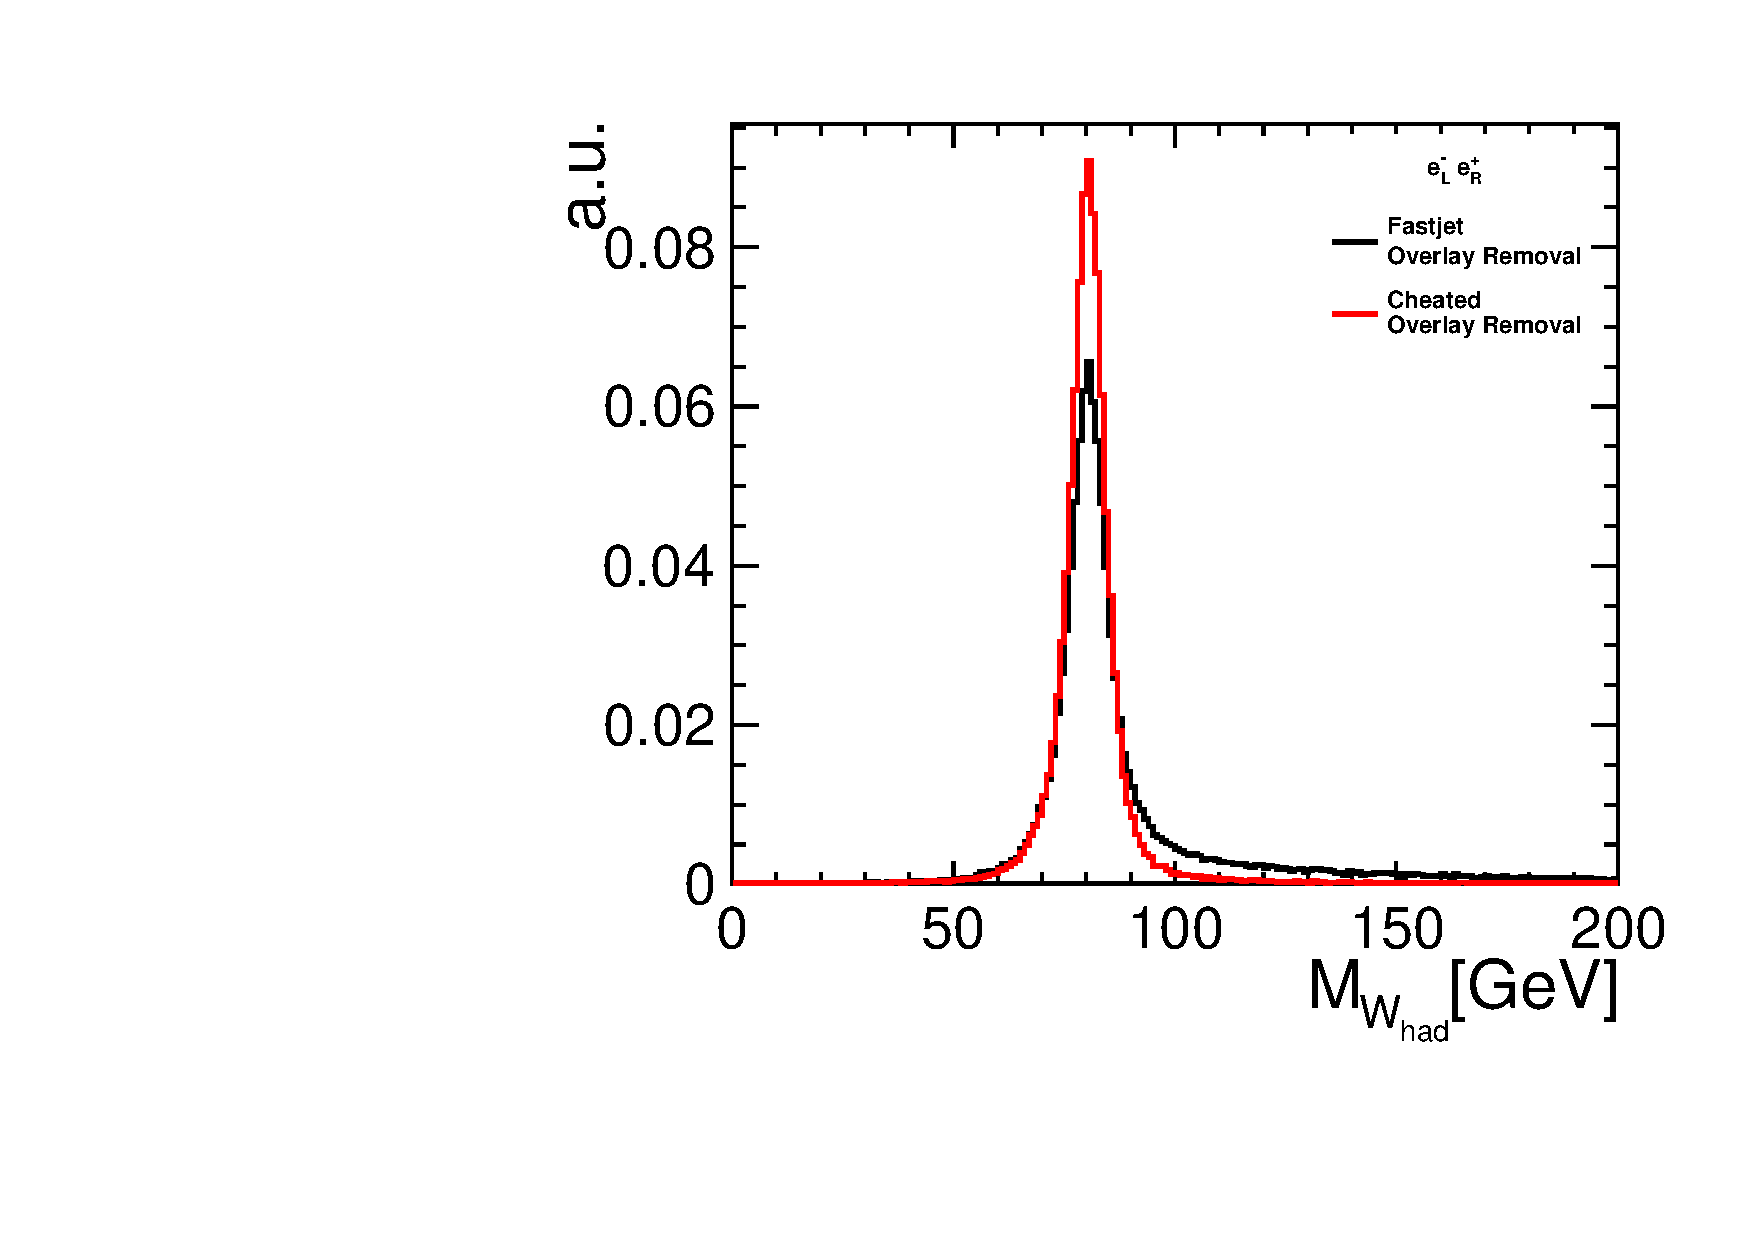
\includegraphics[width=\textwidth]{\imagepath/Jet.pdf}
    \end{minipage}\hfill
    \begin{minipage}{0.49\textwidth}
        \centering
        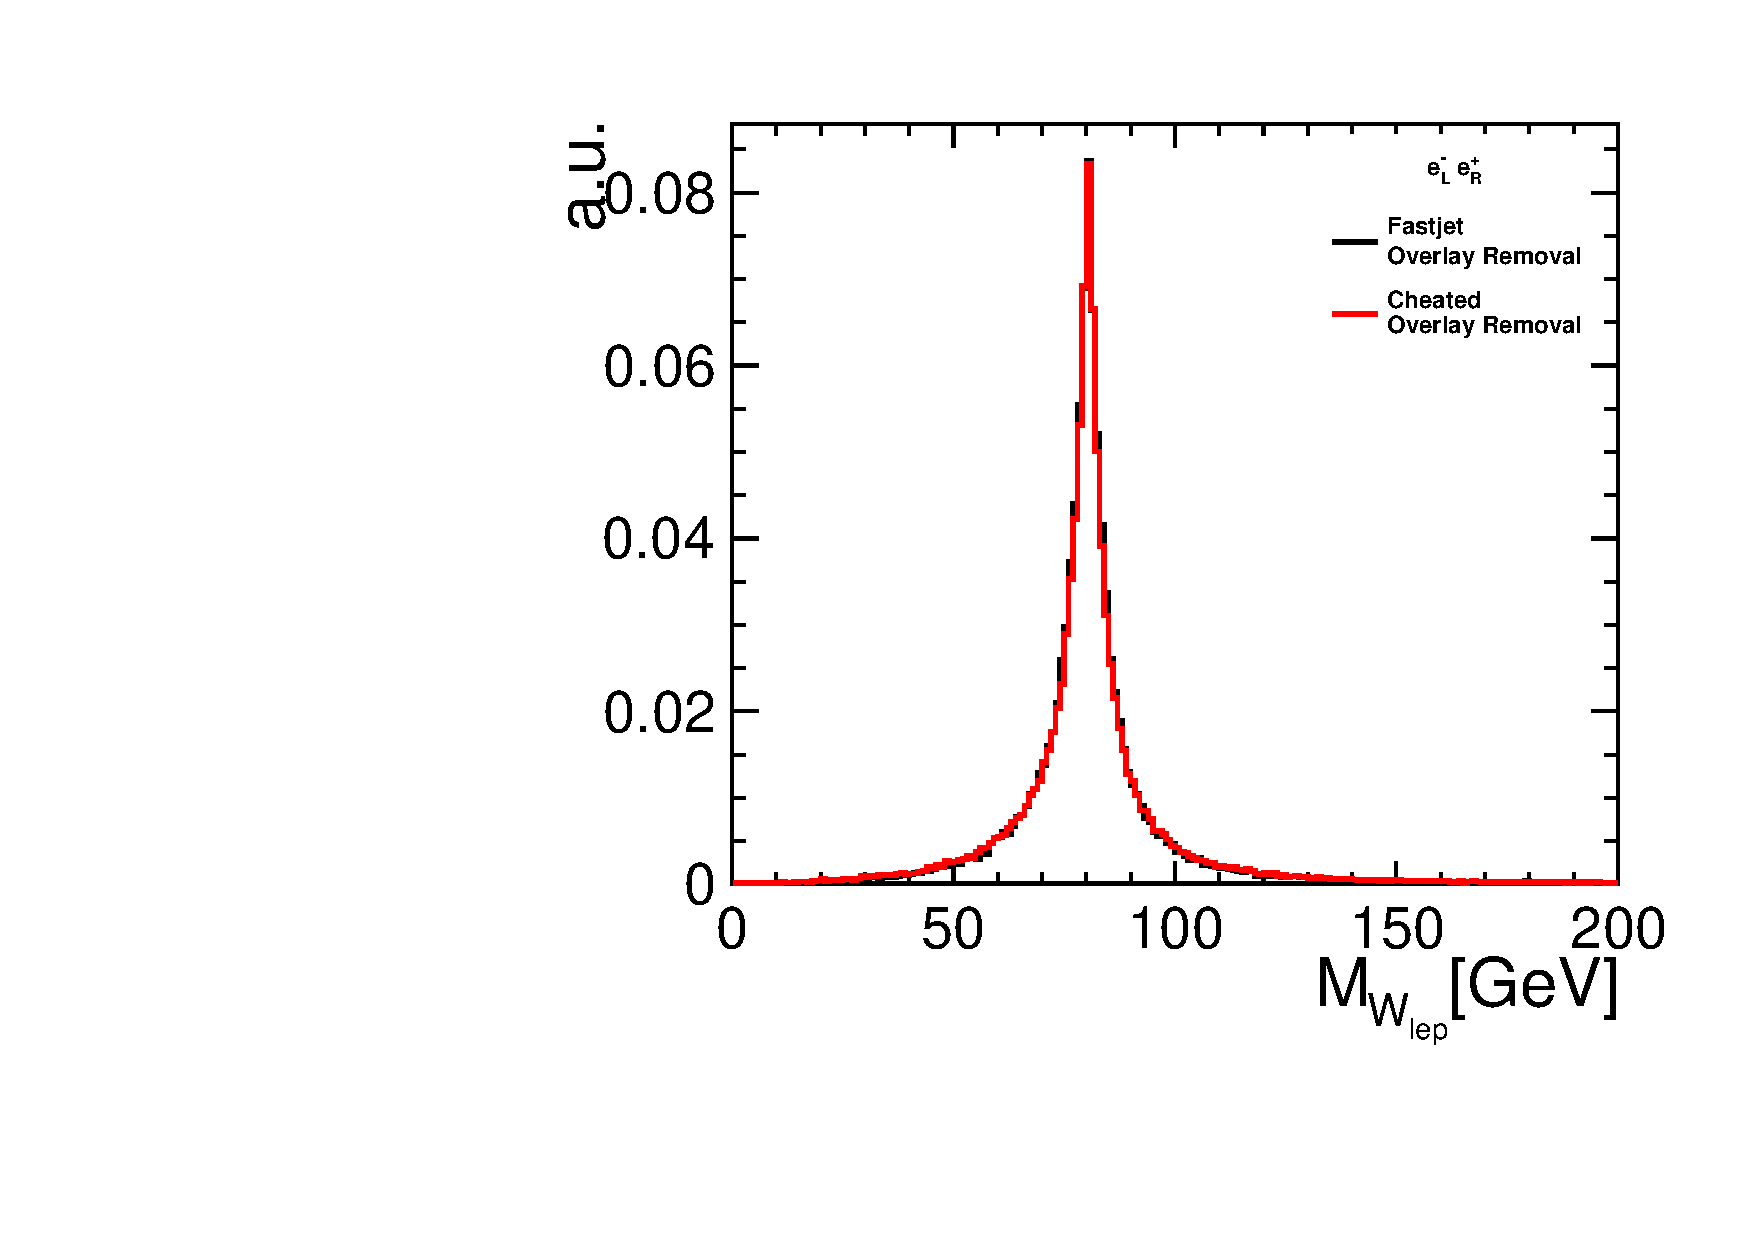
\includegraphics[width=\textwidth]{\imagepath/Lep.pdf}
    \end{minipage}

\end{frame}
% ----------------------------------------------------------------------------

\begin{frame}\frametitle{Back Up Slides \OrangeBF{ISR invarient mass}}

    \begin{itemize}
        \item Invarient mass of the neutrino and ISR photon is nolonger assumed zero.
    \end{itemize}
    \CyanBF{Full energy equation}
    \begin{equation}
        {E}_{\gamma}    = \frac{{\lambda}(500 - E)  \pm {p}_{z}\sqrt{ {\lambda}^{2} - [{(500 - E)}^{2} -{p}_{z}^{2}]{m}_{\gamma}^{2}}}{{(500 - E)}^{2} -   {p}_{z}^{2}}
    \end{equation}
    Where for convenience I have defined \CyanBF{lambda},
    \begin{equation}
        {\lambda} = \frac{1}{2}[{(500 - E)}^2 - {p}^{2} + {m}_{\gamma}^{2} - {m}_{\nu}^{2}] \, .
    \end{equation}

\end{frame}
% ----------------------------------------------------------------------------

\begin{frame}\frametitle{Back Up Slides \OrangeBF{ISR invarient mass}}
    \begin{itemize}
        \item ${m}_{\nu} = 0$ and ${m}_{\gamma}$ from MC
    \end{itemize}
    \centering
    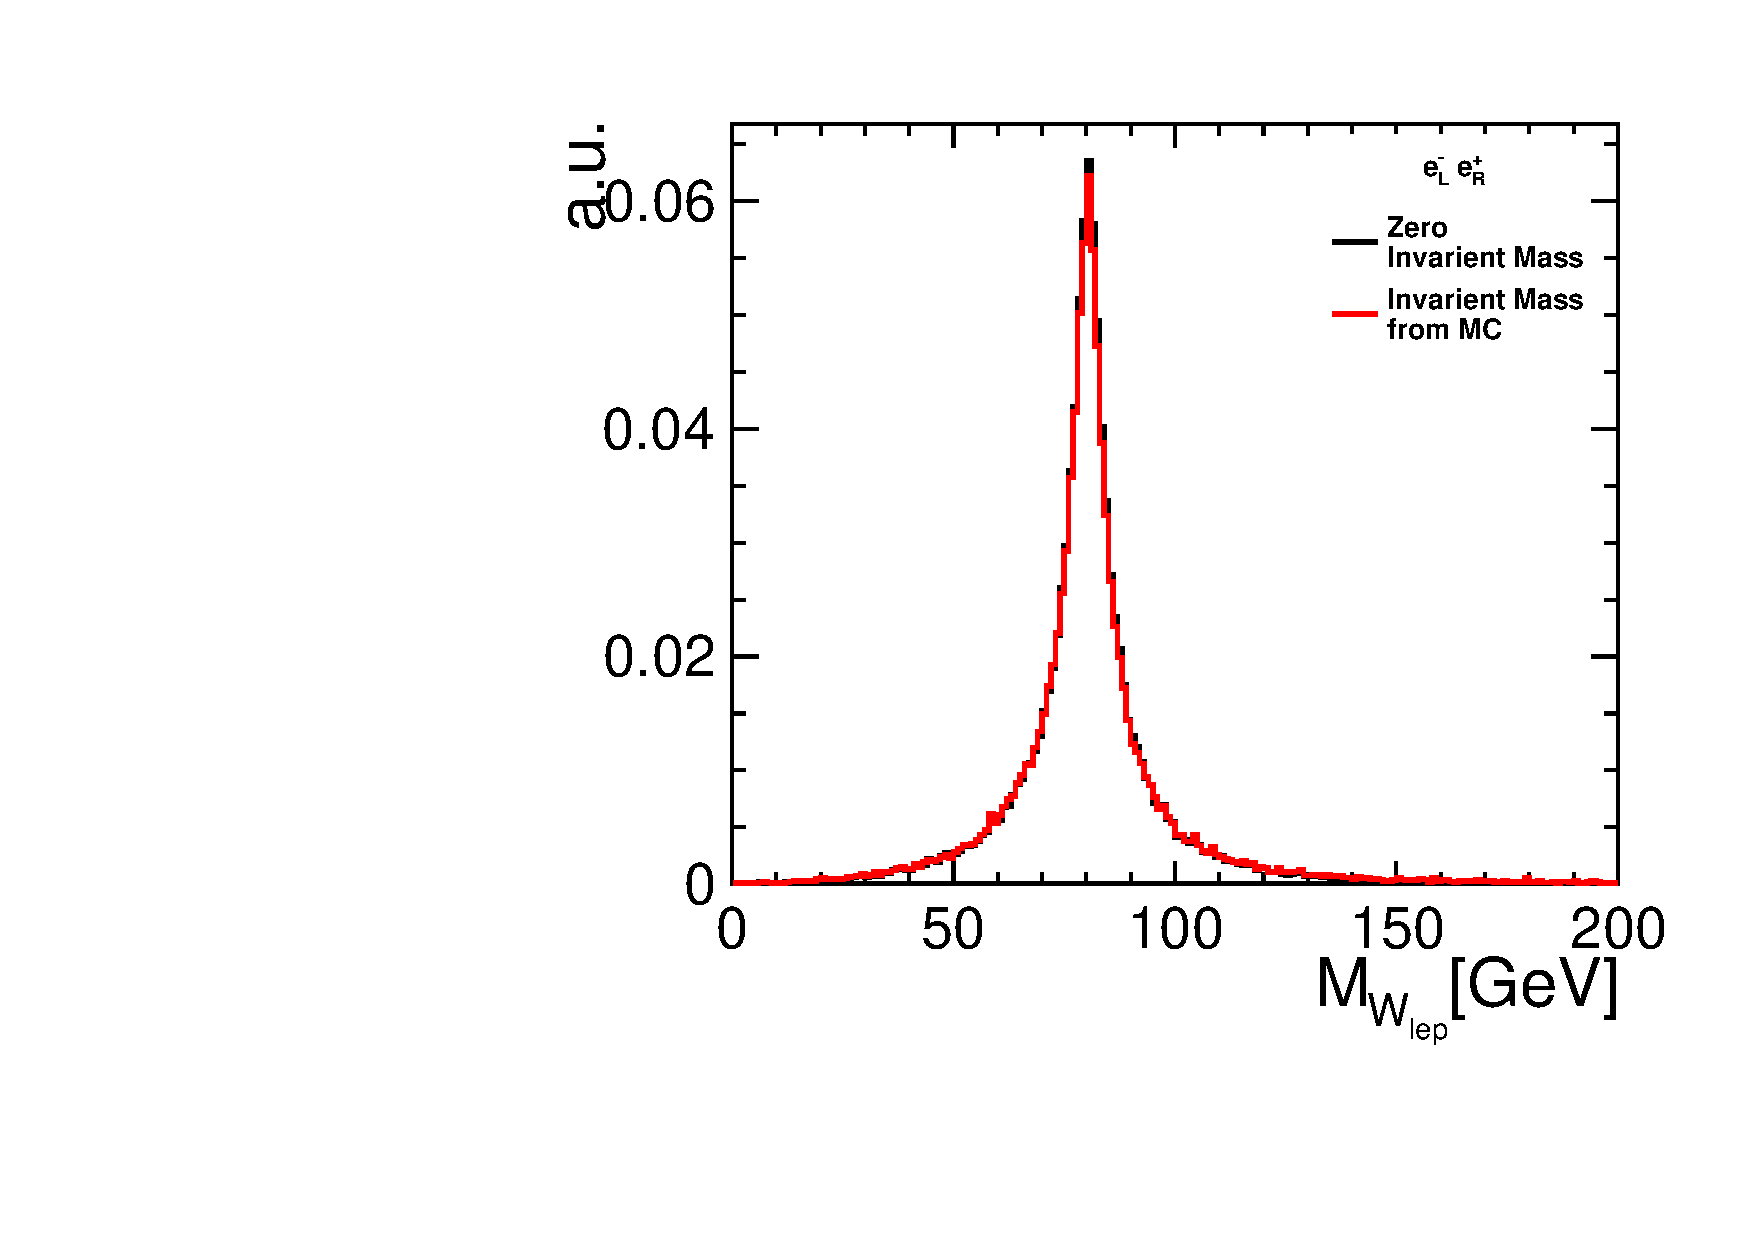
\includegraphics[width=0.6\textwidth]{\imagepath/Mass.pdf}

\end{frame}

% ----------------------------------------------------------------------------

\begin{frame}\frametitle{Back Up Slides \OrangeBF{Cut Flow}}

    \centering
    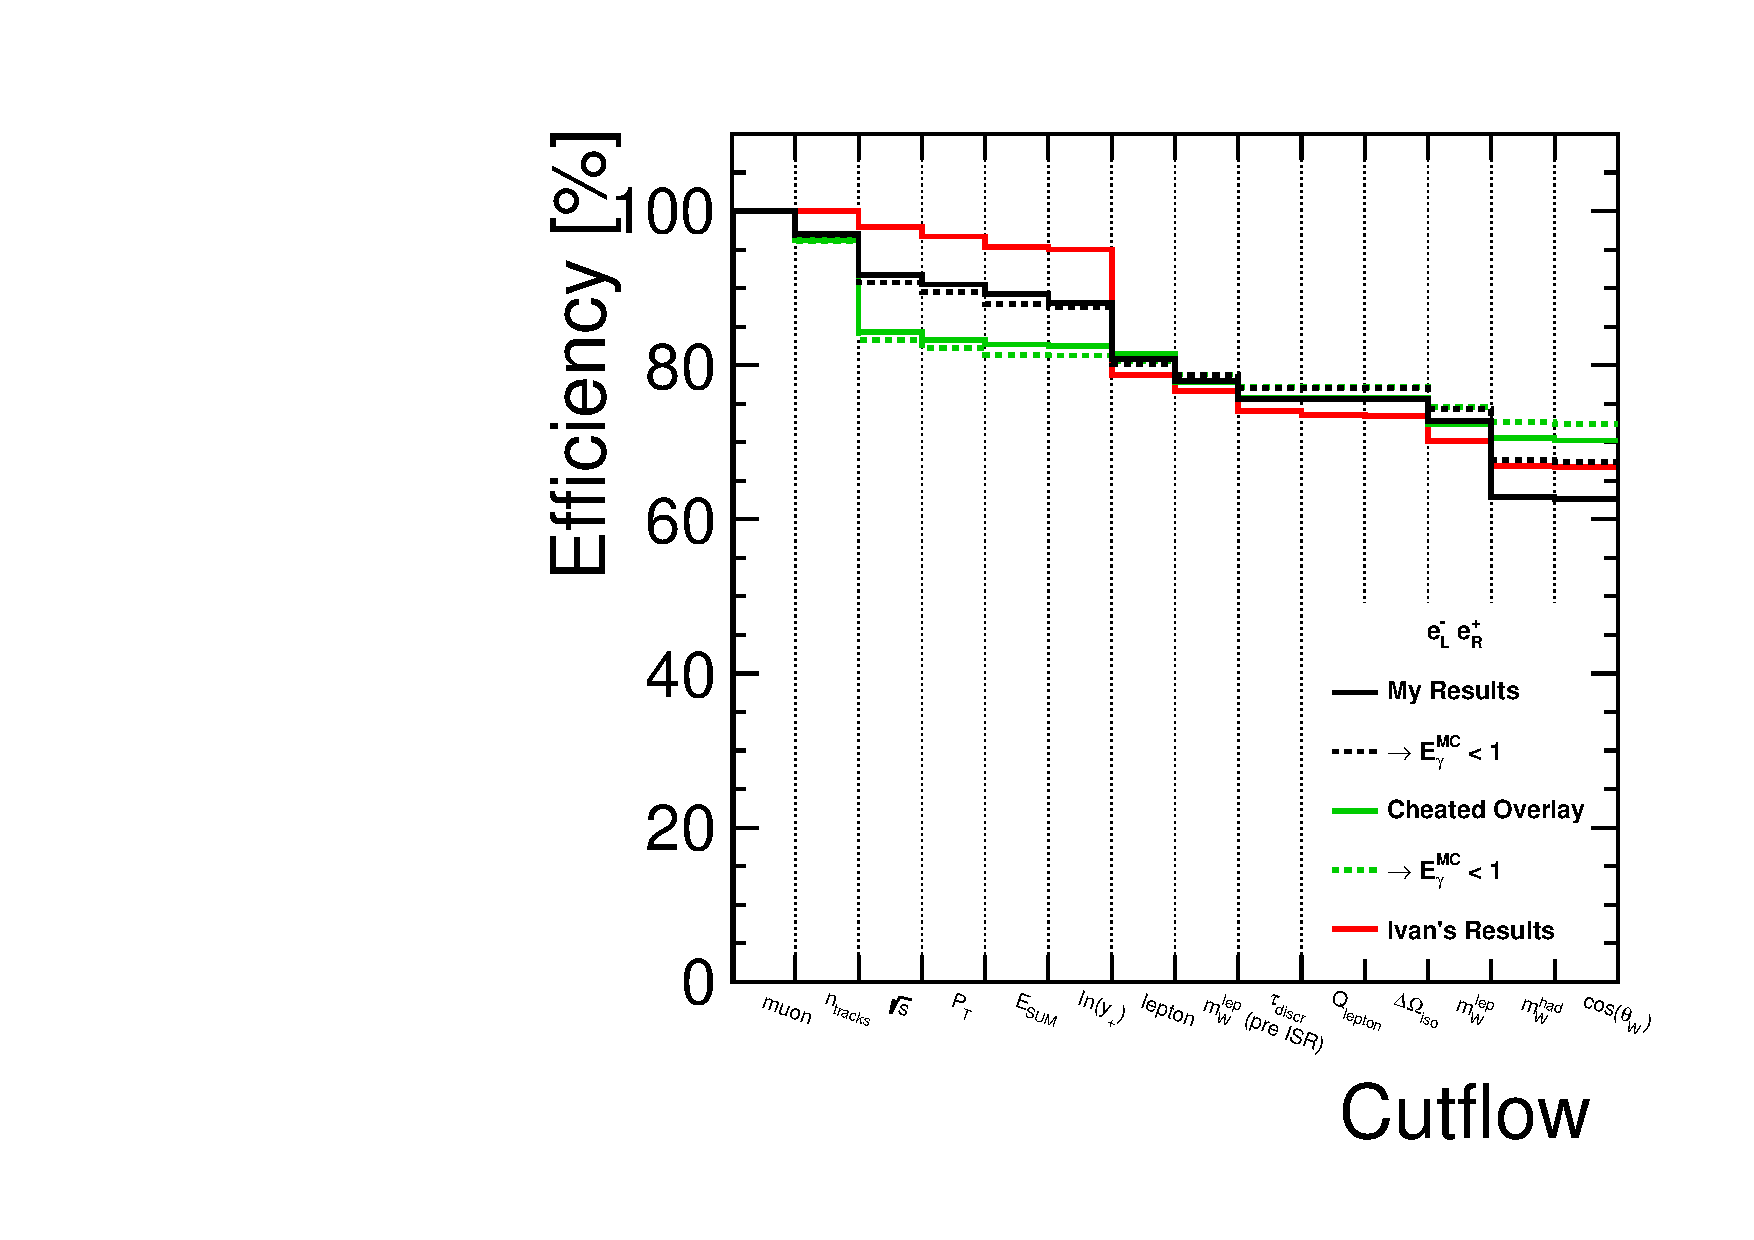
\includegraphics[width=0.6\textwidth]{\imagepath/P_HistFlow3_All.pdf}

\end{frame}

% ----------------------------------------------------------------------------

\begin{frame}\frametitle{Back Up Slides \OrangeBF{New ISR Energy Plots}}

    \begin{minipage}{0.49\textwidth}
        \centering
        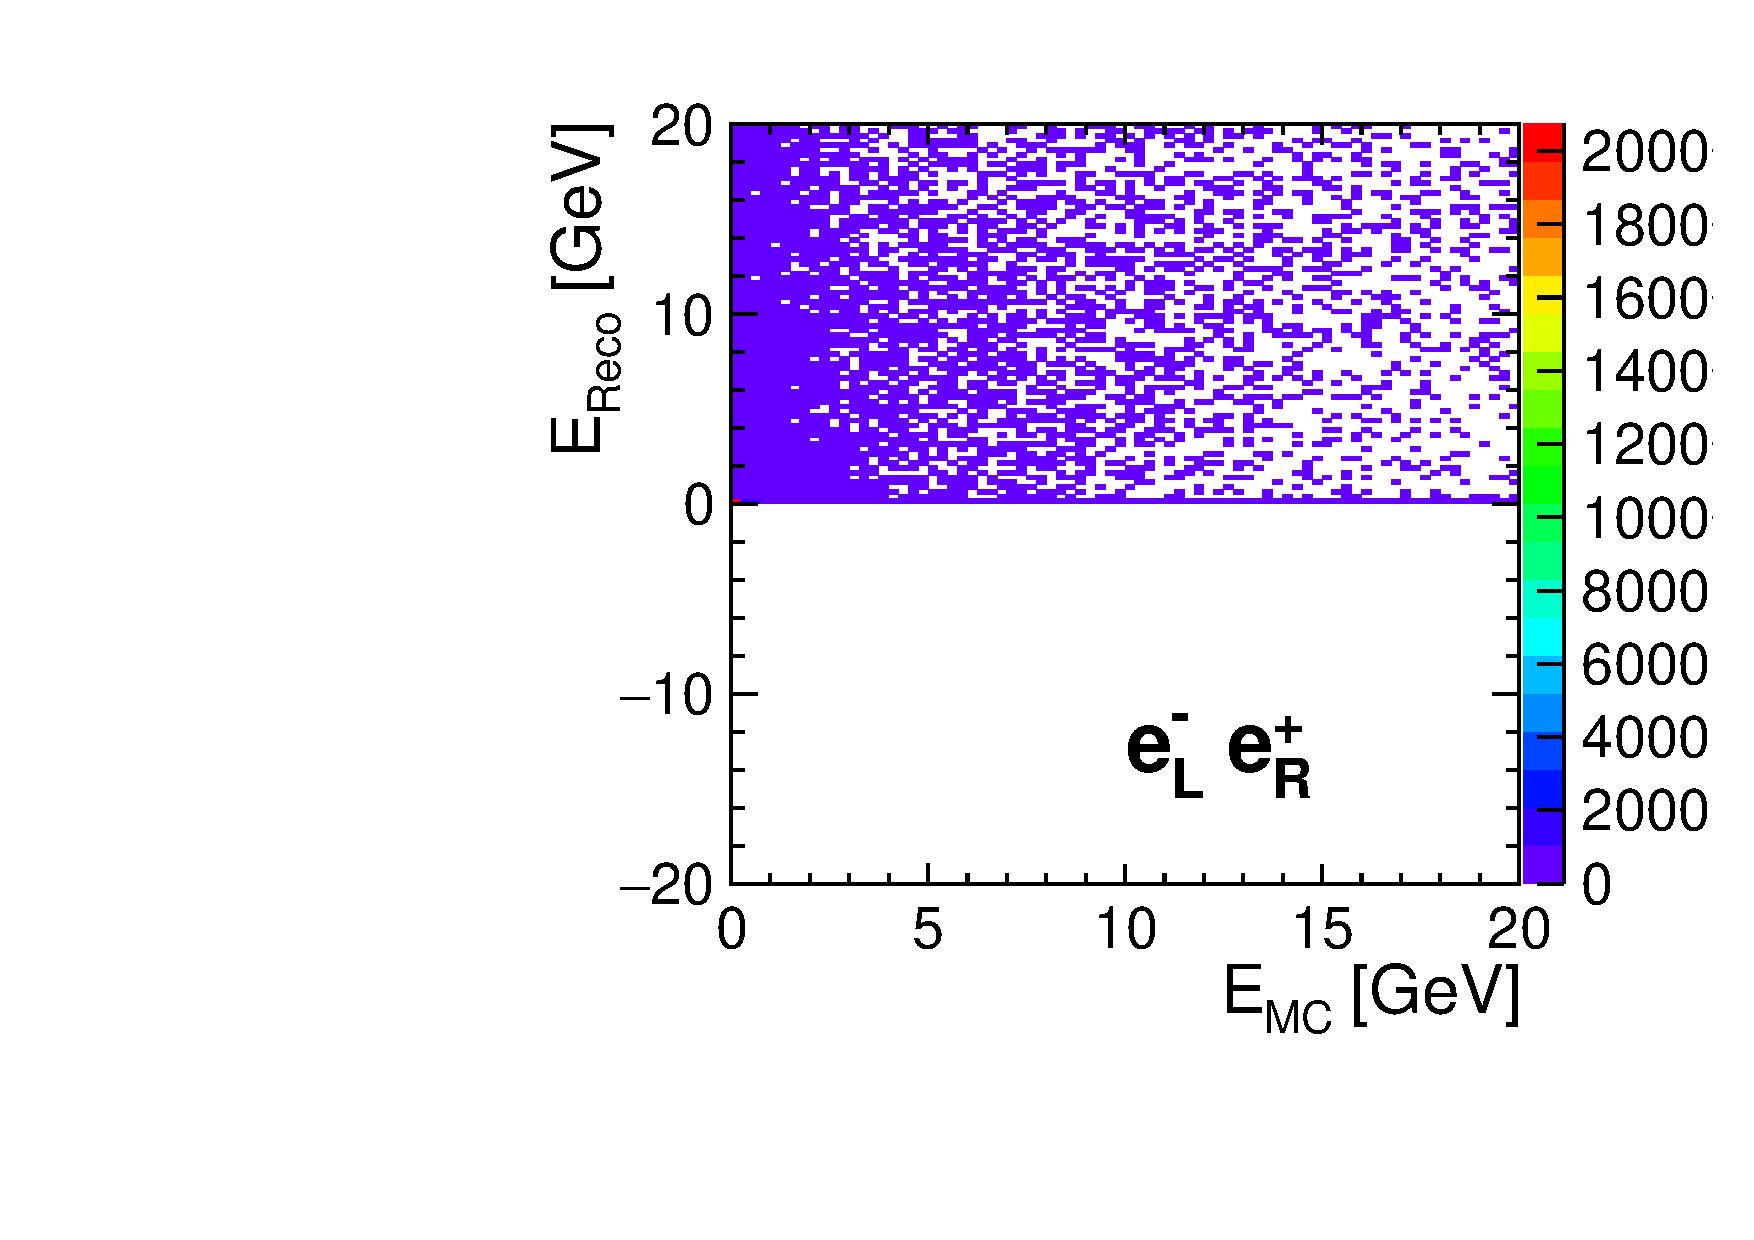
\includegraphics[width=\textwidth]{\imagepath/PhotonEnergy_2D_new.pdf}
    \end{minipage}\hfill
    \begin{minipage}{0.49\textwidth}
        \centering
        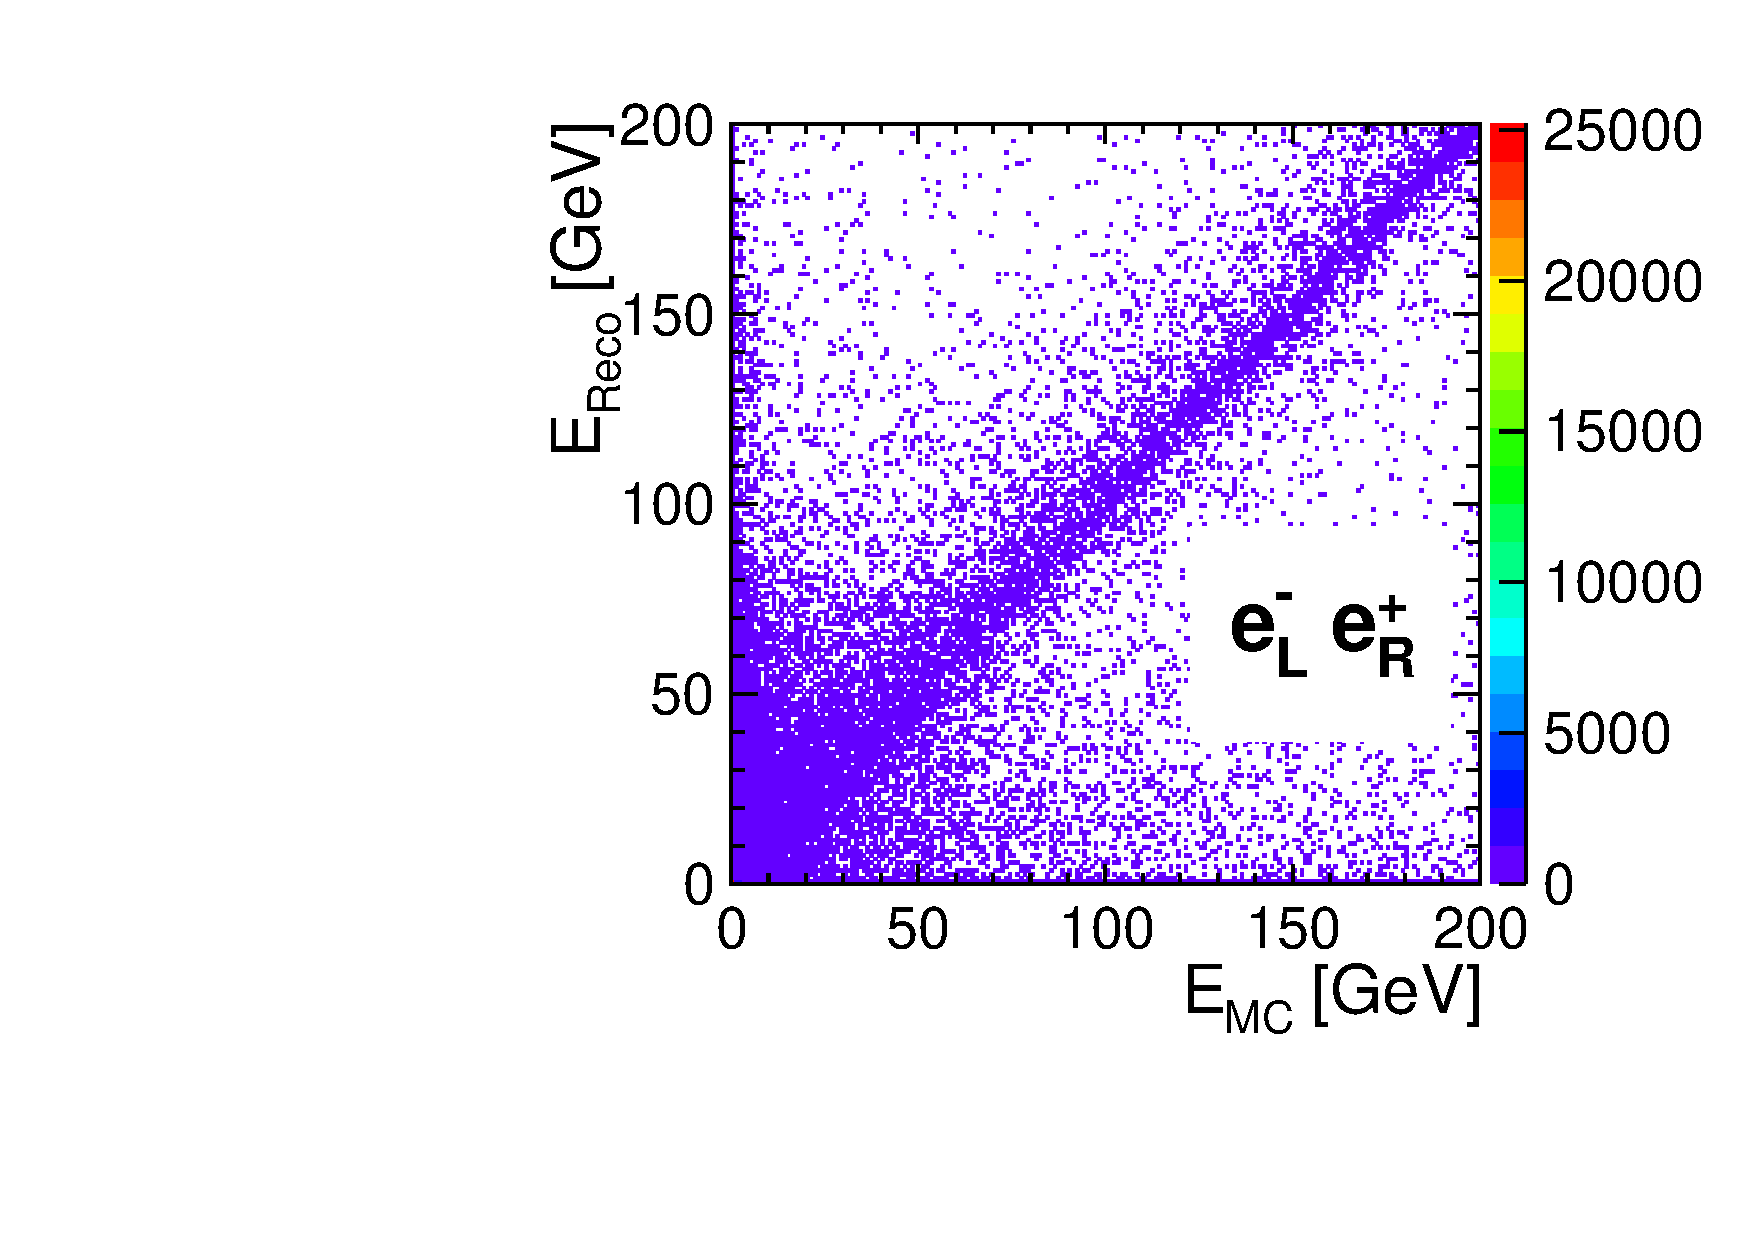
\includegraphics[width=\textwidth]{\imagepath/PhotonEnergy_2D_new_full.pdf}
    \end{minipage}

\end{frame}

% ----------------------------------------------------------------------------

\begin{frame}\frametitle{Back Up Slides \OrangeBF{1 lepton found in 1st cut}}

    \centering
    \includegraphics[width=0.7\textwidth]{\imagepath/Histflow3_isolep.pdf}

    \end{frame}

% ----------------------------------------------------------------------------

\end{document}
